\documentclass[oneside]{scrbook} %KOMA-Script book
% \documentclass[12pt,a4paper,twoside,openany]{book}
\usepackage[italian]{babel}
%Per i commenti
\usepackage{comment}
%Per l'interlinea
\usepackage{setspace}
%Codifica caratteri
\usepackage[utf8]{inputenc}
\usepackage{xspace}
\usepackage{eurosym}
%Fonts Scientifici
\usepackage{amsfonts}
\usepackage{amsmath}
\usepackage{amssymb}
\usepackage{textcomp}
%Pacchetto grafici
\usepackage{tikz}
\usepackage{pgfplots}
\pgfplotsset{/pgf/number format/use comma,compat=newest}
\usepackage{picture}
\usepackage{graphicx}
%Impostazioni tabelle avanzate e colorate
\usepackage{multicol}
\usepackage{multirow}
\usepackage{soul}
\usepackage{ulem}
\usepackage{booktabs}
%\usepackage{subfig}
\usepackage{subfigure}
\usepackage{array}
\usepackage{color}
\usepackage{colortbl}
%Pacchetto per gli pseudocodici
\usepackage{algpseudocode}
%\usepackage{listings}
\usepackage{listings,xcolor,courier,bookmark}
\usepackage{listingsutf8}
%Impostazioni tabelle avanzate
\usepackage{multicol}
\usepackage{multirow}
\usepackage{rotating}
%Impostazione per usare figure in minipage
\usepackage{float}
\definecolor{darkblue}{named}{blue}
\definecolor{darkred}{named}{red}
\definecolor{grau}{named}{gray}
%Per i margini
\usepackage{chngpage}
\sloppy
%Per usare captionof (fuori ambienti float)
\usepackage{caption}
\captionsetup{skip=4pt, minmargin=3cm, maxmargin=3cm}

\graphicspath{{Immagini/}}

\let\Righttorque\relax

\lstset{
	captionpos=b,
	commentstyle=\color[rgb]{0.133,0.545,0.133},
	keywordstyle=\color{darkblue},
	stringstyle=\color{purple},
	extendedchars=true,
	basicstyle=\small\ttfamily,
	showstringspaces=false,
	tabsize=2,
	numbers=left,
	numberstyle=\tiny,
	breakautoindent  = true,
	breakindent      = 2em,
	breaklines       = true,
	postbreak        = ,
	prebreak         = \raisebox{-.8ex}[0ex][0ex]{\Righttorque},
	showspaces=false,
	showtabs=false,
	showstringspaces=false,
	language=C++,
	frame=single,
	morecomment=[s]{°°},
	inputpath=Sorgenti/
}

\renewcommand*{\lstlistingname}{Codice}
\renewcommand*{\lstlistlistingname}{Elenco dei codici}

\usepackage{fancyhdr}
\pagestyle{fancy}
\renewcommand{\chaptermark}[1]{\markboth{\MakeUppercase{\thechapter.\ #1}}{}}
\fancypagestyle{plain} %stile delle pagine anche a quella iniziale del capitolo

\fancyhead{}
\fancyfoot{}

\fancyhead[R]{\bfseries \nouppercase{\leftmark}}
\fancyhead[L]{
	\includegraphics*[scale=0.8]{logo_dieti2.png}
}
\fancyfoot[R]{\thepage}
\fancyfoot[L]{Tesina di Impianti di Elaborazione}
\renewcommand{\headrulewidth}{0.4pt}
\renewcommand{\footrulewidth}{0.4pt}

\date{}
\cfoot{}
\usepackage{eso-pic,graphicx}

%Per sottosezioni
\setcounter{secnumdepth}{4}
\setcounter{tocdepth}{4}

\begin{document}

	% Per evitare che i collegamenti nell'indice abbiano i riquadri rossi
	\hypersetup {linkbordercolor=white}

	\AddToShipoutPicture{\AtPageCenter{\makebox(0,0){
\includegraphics{logo.png}}}}
	\frontmatter
	\pagenumbering{Roman}

	\begin{titlepage}
		\centering
		%{\Huge \textsc{Università degli Studi di Napoli ``Federico II''}}

		%\vspace*{\stretch{2.5}}

		%
\includegraphics[width=1\linewidth]{logo_federico_II.png}

		
\includegraphics[width=1\linewidth]{logo_dieti2.png}

		\vspace*{2cm}

		{\Huge \textsl{Tesina di\\IMPIANTI DI ELABORAZIONE}\par}

		\vspace*{2cm}

		{\huge \text{Prof. Domenico Cotroneo}}

		\vspace*{5cm}

		{\LARGE \textit{Andrea Scognamiglio - Matr. M63/598\\Cristian Tommasino - Matr. M63/615}}

		\vspace*{2.5cm}

		{\Large \textsc{A.A. 2017/2018}}
	\end{titlepage}

	\setcounter{page}{1}

	\newpage
	\tableofcontents

	\newpage
	\mainmatter

	% !TEX root = ./main.tex
% !TEX encoding = UTF-8 Unicode
% !TEX program = pdflatex
% !TeX spellcheck = it_IT

\graphicspath{{Immagini/},{Immagini/prodotto_matrici/}}

\chapter{Prodotto Matrici}

\section{Traccia}
Confrontare in Java e in C++ l'esecuzione del prodotto di matrici quadrate
di dimensione: 10000, 100000, 1000000.\\
Tale benchmark è utilizzato per valutare le prestazione dei
due linguaggi di programmazione.\\

\section{System Under Test}
La macchina target utilizzata per l'esecuzione degli algoritmi è:
\begin{itemize}
  \item \textbf{Processore}: Intel(R) Core(TM) i7-7700HQ @ 2.80GHz
  \item \textbf{Memoria Ram}: 16GB DDR4-2400MHz
  \item \textbf{Tipo sistema}: Windows 10 64bit, processore basato su x64
  \item \textbf{Storage}: SSD Kingston M.2.SATA 480GB
\end{itemize}

\section{Soluzione}
Il classico algoritmo di prodotto matriciale(\textbf{IKJ Algorithm}), ha una complessità computazionale
$O(n^3)$, dunque, per le dimensioni assegnate, richiederebbe un tempo di esecuzione
elevato.\\
Per questo motivo si è scelto di ridurre notevolmente le dimensioni delle matrici
ed utilizzare l'algoritmo di \textbf{Strassen}, avente complessità computazionale $O(n^{2,81})$.\\

\subsection{Strassen Algorithm}
L'algoritmo di Strassen calcola il prodotto di matrici quadrate assumendo che siano
del tipo $2^n \times 2^n$. \\ In particolare: $C=A \cdot B$ con $A,B,C \in R^{2^n \times 2^n}$.\\
Dividendo le matrici A,B e C in blocchi si ottiene:
\\
\[
A =
\begin{bmatrix}
  A_{1,1} & A_{1,2} \\
  A_{2,1} & A_{2,2}
\end{bmatrix}
B =
\begin{bmatrix}
  B_{1,1} & B_{1,2} \\
  B_{2,1} & B_{2,2}
\end{bmatrix}
C =
\begin{bmatrix}
  C_{1,1} & C_{1,2} \\
  C_{2,1} & C_{2,2}
\end{bmatrix}
\]\\
con $A, B, C \in R^{2^{n-1} \times 2^{n-1}}$.\\
\\
La matrice risultato si ottiene come:\\
$$C_{1,1} = A_{1,1}B_{1,1}+A_{1,2}B_{2,1}$$
$$C_{1,2} = A_{1,1}B_{1,2}+A_{1,2}B_{2,2}$$
$$C_{2,1} = A_{2,1}B_{1,1}+A_{2,2}B_{2,1}$$
$$C_{2,2} = A_{2,1}B_{1,2}+A_{2,2}B_{2,2}$$
\\
Utilizzando tale tecnica, il numero di prodotti matriciali da svolgere è 8.\\
Al fine di ridurre il numero di moltiplicazioni necessarie a generare le matrici
$C_{x,y}$, è possibile definire le seguenti
matrici:\\
$$M_1 = (A_{1,1}+A_{2,2})(B_{1,1}+B_{2,2})$$
$$M_2 = (A_{2,1}+A_{2,12})B_{1,1}$$
$$M_3 = A_{1,1}(B_{1,2}-B_{2,2})$$
$$M_4 = A_{2,2}(B_{2,1}-B_{1,1})$$
$$M_5 = (A_{1,1}+A_{1,2})B_{2,2}$$
$$M_6 = (A_{2,1}-A_{1,1})(B_{1,1}+B_{1,2})$$
$$M_7 = (A_{1,2}-A_{2,2})(B_{2,1}+B_{2,2})$$
Quindi la matrice risultato si ottime come:
$$C_{1,1} = M_1 + M_4 - M_5 + M_7$$
$$C_{1,2} = M_3 + M_5$$
$$C_{2,1} = M_2 + M_4$$
$$C_{2,2} = M_1 - M_2 + M_3 + M_6$$

\clearpage
\section{Analisi}

Gli algoritmi sono stati testati su matrici quadrate di dimensione 1024, 2048 e 4096.\\
Come analisi preliminare sono state effettuate 5 osservazioni indipendenti, al variare di N.\\
Per rendere le esecuzioni indipendenti, gli algoritmi sono stati eseguiti tramite uno
script batch.\\
L'algoritmo in Java è stato testato anche disattivando il \textbf{JIT}(Just In Time)
compiler, il quale ottimizza l'esecuzione dell'algoritmo, e in C++ abilitando anche
l'ottimizzazione \textbf{O2} (per codice più veloce e snello).\\

\subsection{Numero di esperimenti}

Per determinare la dimensioni dei campioni si è fatto utilizzo della seguente formula:
$$N= {\biggl({{\frac{100*z*s}{r*\overline{x}}}\biggr)}^2}$$
Dove:
\begin{itemize}
  \item \textbf{\textit{z}}: $(1-{\alpha / 2})$-quantile della distribuzione normale
  per ottenere un intervallo di confidenza $100\cdot(1-\alpha)$;
  \item \textbf{\textit{s}}: deviazione standard del campione;
  \item \textbf{\textit{r}}: accuratezza percentuale;
  \item \textbf{{$\overline{\textit{x}}$}}: media del campione.
\end{itemize}

Nel caso in analisi, l'intervallo di confidenza desiderato è del 95\%, quindi
$\alpha = 0.05$ ed $ r = 5 $.

Nelle seguenti figure sono riportati i tempi raccolti e le relative statistiche
utilizzate per la valutazione del parametro \textbf{N}.
\begin{figure}[!htbp]
  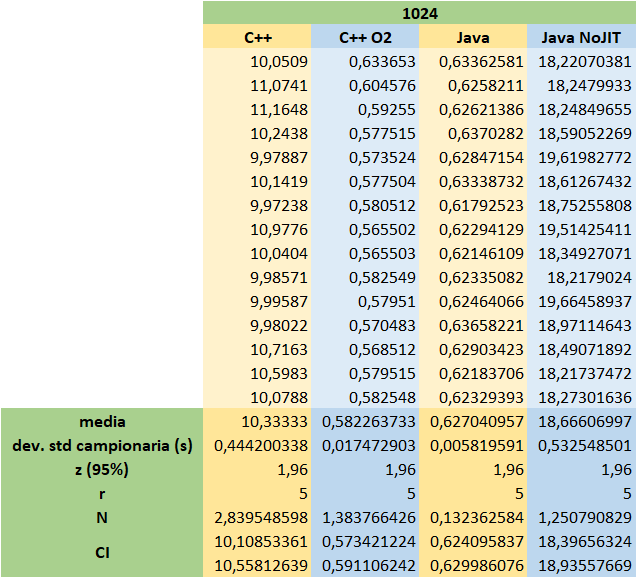
\includegraphics[width=1\linewidth,keepaspectratio]{tempi_1024}
  \caption{Esperimenti matrici 1024x1024}
  \label{prodottomatrici_tempi_1024}
\end{figure}

\begin{figure}[!htbp]
  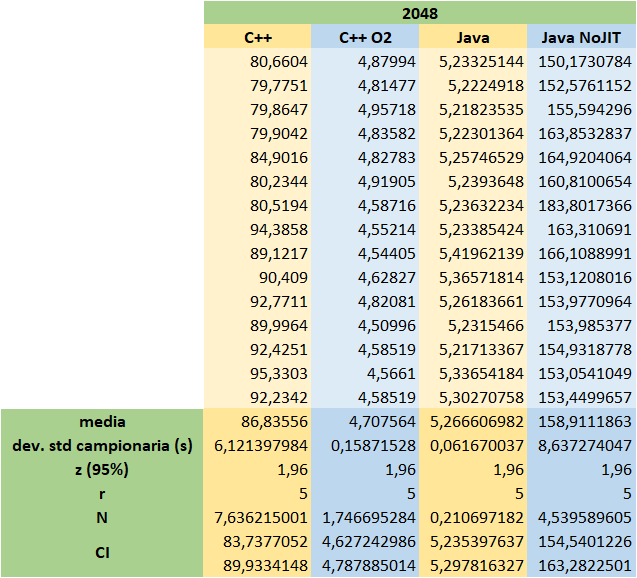
\includegraphics[width=1\linewidth,keepaspectratio]{tempi_2048}
  \caption{Esperimenti matrici 2048x2048}
  \label{prodottomatrici_tempi_2048}
\end{figure}

\begin{figure}[!htbp]
  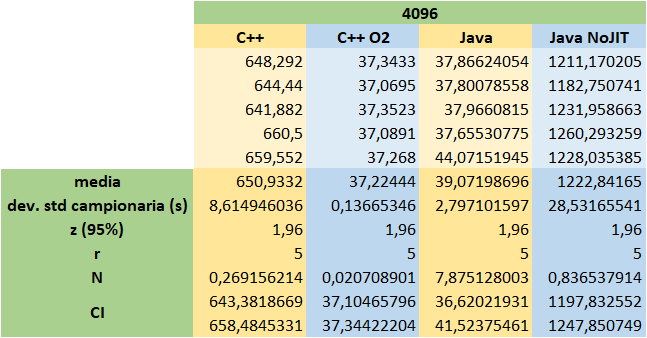
\includegraphics[width=1\linewidth,keepaspectratio]{tempi_4096}
  \caption{Esperimenti matrici 4096x4096}
  \label{prodottomatrici_tempi_4096}
\end{figure}

\clearpage

A valle dei 5 esperimenti svolti al variare della dimensione delle matrici,
considerando il caso peggiore, il numero di esperimenti necessario,
risulta essere 8.\\

\subsection{Esperimenti}

Nelle figure seguenti sono riportati i tempi di esecuzione degli 8 esperimenti
sull'algoritmo di Strassen, svolto nei differenti linguaggi.\\

\begin{figure}[!htbp]
  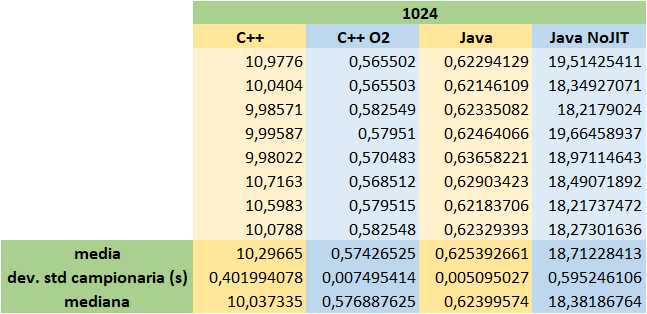
\includegraphics[width=1\linewidth,keepaspectratio]{tempi_8_1024}
  \caption{Esperimenti matrici 1024x1024}
  \label{prodottomatrici_tempi_8_1024}
\end{figure}

\begin{figure}[!htbp]
  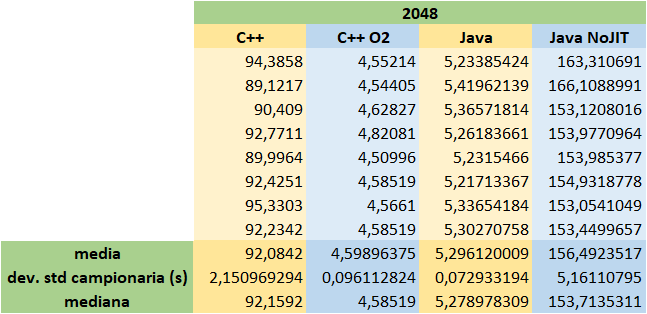
\includegraphics[width=1\linewidth,keepaspectratio]{tempi_8_2048}
  \caption{Esperimenti matrici 2048x2048}
  \label{prodottomatrici_tempi_8_2048}
\end{figure}

\begin{figure}[!htbp]
  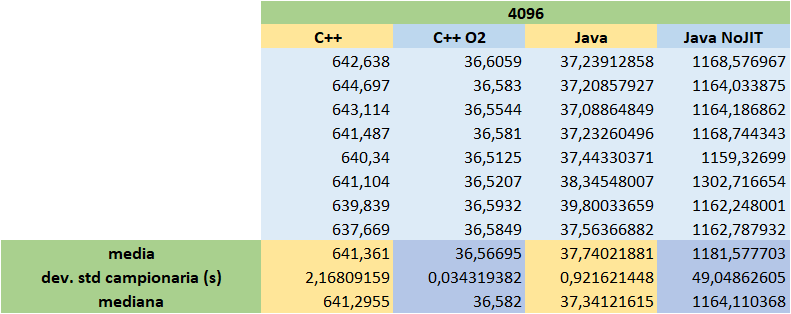
\includegraphics[width=1\linewidth,keepaspectratio]{tempi_8_4096}
  \caption{Esperimenti matrici 4096x4096}
  \label{prodottomatrici_tempi_8_4096}
\end{figure}

\clearpage

In seguito sono riportati i grafici del confronto dei tempi di Java e C++, sia
nelle loro versioni ottimizzate dal compilatore sia in quelle non ottimizzate.\\

\begin{figure}[!htbp]
  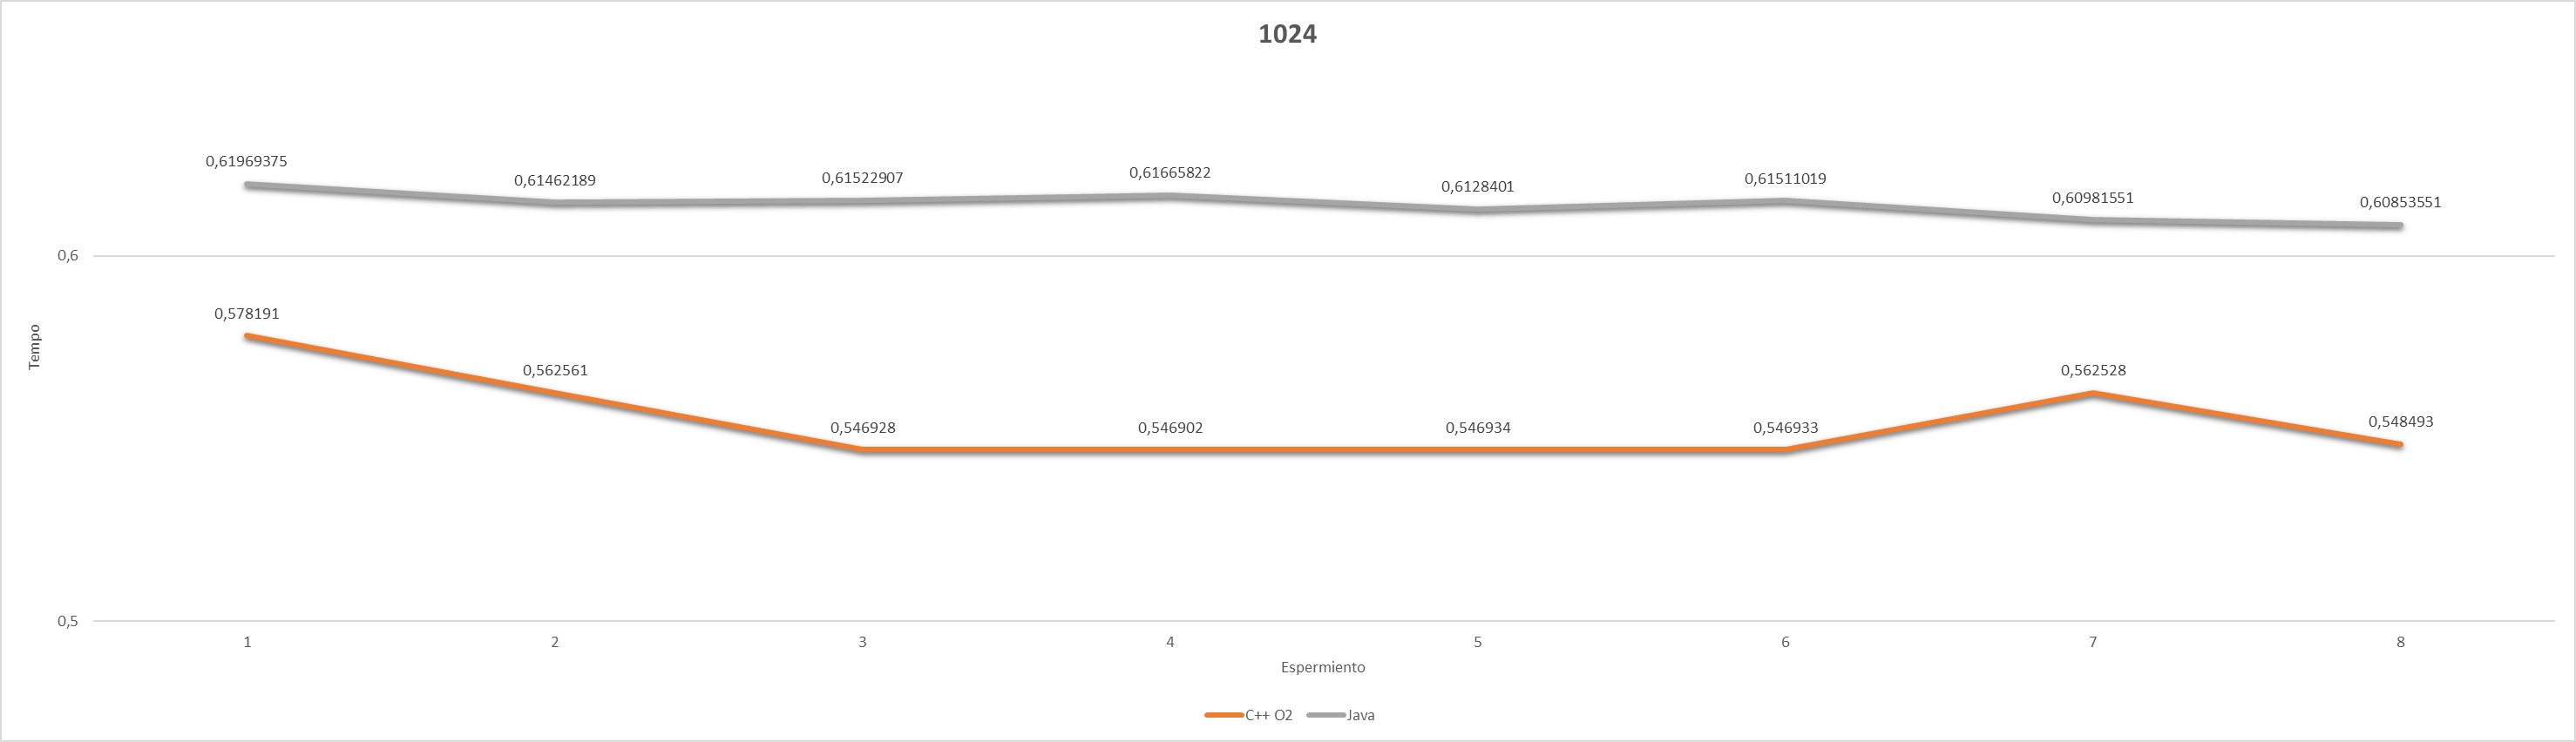
\includegraphics[width=1\linewidth,keepaspectratio]{grafico_tempi_1024_2}
  \caption{Confronto tempi \textbf{Java} vs \textbf{C++ O2} 1024x1024}
  \label{prodottomatrici_grafico_tempi_1024_2}
\end{figure}

\begin{figure}[!htbp]
  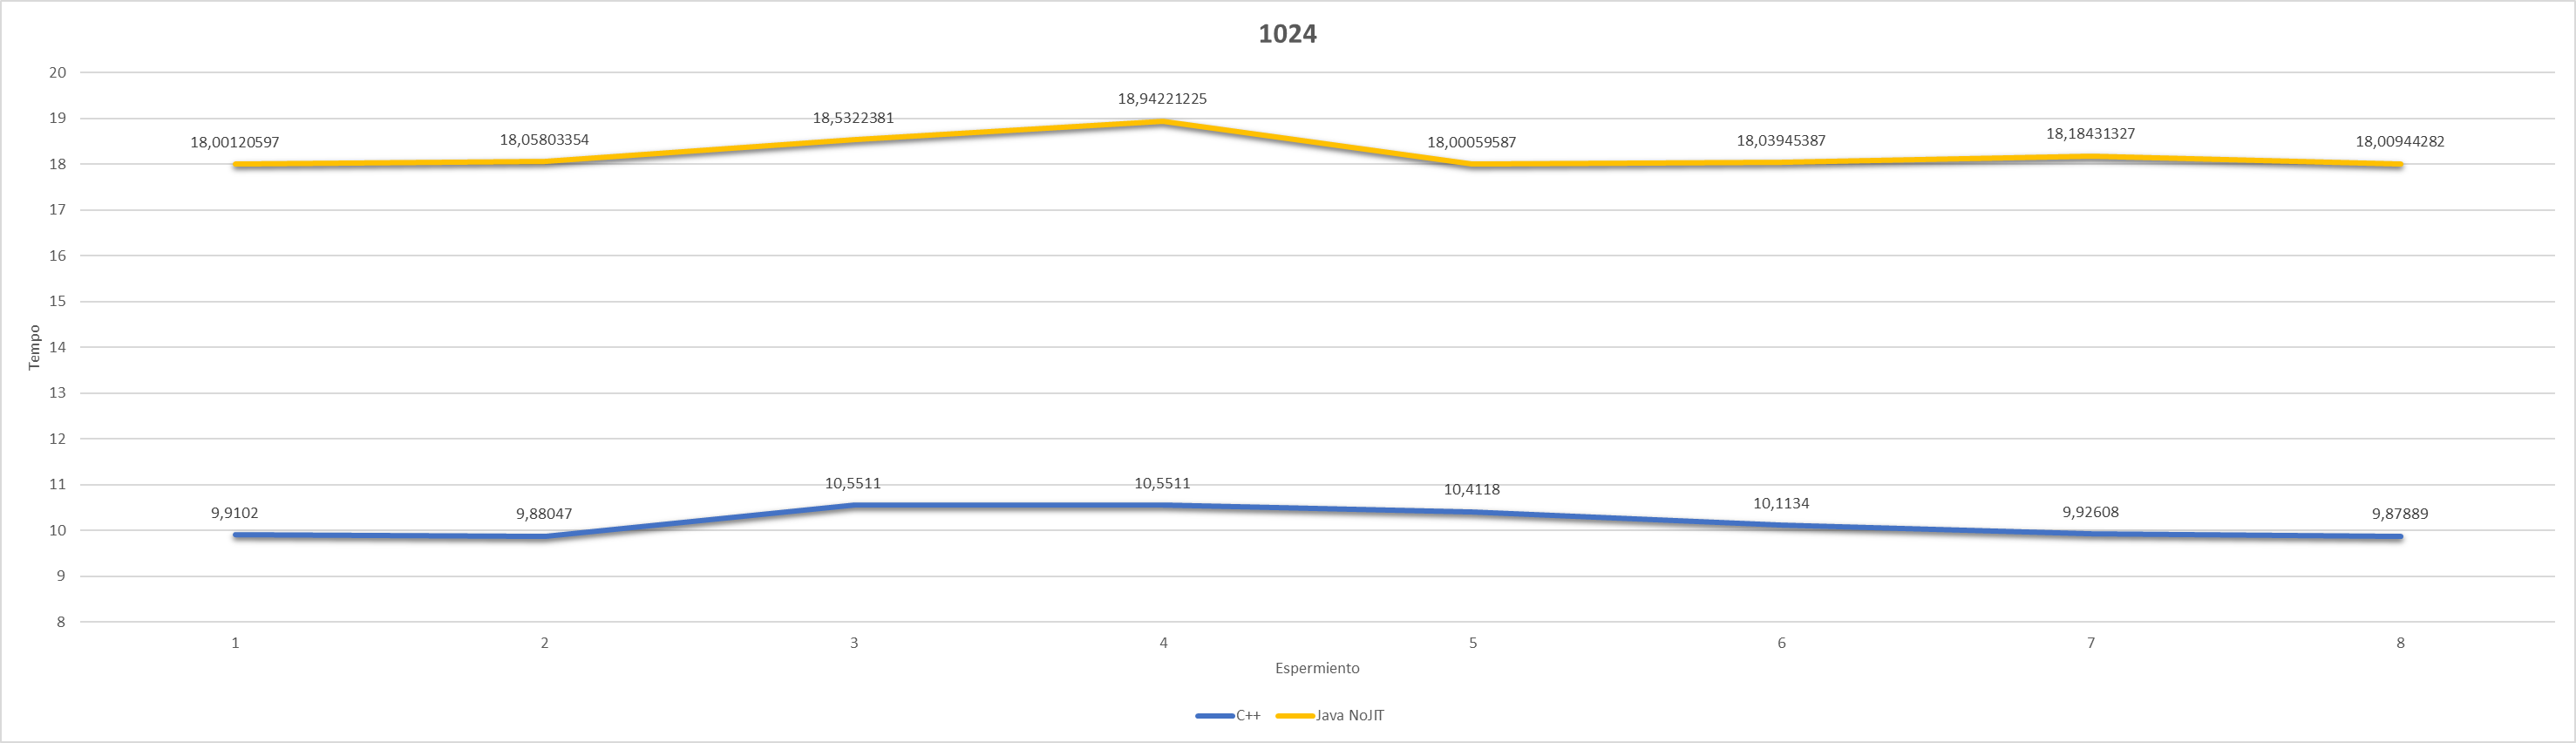
\includegraphics[width=1\linewidth,keepaspectratio]{grafico_tempi_1024_1}
  \caption{Confronto tempi \textbf{Java NoJIT} vs \textbf{C++} 1024x1024}
  \label{prodottomatrici_grafico_tempi_1024_1}
\end{figure}

\clearpage

\begin{figure}[!htbp]
  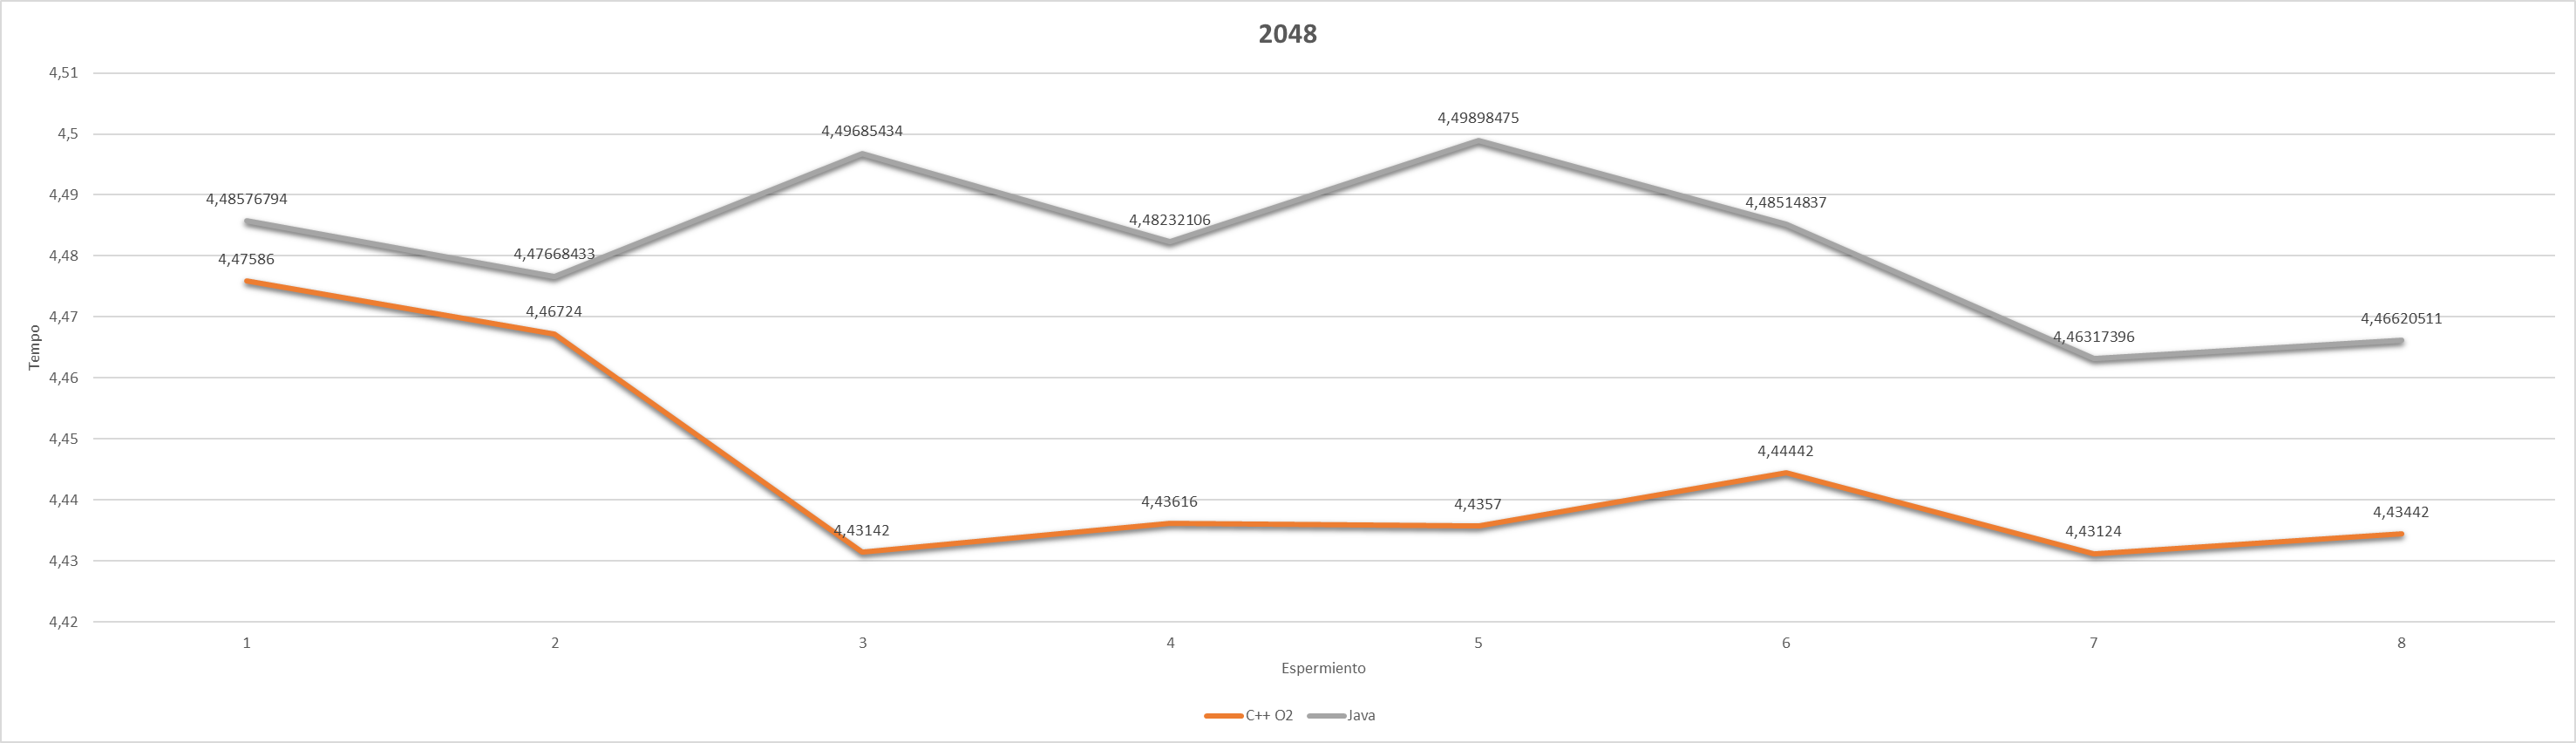
\includegraphics[width=1\linewidth,keepaspectratio]{grafico_tempi_2048_2}
  \caption{Confronto tempi \textbf{Java} vs \textbf{C++ O2} 2048x2048}
  \label{prodottomatrici_grafico_tempi_2048_2}
\end{figure}

\begin{figure}[!htbp]
  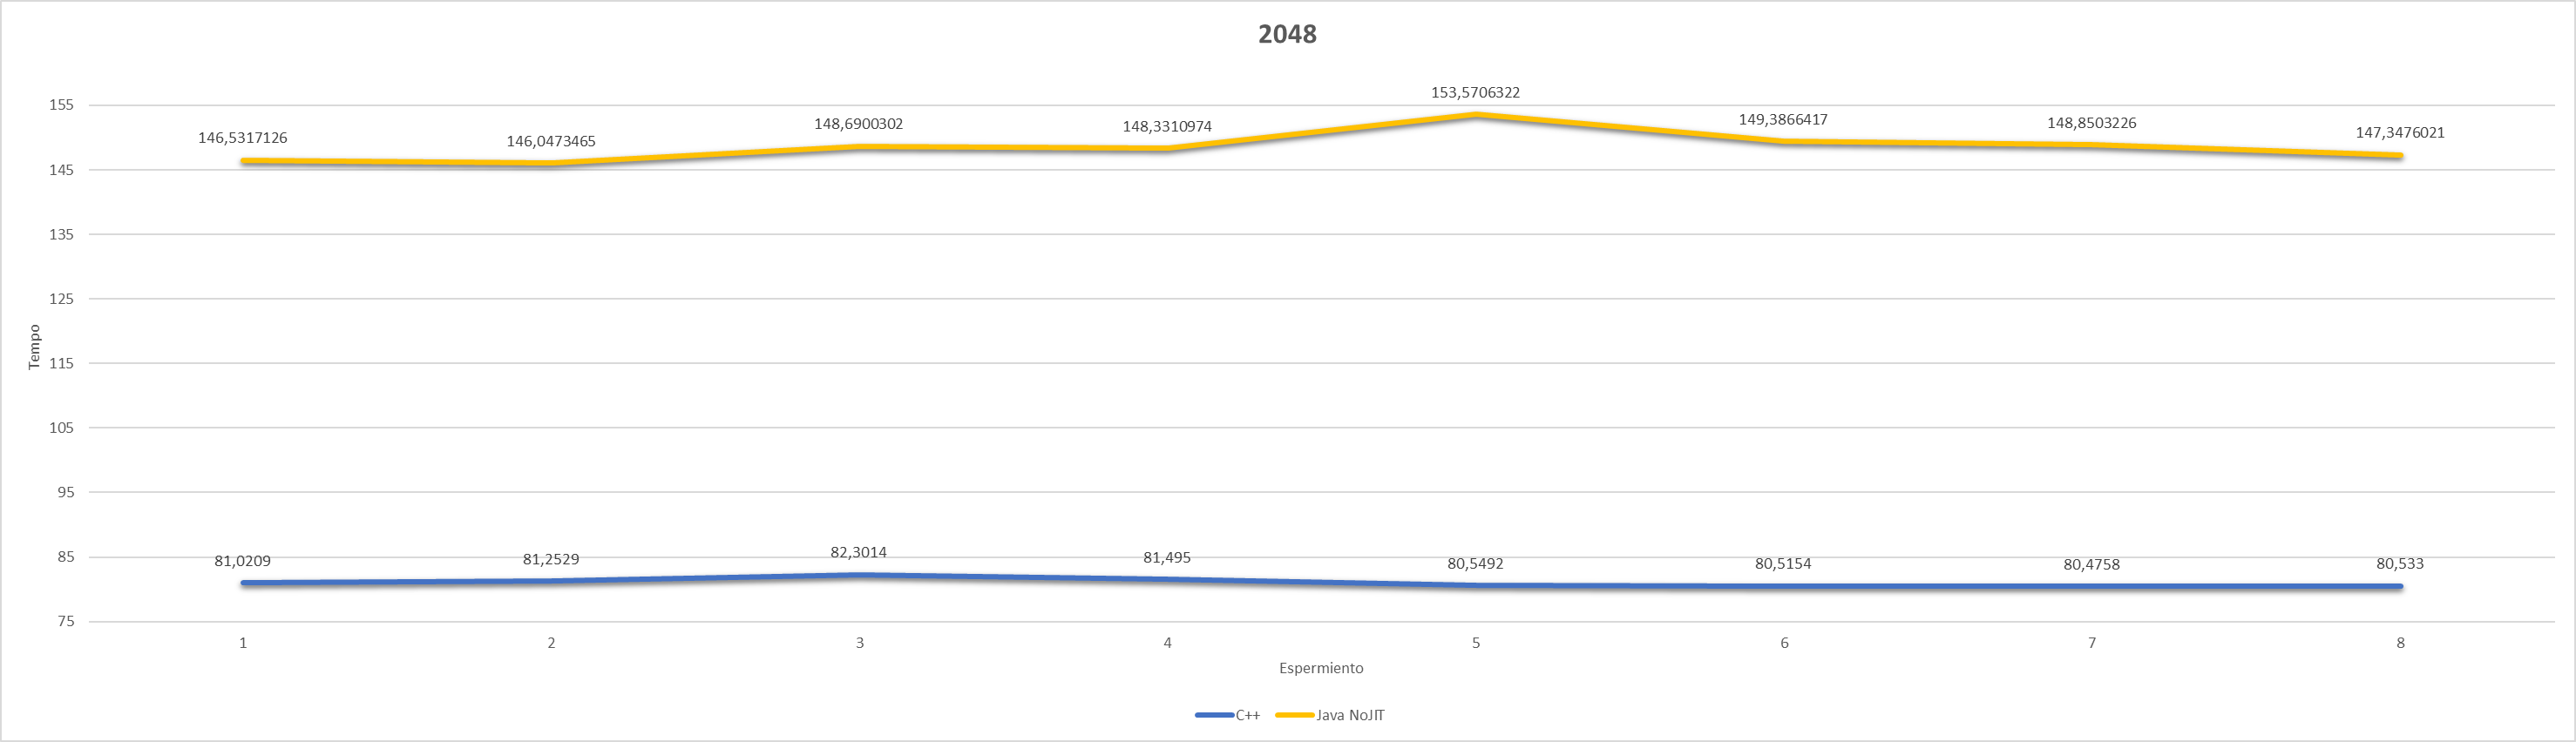
\includegraphics[width=1\linewidth,keepaspectratio]{grafico_tempi_2048_1}
  \caption{Confronto tempi \textbf{Java NoJIT} vs \textbf{C++} 2048x2048}
  \label{prodottomatrici_grafico_tempi_2048_1}
\end{figure}

\clearpage

\begin{figure}[!htbp]
  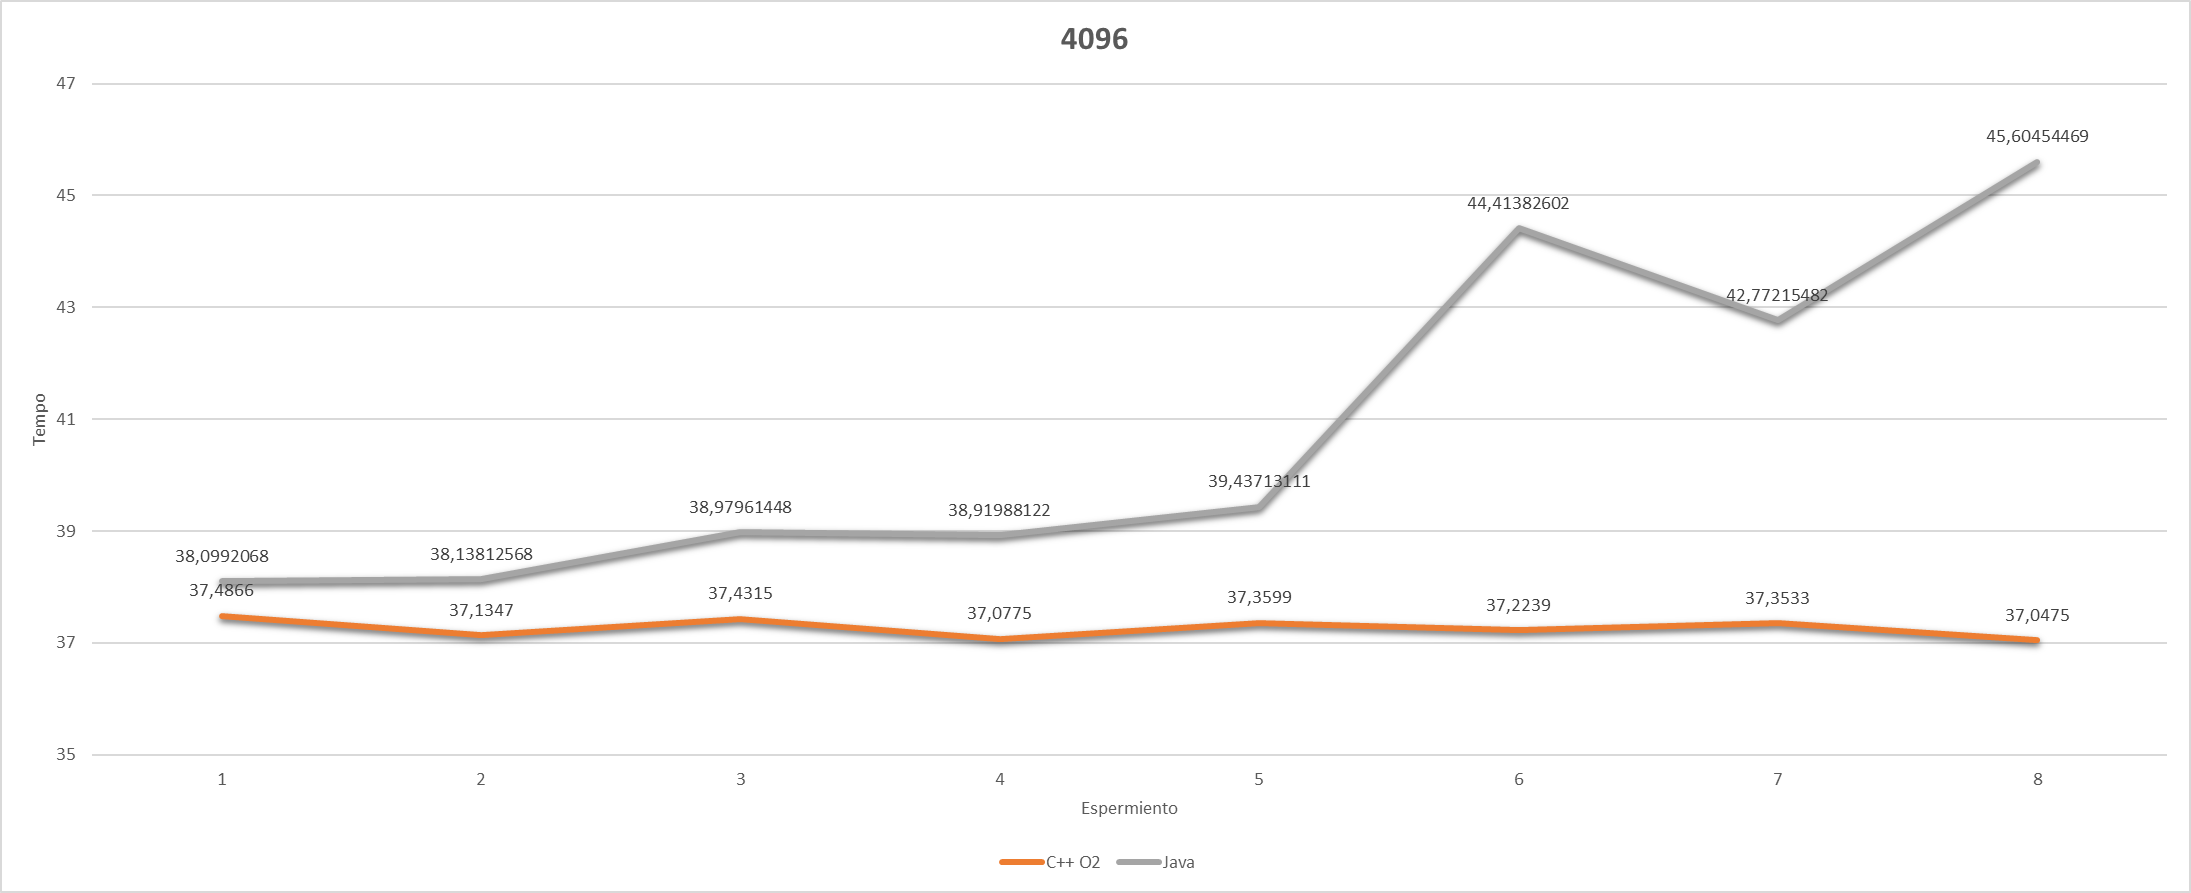
\includegraphics[width=1\linewidth,keepaspectratio]{grafico_tempi_4096_2}
  \caption{Confronto tempi \textbf{Java} vs \textbf{C++ O2} 4096x4096}
  \label{prodottomatrici_grafico_tempi_4096_2}
\end{figure}

\begin{figure}[!htbp]
  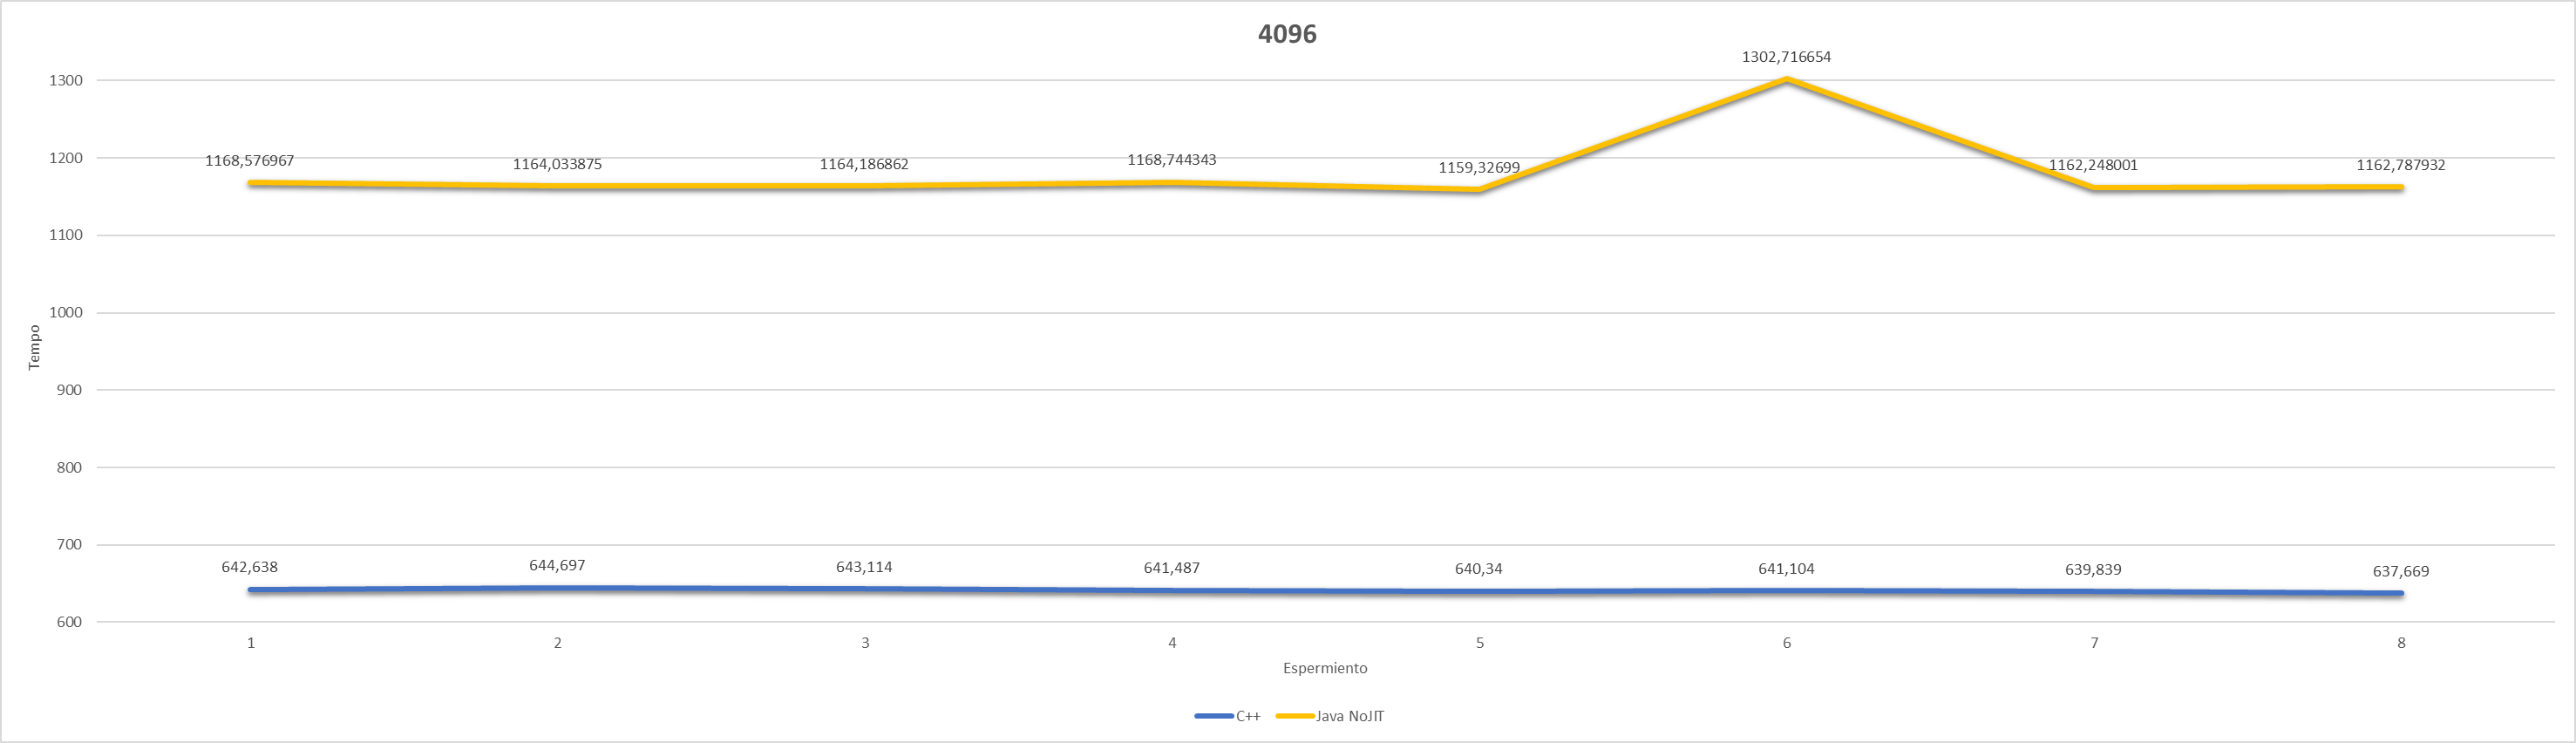
\includegraphics[width=1\linewidth,keepaspectratio]{grafico_tempi_4096_1}
  \caption{Confronto tempi \textbf{Java NoJIT} vs \textbf{C++} 4096x4096}
  \label{prodottomatrici_grafico_tempi_4096_1}
\end{figure}

Si noti che, per tutte le dimensioni considerate, Java con JIT e C++ O2 sono
molto più performanti delle corrispondenti versioni non ottimizzate.\\
\clearpage
\subsection{Significatività dei risultati}

Per verificare la significatività statistica delle 8 osservazioni fatte è fondamentale
dimostrare che le distribuzioni non siano statisticamente equivalenti, ovvero che
appartengano a popolazioni differenti.\\
A tal fine, la statistica inferenziale mette a disposizione diversi test(parametrici e non),
i quali possono essere applicati in modo opportuno solo conoscendo la natura
della distribuzione analizzata.\\
In particolare, è di interesse definire la normalità o meno dei dati che si hanno
a disposizione.\\
Per studiare la normalità della distribuzione si possono utilizzare i seguenti
parametri:

\begin{itemize}
  \item \textbf{Indice di Asimmetria}: cerca di fornire una misura sulla mancanza
  di simmetria in una distribuzione, il valore 0 è una condizione necessaria, ma
  non sufficiente, per la simmetria;
  \item \textbf{Curtosi}: fornisce una misura sull'appiattimento della curva,
  il valore dell'indice corrispondente ad una distribuzione normale è 0;
  \item \textbf{Coefficiente di Variazione}: permette di determinare la dispersione
  dei valori intorno alla media indipendentemente dall'unità di misura.
\end{itemize}

\'E possibile utilizzare, come test di verifica della normalità di una distribuzione,
il test di \textbf{Shapiro-Wilk} o test della bontà di adattamento.\\
Tale test restituisce il valore W, compreso nell’intervallo [0, 1], che per
valori vicini allo 0 indica una distribuzione \textbf{skewed}, mentre per valori
vicini ad 1 indica una distribuzione normale.\\
Un'ulteriore tecnica per la verifica della normalità dei dati prevede di
osservare il plot \textbf{Quantile-Quantile}, che presenta sull'asse delle ascisse
i valori tipici dei quantili di una normale, mentre sull'asse delle ordinate i
valori dei quantili della distribuzione osservata.\\
Questa tecnica visiva è molto robusta all'errore, e per questo motivo, molto usata.\\
L'interpretazione del plot Q-Q è abbastanza semplice: se i punti risultanti sono
difficilmente approssimabili con una retta, allora si può affermare, con buon
margine statistico, che è rifiutata l'ipotesi nulla che quella osservata sia una
distribuzione normale.\\
Viceversa, è possibile continuare a studiare con ulteriori parametri e test, la
normalità della distribuzione.\\

\clearpage

\subsubsection{Distribuzioni C++ O2}
Nella seguente figura sono riportate le distribuzioni, al crescere di N, del
linguaggio C++ con ottimizzazione O2 attiva.

\begin{figure}[!htbp]
  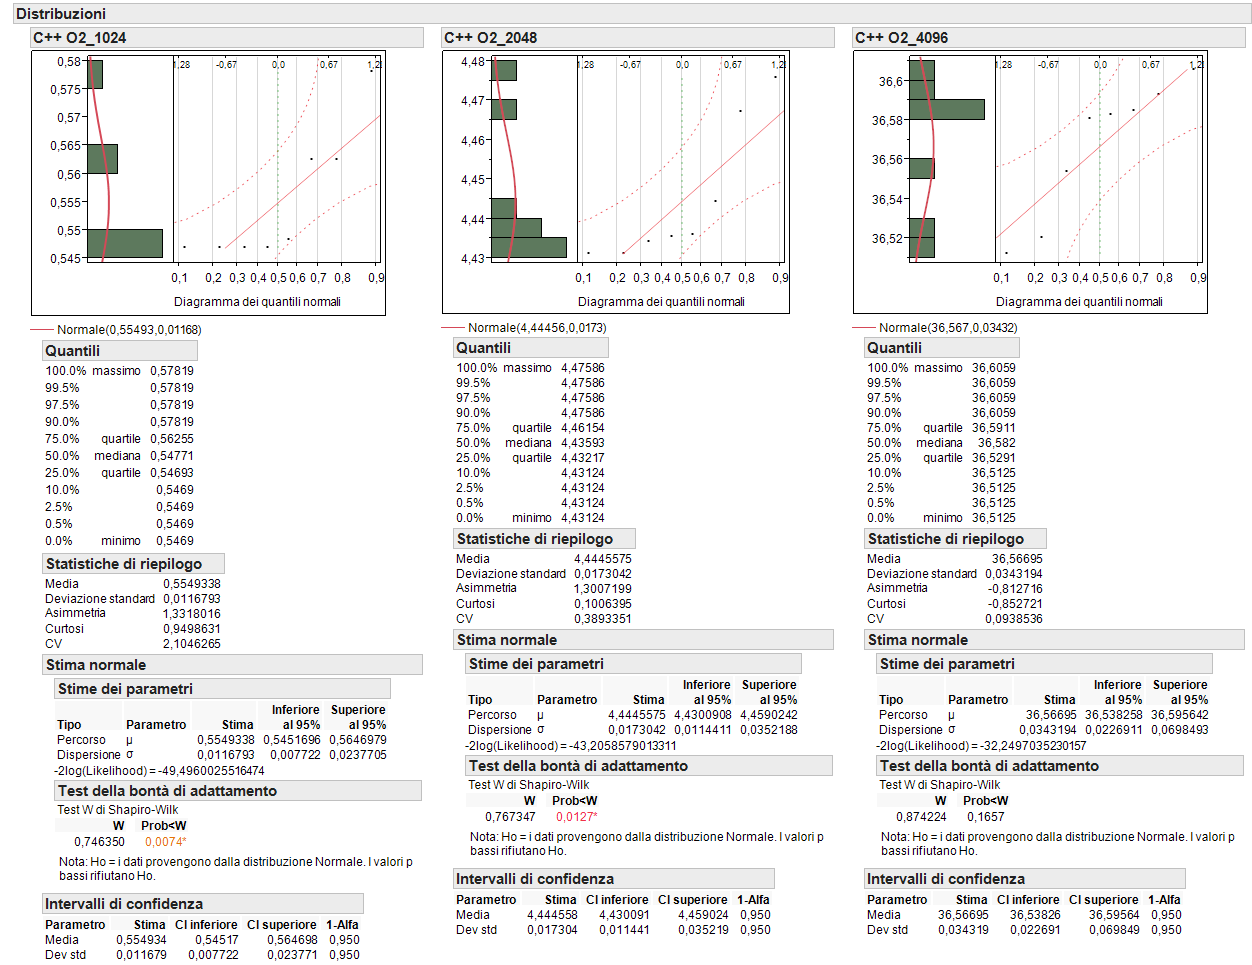
\includegraphics[width=1\linewidth,keepaspectratio]{distribuzione_cppO2}
  \caption{Distribuzioni osservazioni in C++ O2}
  \label{prodottomatrici_distribuzione_cppO2}
\end{figure}
Dalla \figurename~\ref{prodottomatrici_distribuzione_cppO2} si nota
che la distribuzione per dimensione 2048 non è normale poiché è rifiutata
l'ipotesi nulla del test Shapiro-Wilk, a differenza delle distribuzioni a 1024 e 4096,
in cui l'ipotesi nulla non è rigettata e quindi non è possibile affermare che
quella osservata non sia una normale.\\
Osservando il plot Q-Q si osserva che la distribuzione a 1024 non è approssimabile con una
retta e considerando anche gli indici di asimmetria e curtosi è possibile affermare che
la distribuzione è non normale, mentre per la distribuzione a 4096, anche se dal plot
Q-Q si potrebbe dire normale, osservando l'indice di curtosi è possibile rifiutare
la normalità.
\clearpage
\subsubsection{Distribuzioni C++ }
Nella seguente figura sono riportate le distribuzioni, al crescere di N, del
linguaggio C++.

\begin{figure}[!htbp]
  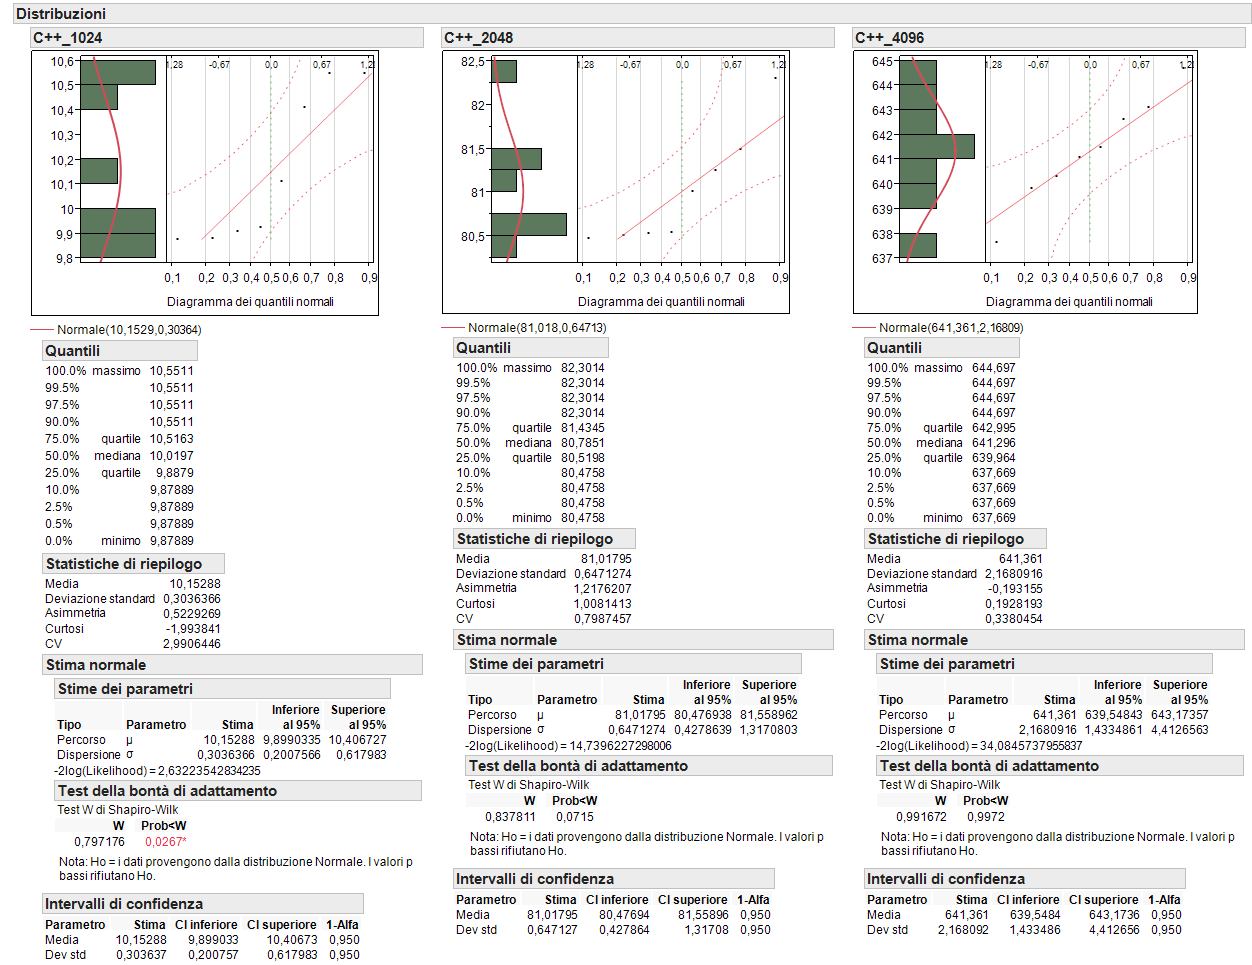
\includegraphics[width=1\linewidth,keepaspectratio]{distribuzione_cpp}
  \caption{Distribuzioni osservazioni in C++}
  \label{prodottomatrici_distribuzione_cpp}
\end{figure}

Dalla \figurename~\ref{prodottomatrici_distribuzione_cpp} si nota
che le distribuzioni per dimensioni 1024 e 4096 non sono normali poiché è rifiutata
l'ipotesi nulla del test Shapiro-Wilk, a differenza della distribuzione 2048,
in cui l'ipotesi nulla non è rigettata e quindi non è possibile affermare
che quella osservata non sia una normale.\\
Osservando il plot Q-Q si osserva che la distribuzione con N pari a 2048 è approssimabile con una
retta e considerando anche gli indici di asimmetria e curtosi è possibile osservare che
la distribuzione sia normale.\\
\clearpage
\subsubsection{Distribuzioni Java}
Nella seguente figura sono riportate le distribuzioni, al crescere di N, del
linguaggio Java.

\begin{figure}[!htbp]
  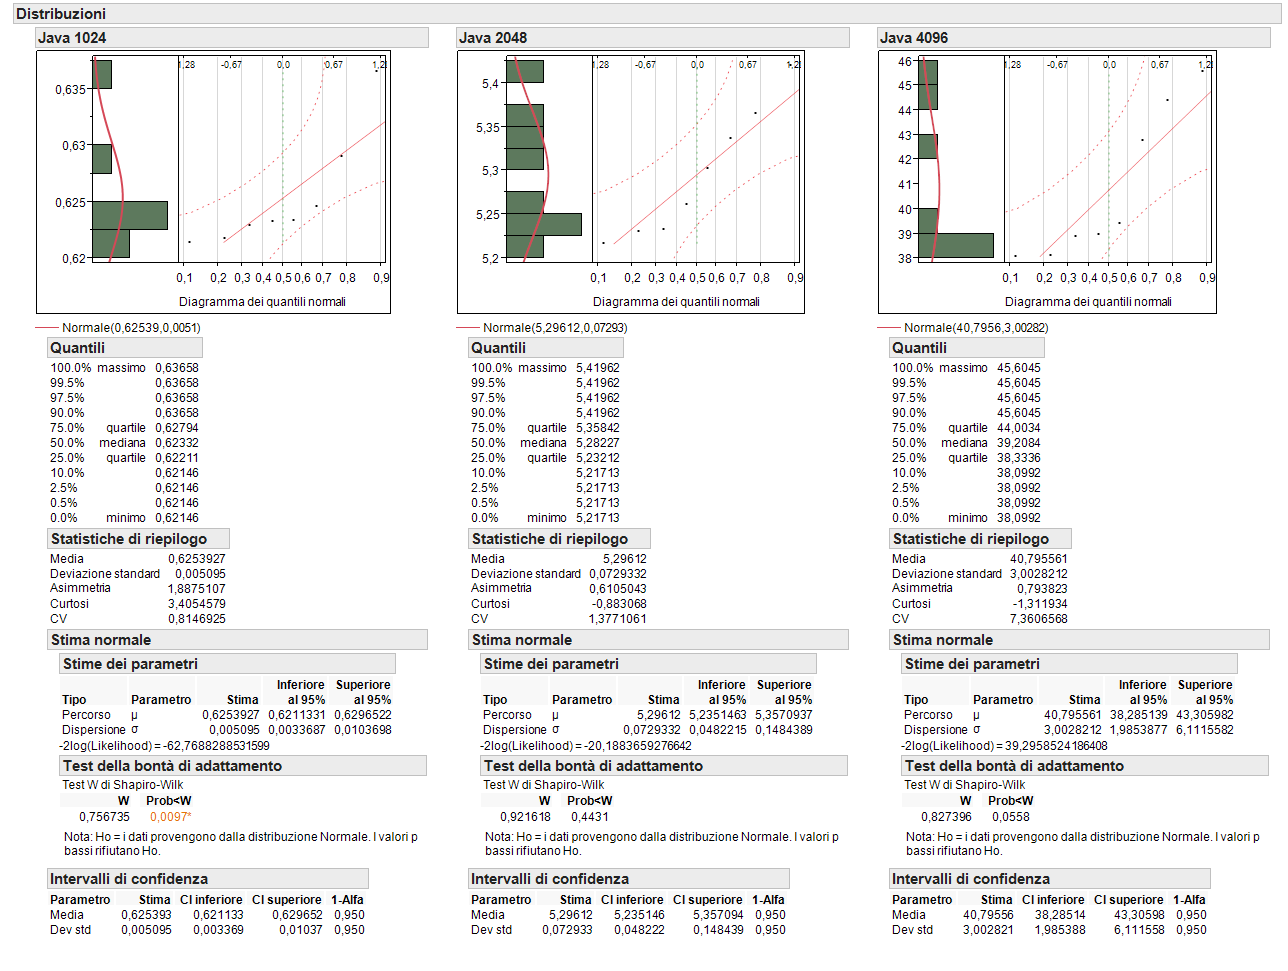
\includegraphics[width=1\linewidth,keepaspectratio]{distribuzione_java}
  \caption{Distribuzioni osservazioni in Java}
  \label{prodottomatrici_distribuzione_java}
\end{figure}

Dalla \figurename~\ref{prodottomatrici_distribuzione_java} si nota
che la distribuzione per dimensione 1024 non è normale, essendo rifiutata
l'ipotesi nulla del test Shapiro-Wilk, a differenza delle distribuzioni 2048 e
4096, in cui l'ipotesi nulla non è rigettata e quindi non è possibile affermare
che quella osservata non sia una normale.\\
Osservando il plot Q-Q si osserva che la distribuzione con N pari a 2048
è approssimabile con una retta, e considerando anche l'indice di asimmetria
e di curtosi è possibile osservare che la distribuzione sia normale, mentre
per la distribuzione con N pari a 4096 è possibile rigettare l'ipotesi di normalità.\\

\clearpage
\subsubsection{Distribuzioni Java No JIT}
Nella seguente figura sono riportate le distribuzioni, al crescere di N, del
linguaggio Java con JIT Compiler disattivato.

\begin{figure}[!htbp]
  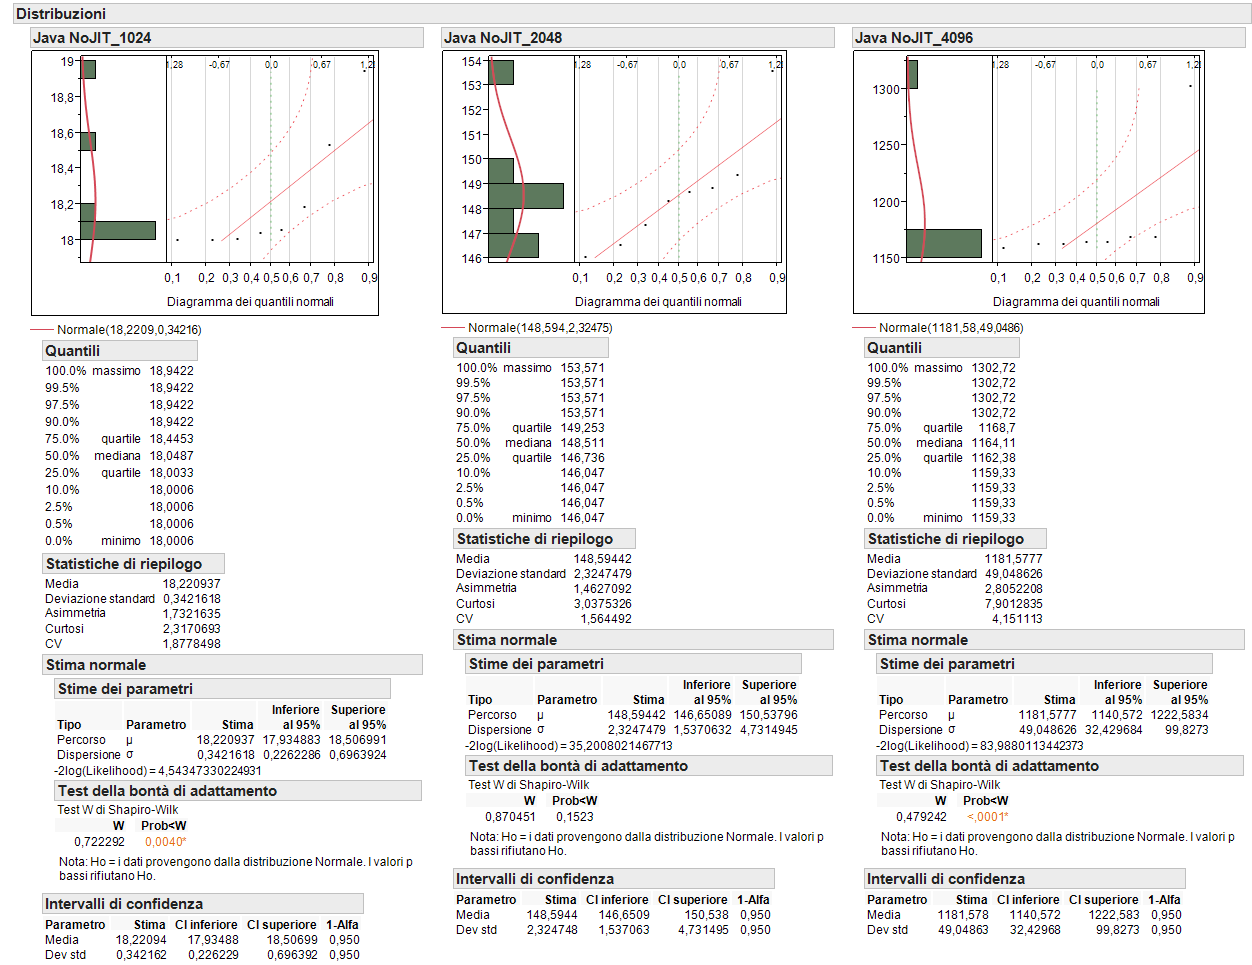
\includegraphics[width=1\linewidth,keepaspectratio]{distribuzione_javaNoJIT}
  \caption{Distribuzioni osservazioni in Java NoJIT}
  \label{prodottomatrici_distribuzione_javaNoJIT}
\end{figure}

Dalla \figurename~\ref{prodottomatrici_distribuzione_javaNoJIT} si nota
che le distribuzioni per dimensione pari a 1024 e 2048 non sono normali, essendo
rifiutata l'ipotesi nulla del test Shapiro-Wilk, a differenza della distribuzione
4096, in cui l'ipotesi nulla non è rigettata e quindi non è possibile affermare
che quella osservata non sia una normale.\\
Osservando il plot Q-Q si osserva che la distribuzione con N pari a 4096 è
approssimabile con una retta e considerando gli indici di asimmetria e di
curtosi è possibile affermare che la distribuzione è normale.\\

\clearpage
\subsubsection{Intervallo di confidenza}
Un’ultima osservazione da dover fare riguarda gli intervalli di confidenza ottenuti in
analisi preliminare.\\
A causa della non normalità della maggioranza delle distribuzioni, si è deciso di
utilizzare la mediana come indice di tendenza centrale. \\
Confrontando le mediane delle distribuzioni dei campioni
con gli intervalli di confidenza ottenuti in analisi preliminare si nota che non
tutte le distribuzioni rispettano le ipotesi fatte.\\ Questo significa che l’ipotesi
di normalità sostenuta nella fase preliminare, per alcune delle distribuzioni,
potrebbe venir meno.\\
Di seguito è riportata una tabella che riassume gli intervalli di confidenza
ottenuti in analisi preliminare e le mediane ottenute dai campioni raccolti
successivamente.

\begin{figure}[!htbp]
  \centering
  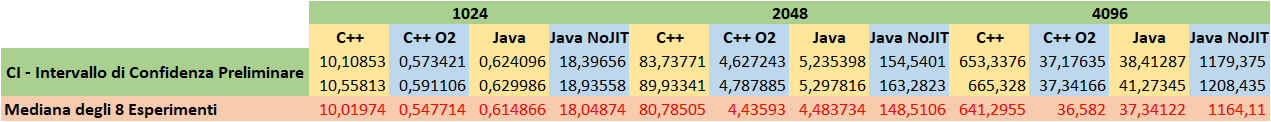
\includegraphics[width=1\linewidth,keepaspectratio]{CI_mediana}
  \caption{Intervalli di confidenza}
  \label{prodottomatrici_CI_mediana}
\end{figure}

Come si può osservare, che non tutte le medie calcolata sugli 8 esperimenti finali
rientrano nell'intervallo di confidenza calcolato sugli esperimenti effettuati
in fase preliminare.\\

\clearpage
\subsection{Validazione campioni}
Come detto in precedenza, si è deciso di utilizzare la mediana come indice di
tendenza centrale.\\
Per verificare la significatività dei campioni non è possibile applicare il
\textbf{T-Test}(valido nel caso in cui i campioni appartengono ad una Normale),
ma bisogna affidarsi a test non parametrici come il test di
\textbf{Wilcoxon/Kruskal-Wallis}.\\
Il test di Kruskal-Wallis, in particolare, serve a verificare se 2 o più campioni
indipendenti appartengono alla stessa popolazione.\\
Di seguito vengono mostrati i risultati ottenuti da JMP.\\

\begin{figure}[!htbp]
  \centering
  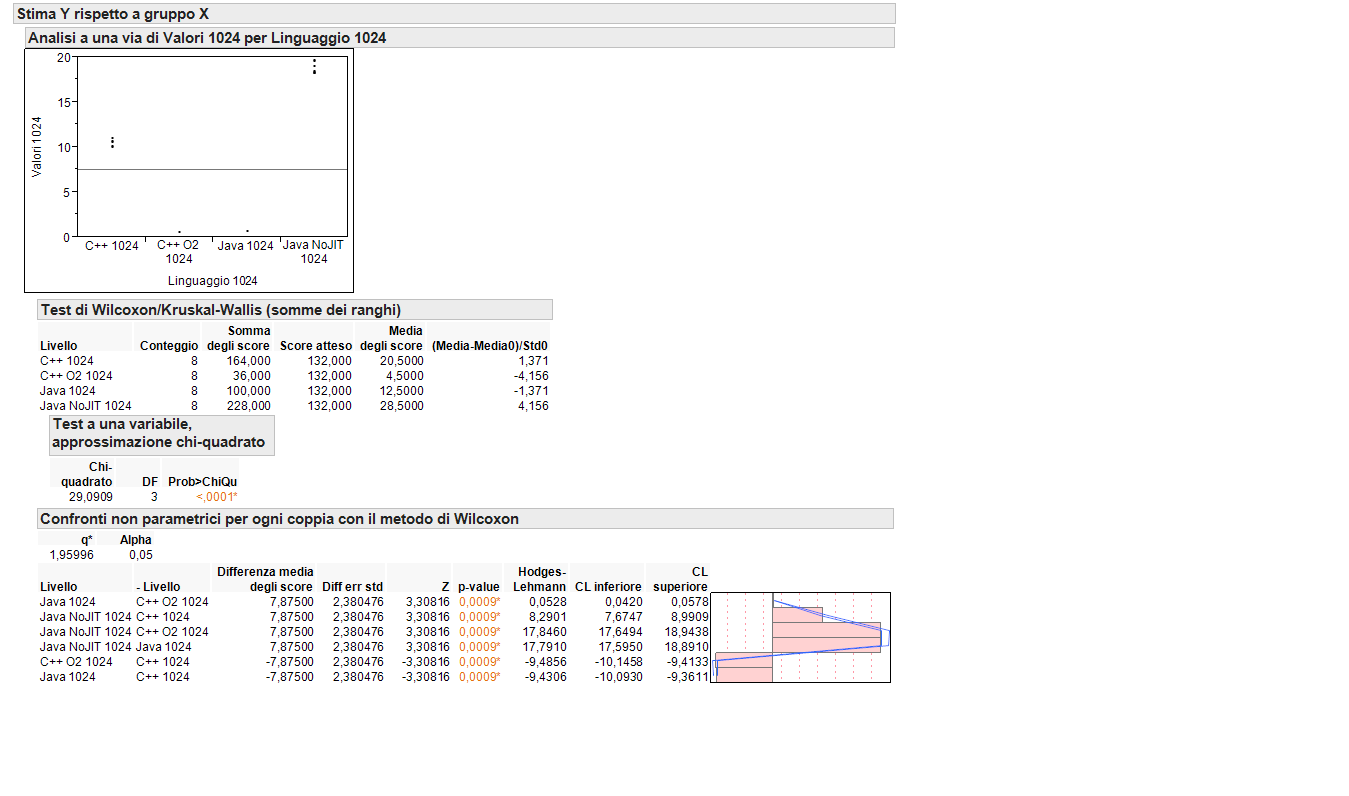
\includegraphics[width=1\linewidth,keepaspectratio]{Wilcoxon_Kruskal-Wallis_1024}
  \caption{Test di Wilcoxon/Kruskal-Wallis con matrici quadrate di dimensione 1024}
  \label{prodottomatrici_Wilcoxon_Kruskal-Wallis_1024}
\end{figure}

\clearpage

\begin{figure}[!htbp]
  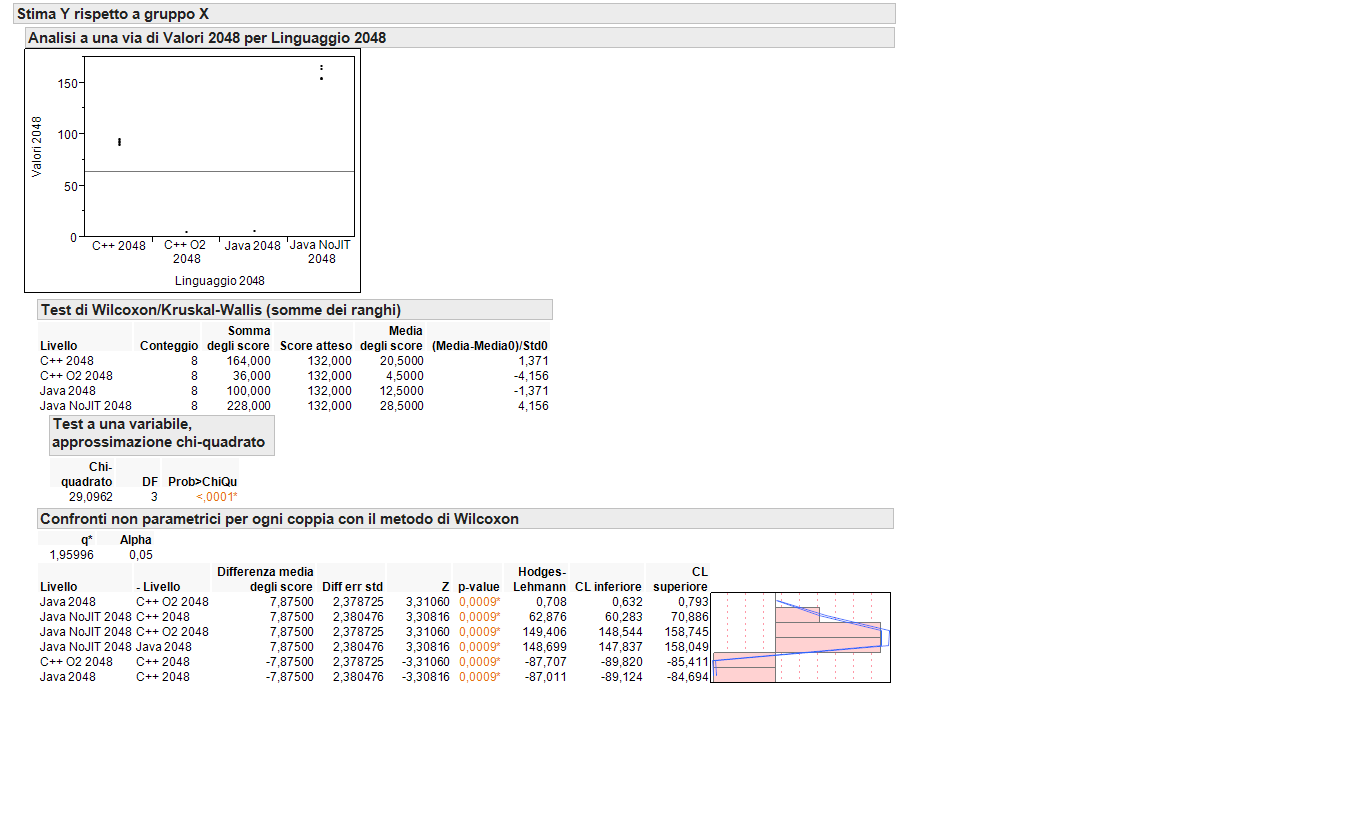
\includegraphics[width=1\linewidth,keepaspectratio]{Wilcoxon_Kruskal-Wallis_2048}
  \caption{Test di Wilcoxon/Kruskal-Wallis con matrici quadrate di dimensione 2048}
  \label{prodottomatrici_Wilcoxon_Kruskal-Wallis_2048}
\end{figure}

\clearpage

\begin{figure}[!htbp]
  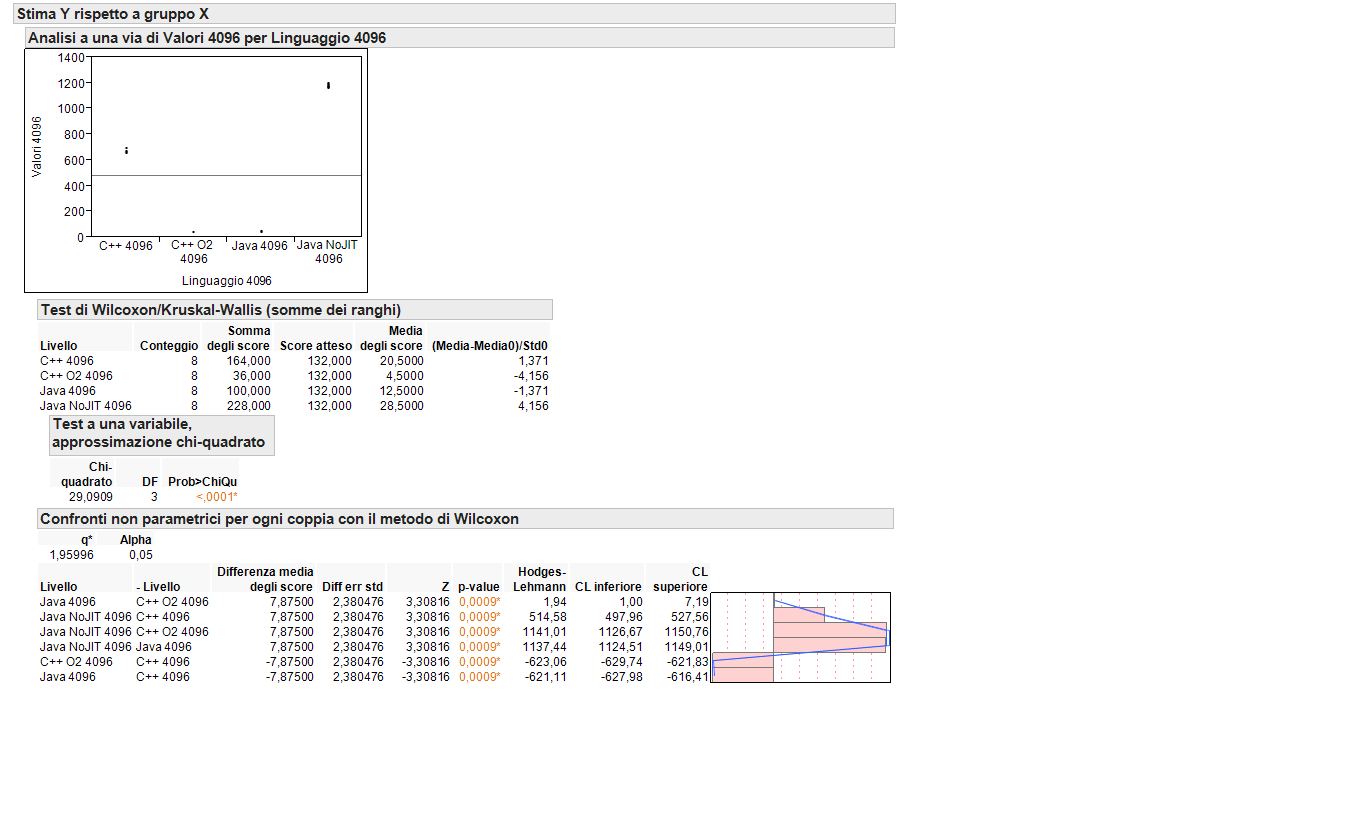
\includegraphics[width=1\linewidth,keepaspectratio]{Wilcoxon_Kruskal-Wallis_4096}
  \caption{Test di Wilcoxon/Kruskal-Wallis con matrici quadrate di dimensione 4096}
  \label{prodottomatrici_Wilcoxon_Kruskal-Wallis_4096}
\end{figure}

Tutti i test hanno portato alla stessa conclusione: l'ipotesi nulla è
rifiutata ($pvalue < 0.05$), di conseguenza i differenti gruppi non appartengono
alla stessa popolazione.\\

\clearpage

\section{Conclusioni}
Se si utilizzano ottimizzazioni configurabili dal compiler, in particolare O2
per C++ e il JIT in Java, il linguaggio di programmazione C++ risulta essere il
più veloce.\\
Tuttavia, disattivando ogni ottimizzazione dei compiler, il linguaggio C++
risulta essere comunque migliore di Java.\\
La supremazia del C++ discende dal fatto che è un linguaggio compilato ed
eseguito direttamente sulla macchina fisica, mentre il linguaggio Java è compilato
per ottenere un bytecode e poi interpretato ed eseguito sulla JVM, a sua volta
eseguita sulla macchina fisica.

\subsection{C++}
\subsubsection{Main}
\lstinputlisting[language=C++, caption={Codice C++}]{main.cpp}

\subsection{Java}
\subsubsection{MatrixMultiplicationù Class}
\lstinputlisting[language=Java, caption={Codice Java}]{MatrixMultiplication.java}
\subsubsection{Main}
\lstinputlisting[language=Java, caption={Codice Java}]{testMatrix.java}

\clearpage

\section{Script Batch}
Script per l'automazione degli esperimenti, al variare della
dimensione N, per tutti e quattro i casi(C++, Java, C++ O2, Java NoJIT).\\
\lstinputlisting[language=command.com, caption={Script Batch}]{script.bat}

\clearpage
Script per l'esecuzione nel particolare linguaggio scelto, per un numero
designato di volte, dell'algoritmo di Prodotto Matriciale.\\
\subsubsection{C++}
\lstinputlisting[language=command.com, caption={Script Batch}]{script_strassen_cpp.bat}
\subsubsection{Java}
\lstinputlisting[language=command.com, caption={Script Batch}]{script_strassen_java.bat}

	% !TEX root = ./main.tex
% !TEX encoding = UTF-8 Unicode
% !TEX program = pdflatex
% !TeX spellcheck = it_IT

\graphicspath{{Immagini/},{Immagini/pca_clustering/}}

\chapter{PCA \& Clustering}
Estrapolare un Workload sintetico a partire dal workload reale, riportato nel file
 \textit{PCA-CLASTERING-2017.jmp}.

\section{Obiettivo}
A partire dal workload reale, si vuole ottenere un \textbf{workload sintetico},
caratterizzato da un numero di osservazioni minori, che conservi quanta
più varianza possibile.

\section{Estrazione del Workload Sintetico}
Per estrarre il workload sintetico, dopo aver visionato i dati, si è scelto
di seguire il seguente procedimento:

\begin{itemize}
  \item Analisi del \textbf{\textit{CV(Coefficiente di Variazione)}}, per
  eliminare i parametri statisticamente non significativi;
  \item \textbf{\textit{PCA(Principal Component Analysis)}}, per ridurre il
  numero di parametri ed eliminare la correlazione tra essi;
  \item \textbf{\textit{Clustering}}, per ridurre il numero di esperimenti.
\end{itemize}


\subsection{Analisi del Coefficiente di Variazione}
In prima istanza, è stata effettuata un'analisi sul coefficiente di variazione(CV),
il quale esprime la dispersione dei valori dei singoli parametri attorno alla loro media.\\
Quando il coefficiente di variazione è nullo, il parametro
corrispondente non è statisticamente significativo e quindi è possibile eliminarlo.\\
Nella \figurename~\ref{cv} si evince l'assenza di colonne con coefficiente di variazione nullo,
quindi tutti i parametri dovranno essere utilizzati nelle successive fasi di analisi.

\begin{figure}[!htbp]
  \centering
	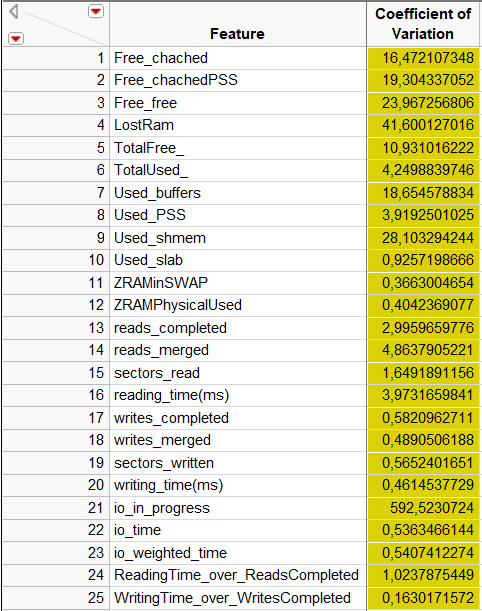
\includegraphics[width=.7\linewidth,keepaspectratio]{cov.png}
  \caption{Coefficiente di Variazione(CV)}
  \label{cv}
\end{figure}
\clearpage

\subsection{PCA}
In questa fase è stata applicata la
\textbf{\textit{PCA(Principal Component Analysis)}},
la quale trasforma un workload con parametri correlati in uno contenente parametri
incorrelati, ottenuti come combinazione lineare, pesata, di quelli iniziali.\\
L'utilizzo della PCA è fondamentale anche per la successiva fase di clustering, in
quanto quest'ultimo necessita che sia rispettata la proprietà di incorrelazione
dei parametri.\\
Per effettuare la PCA si è fatto utilizzo del tool statistico \textit{\textbf{JMP}}, nella
\figurename~\ref{pca} è riportato l'output.\\

\begin{figure}[!htbp]
	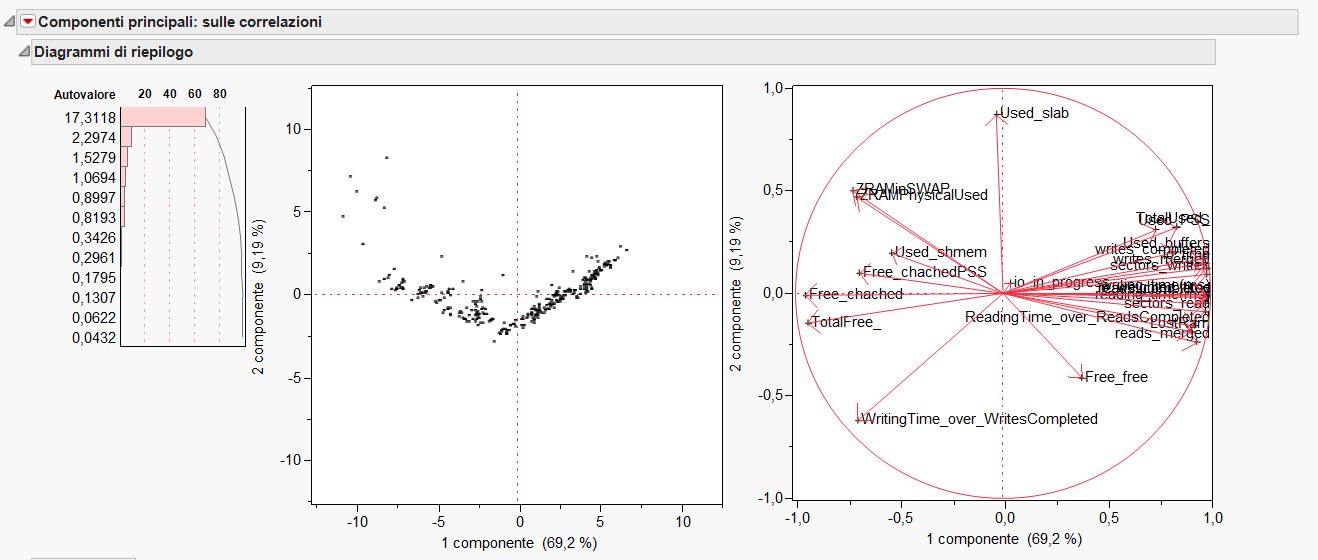
\includegraphics[width=\linewidth,keepaspectratio]{pca.png}
  \caption{Risultato PCA}
  \label{pca}
\end{figure}

\clearpage

Nella \figurename~\ref{autovalori} sono riportati gli autovalori ottenuti dalla PCA.\\

\begin{figure}[!htbp]
	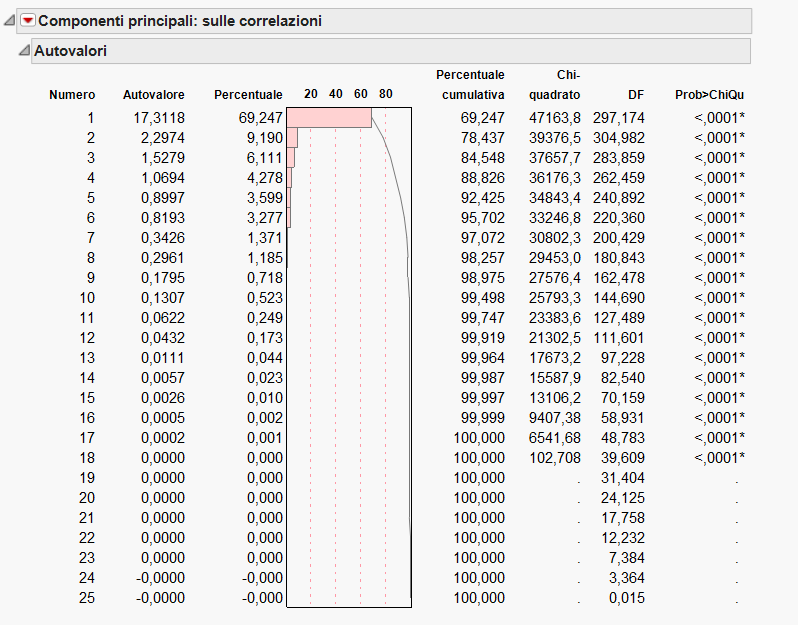
\includegraphics[width=\linewidth,keepaspectratio]{autovalori.png}
  \caption{Autovalori PCA}
  \label{autovalori}
\end{figure}

\clearpage

\begin{figure}[!htbp]
	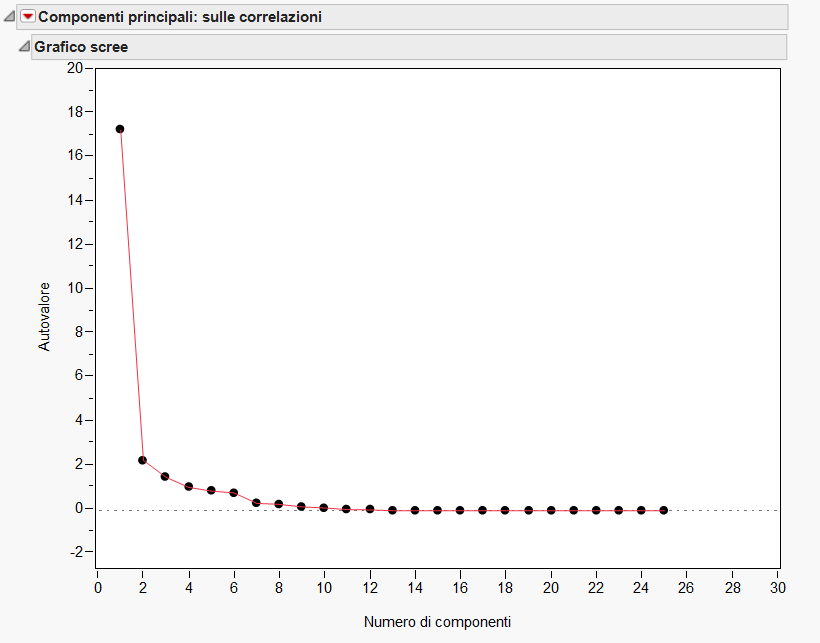
\includegraphics[width=\linewidth,keepaspectratio]{grafico_scree.png}
  \caption{Grafico Scree}
  \label{grafico_scree}
\end{figure}

\'E possibile scegliere il numero di componenti principali da utilizzare considerando
il ginocchio della curva ottenuta nella \figurename~\ref{grafico_scree}, rappresentante
sull'asse x il numero di componenti principali e sull'asse y
gli autovalori.\\
In questo caso, scegliendo di considerare 6 componenti principali, si è sicuri di conservare una quota di varianza sufficientemente
significativa(\textit{95,703\%}).\\
\clearpage
\begin{figure}[!htbp]
	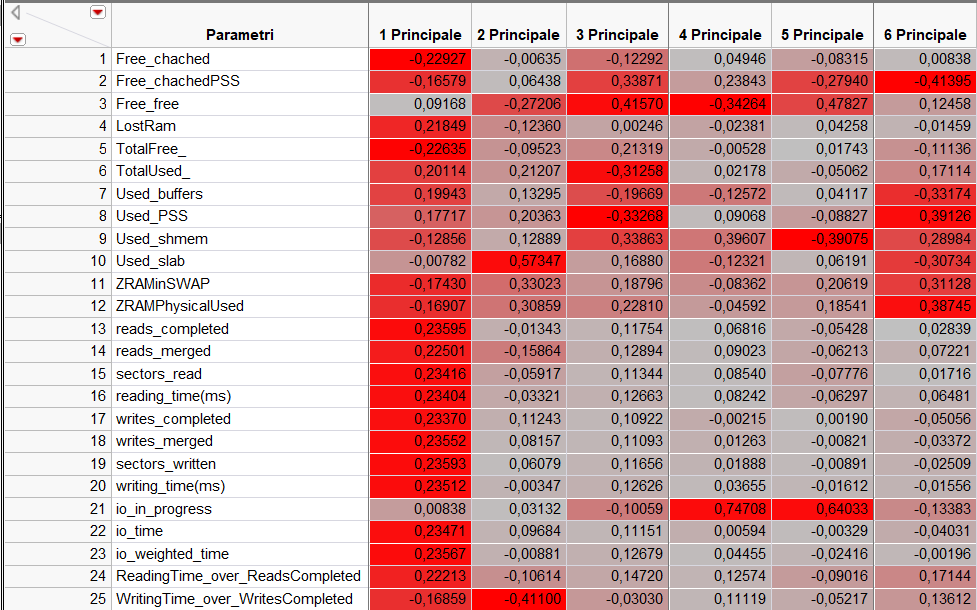
\includegraphics[width=\linewidth,keepaspectratio]{autovettori.png}
  \caption{Autovettori}
  \label{autovettori}
\end{figure}

Nella \figurename~\ref{autovettori} sono sfumati in rosso i parametri che
hanno contribuito maggiormente, in segno positivo o negativo, alla creazione
delle componenti principali scelte.\\
Valori vicini allo 0 indicano che quei parametri pesano relativamente poco nel
calcolo della componente principale.\\

% In particolare:
% \begin{itemize}
%   \item \textbf{\textit{Principale 1:}} \textit{Free\_chached, LostRam, TotalFree,
%   reads\_completed, reads\_merged, sectors\_read, reading\_time(ms),
%   writes\_completed, writes\_merged, sector\_written, writing\_time(ms),
%   io\_time, io\_weighted\_time e ReadingTime\_over\_ReadsCompleted};
%   \item \textbf{\textit{Principale 2:}} \textit{Used\_slab e WritingTime\_over\_WritesCompleted};
%   \item \textbf{\textit{Principale 3:}} \textit{Free\_free, TotalUsed e Used\_PSS};
%   \item \textbf{\textit{Principale 4:}} \textit{io\_in\_progress};
%   \item \textbf{\textit{Principale 5:}} \textit{Used\_shmem};autovettori
%   \item \textbf{\textit{Principale 6:}} \textit{Free\_chachedPSS, Used\_buffers e Used\_PSS, ZRamPhysicalUsed};
% \end{itemize}
\clearpage
\subsection{Clustering}
In questa fase è stato effettuata un'operazione di clustering sul risultato
ottenuto dallo step precedente.\\
La tecnica di clusterizzazione scelta è di tipo gerarchico agglomerativo,
in particolare è stata utilizzata la metrica di \textbf{Ward} per l'aggregazione
dei cluster.\\
Il criterio di Ward è diretto alla minimizzazione della varianza all’interno dei gruppi,
pertanto si presta bene ad essere utilizzato con variabili quantitative.\\
In \figurename~\ref{dendogramma} è riportato il dendogramma risultante.\\

\begin{figure}[!htbp]
	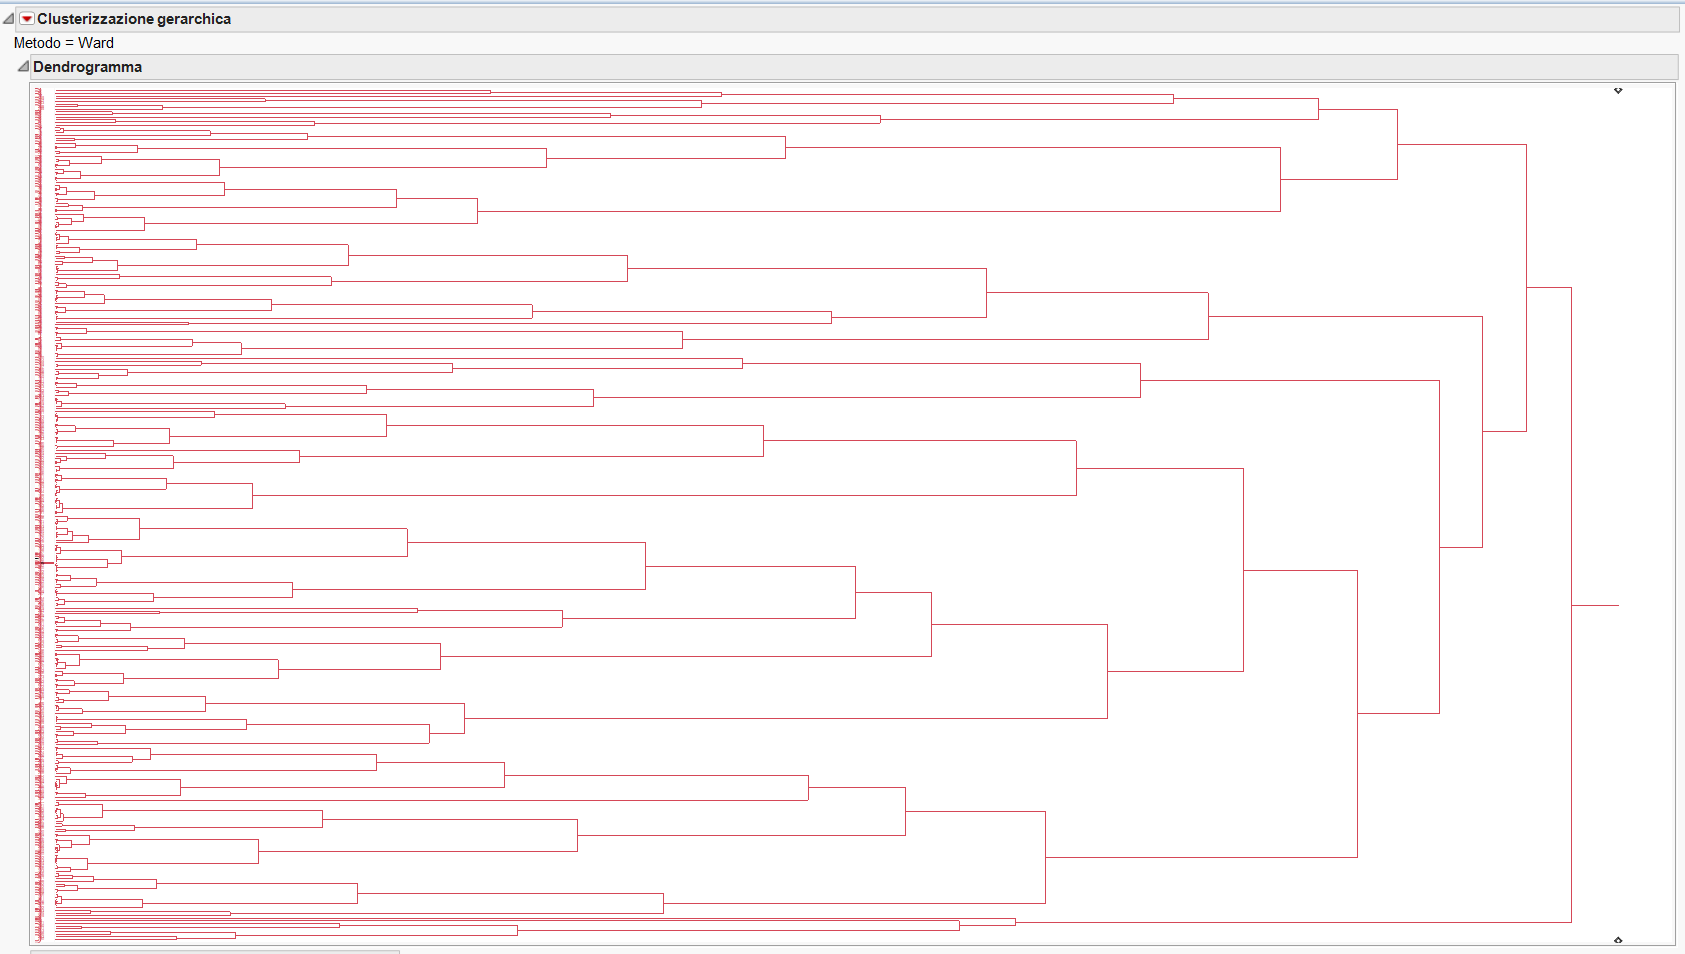
\includegraphics[width=\linewidth,keepaspectratio]{dendogramma.png}
  \caption{Dendogramma}
  \label{dendogramma}
\end{figure}
\clearpage
\begin{figure}[!htbp]
	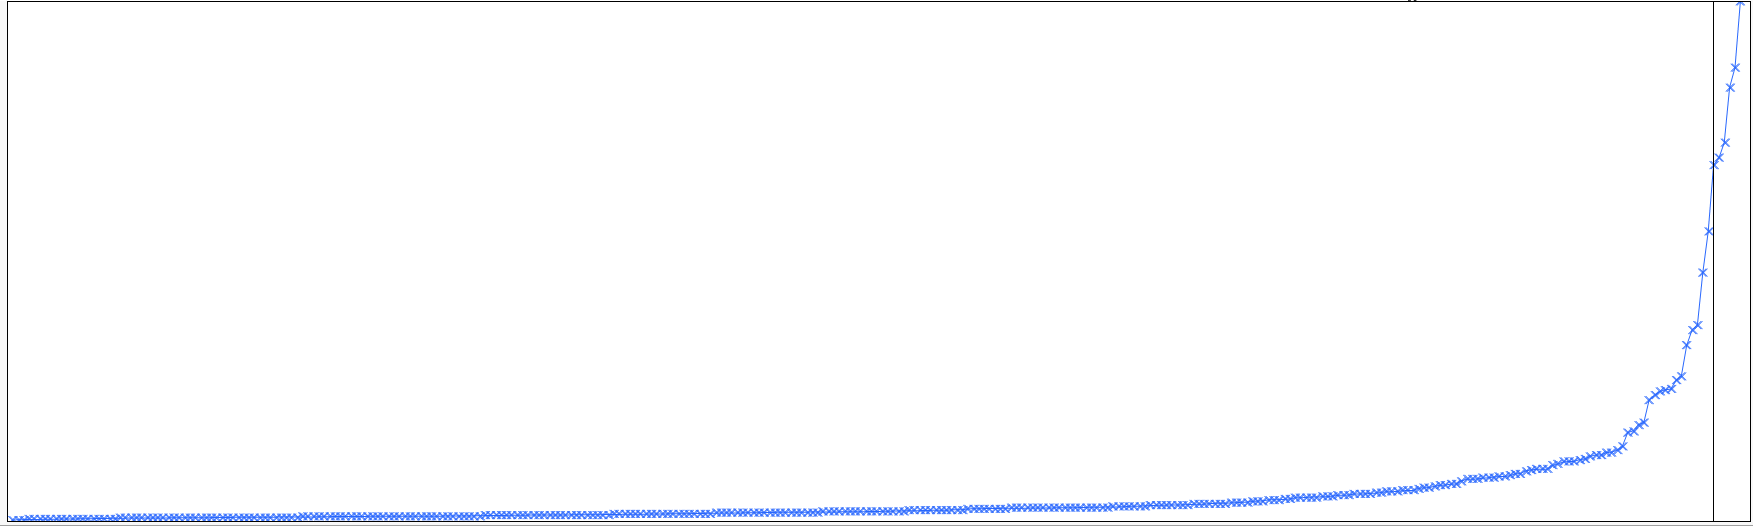
\includegraphics[width=\linewidth,keepaspectratio]{curva_dendogramma.png}
  \caption{Curva di Clustering}
  \label{curva_dendogramma}
\end{figure}

Facendo riferimento alla \figurename~\ref{curva_dendogramma}, è possibile scegliere
il numero di cluster posizionandosi nel ginocchio della curva, rappresentante le
distanze tra cluster.\\
In maniera analoga si può scegliere il numero di cluster utilizzando il criterio
di clusterizzazione cubica(\textbf{CCC}), riportato in \figurename~\ref{ccc},
scegliendo il numero di cluster in funzione della regola del massimo salto.\\

\begin{figure}[htbp]
\centering
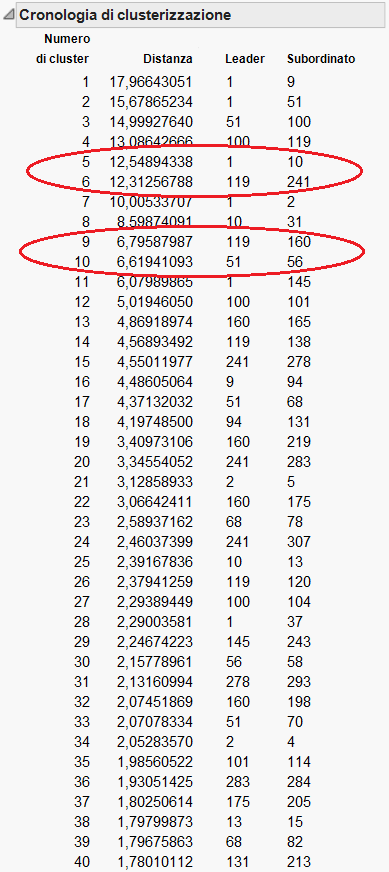
\includegraphics[width=50mm]{gerarchia_clustering.png}% "%" necessario
\qquad\qquad
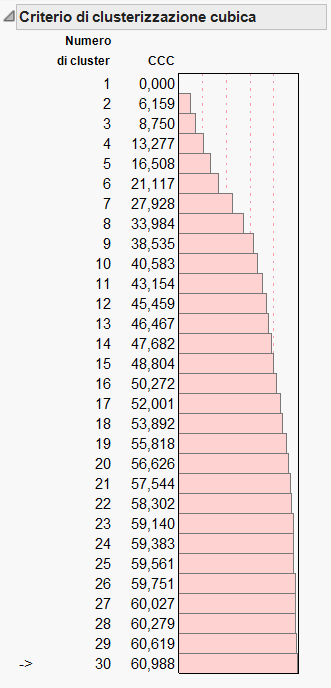
\includegraphics[width=50mm]{ccc.png}
\caption{Gerarchia Clustering e Criterio di Clusterizzazione Cubica}
\label{ccc}
\end{figure}

\clearpage

Sulla base dei criteri illustrati, si è scelto di considerare due soluzioni:
5 e 9 cluster.\\
Per generare i workload sintetici, inoltre, si è scelto di considerare il
centroide di ogni cluster.\\

\begin{figure}[!htbp]
	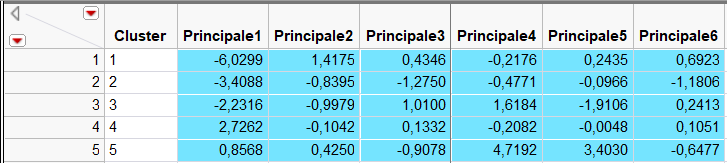
\includegraphics[width=\linewidth,keepaspectratio]{centroidi(5).png}
  \caption{Workload sintetico ottenuto con 5 cluster}
  \label{}
\end{figure}

\begin{figure}[!htbp]
	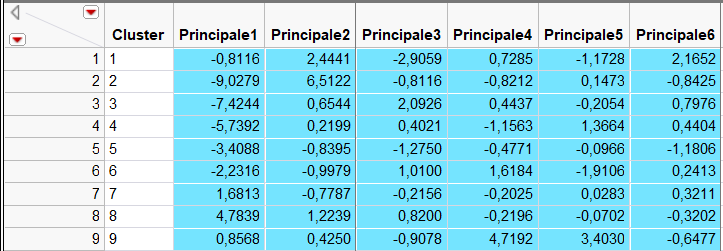
\includegraphics[width=\linewidth,keepaspectratio]{centroidi(9).png}
  \caption{Workload sintetico ottenuto con 9 cluster}
  \label{centroidi9}
\end{figure}

\clearpage
\section{Analisi}
Ottenuti i Workload Sintetici, è fondamentale osservare quanta varianza si è
conservata.\\
Per capire se la soluzione a 9 cluster è più conveniente della soluzione
a 5 cluster, bisogna confrontare la significatività conservata dai due workload sintetici.\\
Per fare ciò bisogna calcolare la varianza persa in ogni fase del processo di
caratterizzazione.\\
A valle della PCA, scegliendo solo 6 componenti principali, la varianza conservata
 risulta essere il 95,702\% della totale(valore ottenuto in JMP).\\
Per definire la significatività dei workload ottenuti con il clustering, invece, bisogna
utilizzare la devianza.\\
Quest'ultima è una grandezza indipendente dal grado di libertà, quindi si presta
perfettamente all'uso con i cluster, i quali hanno cardinalità differente.\\

La devianza del clustering è calcolata come la somma della devianza \textbf{inter-cluster}
e \textbf{intra-cluster}.\\
Tipicamente, per effettuare un buon clustering, si cerca di massimizzare la varianza
inter-clustering e minimizzare quella intra-clustering.\\
Nella seguente figura è riportata la devianza del workload sottoposto a PCA.\\

\begin{figure}[!htbp]
  \centering
	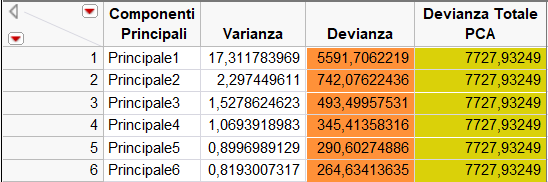
\includegraphics[width=.7\linewidth,keepaspectratio]{devianza_pca.png}
  \caption{Devianza PCA}
  \label{}
\end{figure}
\clearpage

\subsubsection{5 cluster}

Nella seguente figura è riportata la devianza inter-cluster.\\

\begin{figure}[!htbp]
  \centering
	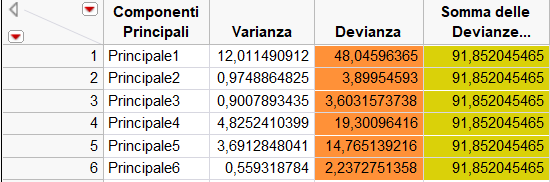
\includegraphics[width=.7\linewidth,keepaspectratio]{devianza_inter_clusters(5).png}
  \caption{Devianza Inter-Cluster}
  \label{}
\end{figure}

Nella seguente figura è riportata la devianza intra-cluster.\\

\begin{figure}[!htbp]
  \centering
	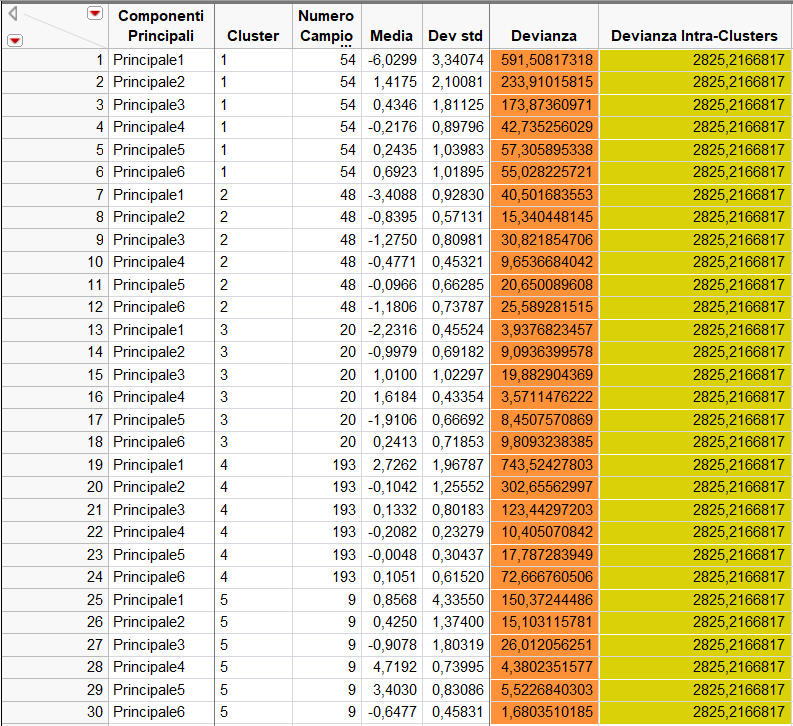
\includegraphics[width=.7\linewidth,keepaspectratio]{devianza_intra_clusters(5).png}
  \caption{Devianza Intra-Cluster}
  \label{}
\end{figure}
\clearpage

\subsubsection{9 cluster}

Nella seguente figura è riportata la devianza inter-cluster.\\

\begin{figure}[!htbp]
  \centering
	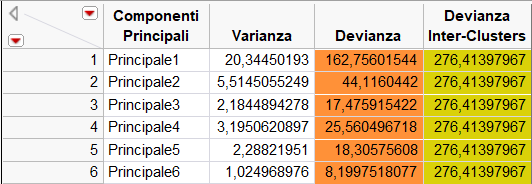
\includegraphics[width=.7\linewidth,keepaspectratio]{devianza_inter_clusters(9).png}
  \caption{Devianza Inter-Cluster}
  \label{}
\end{figure}

Nella seguente figura è riportata la devianza intra-cluster.\\

\begin{figure}[!htbp]
  \centering
	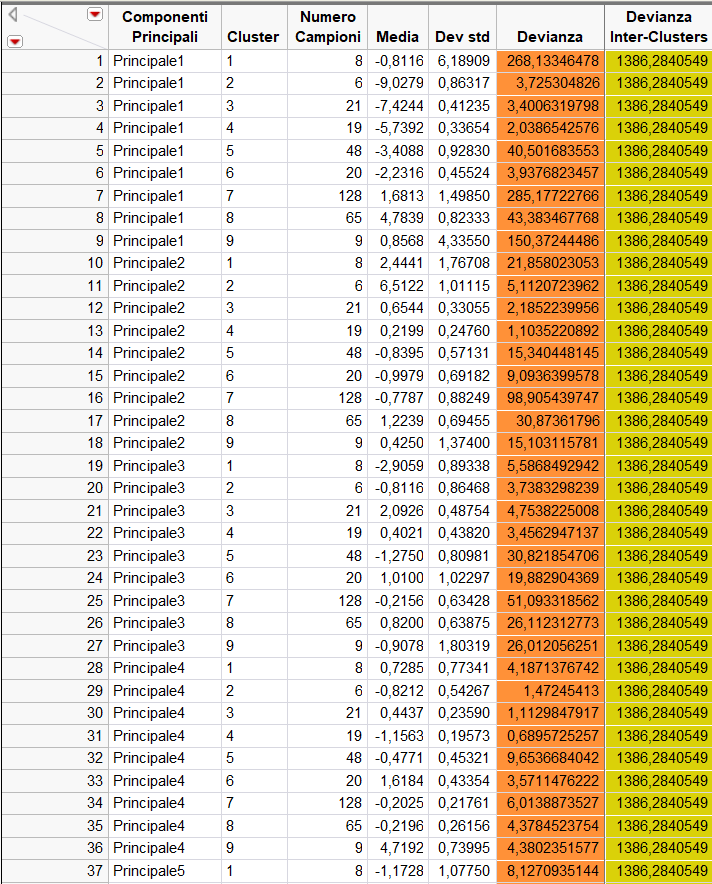
\includegraphics[width=.5\linewidth,keepaspectratio]{devianza_intra_clusters(9).png}
  \caption{Devianza Intra-Cluster}
  \label{}
\end{figure}
\clearpage
\section{Conclusioni}

Dopo aver ottenuto i valori di devianza del workload sottoposto a PCA e, successivamente,
a Clustering, considerando 5 e 9 cluster, è possibile calcolarne la significatività.\\
La devianza conservata utilizzando la tecnica di clustering si calcola con la
seguente formula:
$$1-{devianza_{inter\_cluster}+devianza_{intra\_cluster}\over {devianza_{pca}}}$$

Nelle seguenti Tabelle sono riportate le percentuali di devianza persa e conservata,
 nei due casi analizzati.\\
\vspace{5 mm}

\begin{center}
  \textbf{5 Cluster}
\end{center}
\begin{figure}[!htbp]
  \centering
  \begin{tabular}{|c|c|}
  \hline
  \textbf{Devianza PCA}	& 7727,93249 \\
  \hline
  \textbf{Devianza Clustering(intra-cluster+inter-cluster)}	& 2917,0687 \\
  \hline
  \textbf{Percentuale devianza persa con il clustering}	& 37,75\% \\
  \hline
  \textbf{Percentuale devianza conservata con il clustering}	& 62,25\% \\
  \hline
  \textbf{Significatività PCA} &	95,70\% \\
  \hline
  \end{tabular}
  %\caption{Workload con 5 cluster}
\end{figure}


\vspace{5 mm}
\begin{center}
  \textbf{9 Cluster}
\end{center}
\begin{figure}[!htbp]
  \centering
  \begin{tabular}{|c|c|}
    \hline
    \textbf{Devianza PCA}	& 7727,93249 \\
    \hline
    \textbf{Devianza Clustering(intra-cluster+inter-cluster)}	& 1662,6980 \\
    \hline
    \textbf{Percentuale devianza persa con il clustering}	& 21,52\% \\
    \hline
    \textbf{Percentuale devianza conservata con il clustering}	& 78,48\% \\
    \hline
    \textbf{Significatività PCA} &	95,70\% \\
    \hline
  \end{tabular}
  %\caption{Workload con 9 cluster}
\end{figure}

\clearpage

In seguito sono riportate le tabelle che riassumono la significatività perduta e
conservata a partire dal Workload Reale fino a quello Sintetico, ottenuto con
PCA e Clustering.\\

\vspace{5 mm}
\begin{center}
  \textbf{5 Cluster}
\end{center}
\begin{figure}[!htbp]
  \centering
  \begin{tabular}{c|c|c}
   & \textbf{Conservata} & \textbf{Perse} \\
   \hline
   \textbf{Workload Reale} & 100,00\% &	0,00\% \\
   \hline
   \textbf{PCA} &	95,70\%	& 4,30\% \\
   \hline
   \textbf{Clustering} &	59,58\%	& 40,42\% \\
  \end{tabular}
  % \caption{Significatività Workload con 5 cluster}
\end{figure}

\vspace{5 mm}
\begin{center}
  \textbf{9 Cluster}
\end{center}
\begin{figure}[!htbp]
  \centering
  \begin{tabular}{c|c|c}
   & \textbf{Conservata} & \textbf{Persa} \\
   \hline
   \textbf{Workload Reale} & 100,00\% &	0,00\% \\
   \hline
   \textbf{PCA} &	95,70\%	& 4,30\% \\
   \hline
   \textbf{Clustering} &	75,11\%	& 24,89\% \\
  \end{tabular}
  % \caption{Significatività Workload con 9 cluster}
\end{figure}

\vspace{5 mm}

In conclusione, utilizzando 6 componenti principali e 5 cluster, si perde il 40,42\%
di significatività rispetto al workload reale mentre scegliendo 9 cluster si perde il 24,89\%.\\
La percentuale di varianza conservata considerando 9 cluster è notevolmente maggiore,
con il compromesso di dover effettuare 9 esperimenti.\\
Quindi si può affermare che, se non ci sono particolari limitazioni di costo e/o tempo,
il workload sintetico con 9 cluster rappresenta una soluzione migliore.\\
Per sottoporre il Workload Sintetico al sistema da testare è necessario identificare
quali sono i parametri del Workload Reale che contribuiscono maggiormente
alla formazione delle componenti principali utilizzate.\\
Tale operazione si effettua considerando la matrice degli autovettori, riportata
in \figurename~\ref{autovettori}, e scegliendo solo i quattro parametri con maggior
peso, due negativi e due positivi, per ogni PC.\\
Successivamente, in accordo con il segno del valori rispetto ad ogni componente
principale, presenti in \figurename~\ref{centroidi9}, si caratterizzano i
differenti cluster o con i due parametri positivi scelti o con i due negativi.\\
In tabella è riportato il risultato ottenuto.
\begin{figure}
\centering
   \begin{tabular}{p{0.1\linewidth} || p{0.4\linewidth} | p{0.55\linewidth}}
     \textbf{Cluster} & \textbf{Principale 1} & \textbf{Principale 2} \\
     \hline
     \hline
     \textbf{1} & \textit{Free\_cached, TotalFree\_} & \textit{Used\_slab, ZRAMinSWAP} \\
     \hline
     \textbf{2} & \textit{Free\_cached, TotalFree\_} & \textit{Used\_slab, ZRAMinSWAP} \\
     \hline
     \textbf{3} & \textit{Free\_cached, TotalFree\_} & \textit{Used\_slab, ZRAMinSWAP} \\
     \hline
     \textbf{4} & \textit{Free\_cached, TotalFree\_} & \textit{Used\_slab, ZRAMinSWAP} \\
     \hline
     \textbf{5} & \textit{Free\_cached, TotalFree\_} & \textit{WritingTime\_over\_WritesCompleted, Free\_free} \\
     \hline
     \textbf{6} & \textit{Free\_cached, TotalFree\_} & \textit{WritingTime\_over\_WritesCompleted, Free\_free} \\
     \hline
     \textbf{7} & \textit{reads\_completed, sectors\_written} &	\textit{WritingTime\_over\_WritesCompleted, Free\_free} \\
     \hline
     \textbf{8} &  \textit{reads\_completed, sectors\_written} & \textit{Used\_slab, ZRAMinSWAP} \\
     \hline
     \textbf{9} &  \textit{reads\_completed, sectors\_written} & \textit{Used\_slab, ZRAMinSWAP} \\
     \hline
   \end{tabular}
  \begin{tabular}{p{0.1\linewidth} || p{0.4\linewidth} | p{0.55\linewidth}}
   & \textbf{Principale 3} & \textbf{Principale 4}  \\
    \hline
    \hline
    \textbf{1} & \textit{Used\_PSS, TotalUsed\_} & \textit{io\_in\_progress, Used\_shmem} \\
    \hline
    \textbf{2} & \textit{Used\_PSS, TotalUsed\_} & \textit{Free\_free, Used\_buffers} \\
    \hline
    \textbf{3} & \textit{Free\_free, Free\_chachedPSS} & \textit{io\_in\_progress, Used\_shmem} \\
    \hline
    \textbf{4} & \textit{Free\_free, Free\_chachedPSS} & \textit{Free\_free, Used\_buffers} \\
    \hline
    \textbf{5} & \textit{Used\_PSS, TotalUsed\_}  & \textit{Free\_free, Used\_buffers} \\
    \hline
    \textbf{6} & \textit{Free\_free, Free\_chachedPSS} & \textit{io\_in\_progress, Used\_shmem} \\
    \hline
    \textbf{7} & \textit{Used\_PSS, TotalUsed\_}  & \textit{Free\_free, Used\_buffers} \\
    \hline
    \textbf{8} & \textit{Free\_free, Free\_chachedPSS} & \textit{Free\_free, Used\_buffers} \\
    \hline
    \textbf{9} & \textit{Used\_PSS, TotalUsed\_} & \textit{io\_in\_progress, Used\_shmem} \\
    \hline
  \end{tabular}
  \begin{tabular}{p{0.1\linewidth} || p{0.4\linewidth} | p{0.55\linewidth}}
    & \textbf{Principale 5} & \textbf{Principale 6}  \\
   \hline
   \hline
   \textbf{1} & \textit{Used\_shmem, Free\_chachedPSS} & \textit{Used\_PSS, ZRAMPhysicalUsed} \\
   \hline
   \textbf{2} & \textit{io\_in\_progress, Free\_free} & \textit{Free\_chachedPSS, Used\_buffers} \\
   \hline
   \textbf{3} & \textit{Used\_shmem, Free\_chachedPSS} & \textit{Used\_PSS, ZRAMPhysicalUsed} \\
   \hline
   \textbf{4} & \textit{io\_in\_progress, Free\_free} & \textit{Used\_PSS, ZRAMPhysicalUsed} \\
   \hline
   \textbf{5} & \textit{Used\_shmem, Free\_chachedPSS} & \textit{Free\_chachedPSS, Used\_buffers} \\
   \hline
   \textbf{6} & \textit{Used\_shmem, Free\_chachedPSS} & \textit{Used\_PSS, ZRAMPhysicalUsed} \\
   \hline
   \textbf{7} & \textit{io\_in\_progress, Free\_free} & \textit{Used\_PSS, ZRAMPhysicalUsed} \\
   \hline
   \textbf{8} & \textit{Used\_shmem, Free\_chachedPSS} & \textit{Free\_chachedPSS, Used\_buffers} \\
   \hline
   \textbf{9} & \textit{io\_in\_progress, Free\_free} & \textit{Free\_chachedPSS, Used\_buffers} \\
   \hline
  \end{tabular}
  \caption{Parametri Caratterizzanti il Workload Sintetico con 9 cluster}
  \end{figure}

	% !TEX root = ./main.tex
% !TEX encoding = UTF-8 Unicode
% !TEX program = pdflatex
% !TeX spellcheck = it_IT

\graphicspath{{Immagini/},{Immagini/webServer/}}

\chapter{Web Server}

\section{Traccia}
Emulare un Web Server Apache ed un set di utenti che richiedono delle risorse.
Monitorare il workload osservato, successivamente caratterizzarlo ed effettuare
un'analisi di performance.\\

\section{Piattaforma}
\subsubsection*{Client}
Il client su cui è stato eseguito \textbf{JMeter}(un generatore di workload), è
un notebook MSI con le seguenti caratteristiche:

\begin{itemize}
  \item \textbf{Processore}: Intel(R) Core(TM) i7-7700HQ @ 2.80GHz
  \item \textbf{Memoria Ram}: 16GB DDR4-2400MHz
  \item \textbf{Tipo sistema}: Windows 10 64bit, processore basato su x64
  \item \textbf{Storage}: SSD Kingston M.2.SATA 480GB
\end{itemize}

\subsubsection*{Server}

Il Web Server Apache è stato installato su un notebook Asus con le seguenti
caratteristiche:

\begin{itemize}
  \item \textbf{Processore}: Intel(R) Core(TM) Pentium
  \item \textbf{Memoria Ram}: 4GB DDR3-1600MHz
  \item \textbf{Tipo sistema}: Ubuntu 16.4 LTS, processore basato su x64
  \item \textbf{Storage}: SSD Samsung 850 EVO SATA 3
\end{itemize}

La connessione Client-Server è stata effettuata in modo diretto tramite un
cavo ethernet.\\

\section{Caratterizzazione Workload}
Per caratterizzare il Workload sono state simulate richieste HTTP random al server,
teli richieste sono state effettuate su 6 pagine html.\\
Le pagine differiscono per dimensione e per tipologia:

\begin{itemize}
  \item Dimensione
  \begin{itemize}
    \item \textbf{\textit{Piccole}}: dell'ordine delle decine di KB;
    \item \textbf{\textit{Medie}}: dell'ordine delle centinaia di KB;
    \item \textbf{\textit{Grandi}}: dell'ordine delle migliaia di KB;
  \end{itemize}
  \item Tipologia
  \begin{itemize}
    \item \textbf{\textit{Testo}};
    \item \textbf{\textit{Immagine}}.
  \end{itemize}
\end{itemize}

Lato Client, i dati sono stati collezionati con il tool \textbf{Jmeter}, configurando
un \textit{Test Plan} opportuno.\\
Lato Server, invece, i dati sono stati collezionati con il tool \textbf{collectl}
di Linux.\\
Il numero di pagine, la dimensione ed il numero di Thread Groups scelti per la
caratterizzazione del workload sono frutto di un'attenta analisi preliminare.\\

\subsection{Problematica Saturazione Server}
Durante gli esperimenti preliminari sostenuti per comprendere al meglio gli strumenti
e i parametri a disposizione, si è giunti alla conclusione che non è possibile,
utilizzando una sola macchina client, saturare al meglio la macchina server.\\
Infatti, in conclusione ai test effettuati, si è dedotto che, prima di riuscire
a saturare le risorse hardware del server, quali CPU e RAM, il collo di bottiglia
è rappresentato dall'infrastruttura di rete.\\
In particolare, il comportamento evidenziatosi è dovuto alla mancata risposta
del Server a tutte le sollecitazioni prodotte dal Client, nonostante
il monitoraggio delle risorse del primo mostrasse di essere ben lontano
dalla sua soglia massima di capacità servente.\\
Nelle seguenti figure sono riportati i report degli esperimenti svolti in JMeter
ed il monitoraggio delle risorse del server, al variare del numero di Thread Group
istanziati.\\

\subsubsection{Esperimento con 10 Thread Group}
\begin{minipage}{\linewidth}
  \centering
  \begin{minipage}{1\linewidth}
    \begin{figure}[H]
      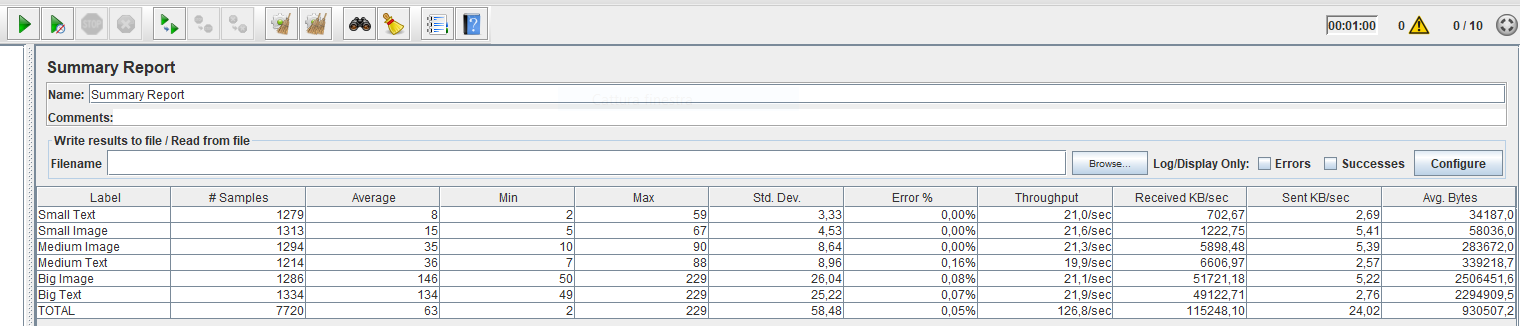
\includegraphics[width=\linewidth]{jmeter_analisi_10thread}
    \end{figure}
  \end{minipage}
  \begin{minipage}{1\linewidth}
    \begin{figure}[H]
      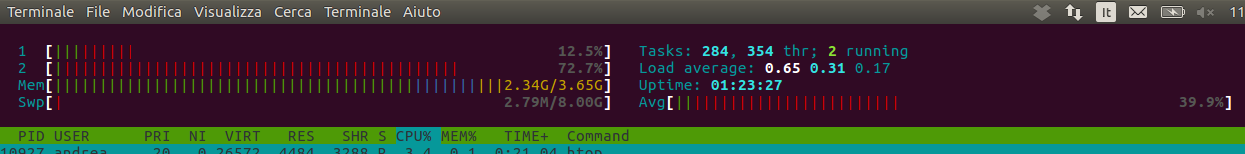
\includegraphics[width=\linewidth]{100_thread_server}
    \end{figure}
  \end{minipage}
\end{minipage}

\subsubsection{Esperimento con 100 Thread Group}
\begin{minipage}{\linewidth}
  \centering
  \begin{minipage}{1\linewidth}
    \begin{figure}[H]
      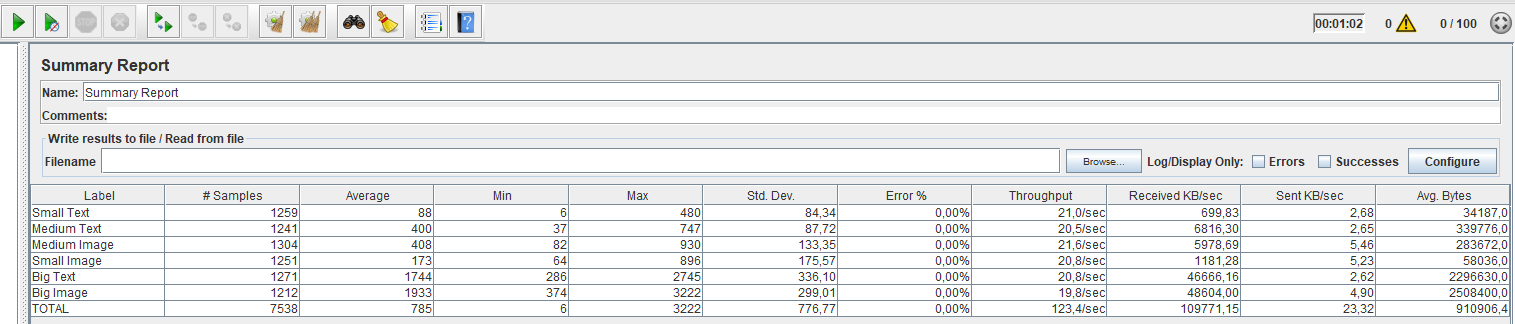
\includegraphics[width=\linewidth]{jmeter_analisi_100thread}
    \end{figure}
  \end{minipage}
  \begin{minipage}{1\linewidth}
    \begin{figure}[H]
      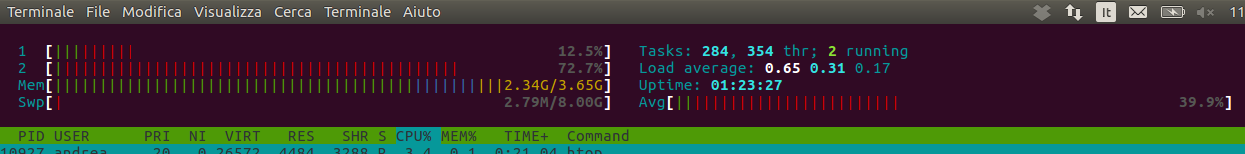
\includegraphics[width=\linewidth]{100_thread_server}
    \end{figure}
  \end{minipage}
\end{minipage}

\subsubsection{Esperimento con 500 Thread Group}
\begin{minipage}{\linewidth}
  \centering
  \begin{minipage}{1\linewidth}
    \begin{figure}[H]
      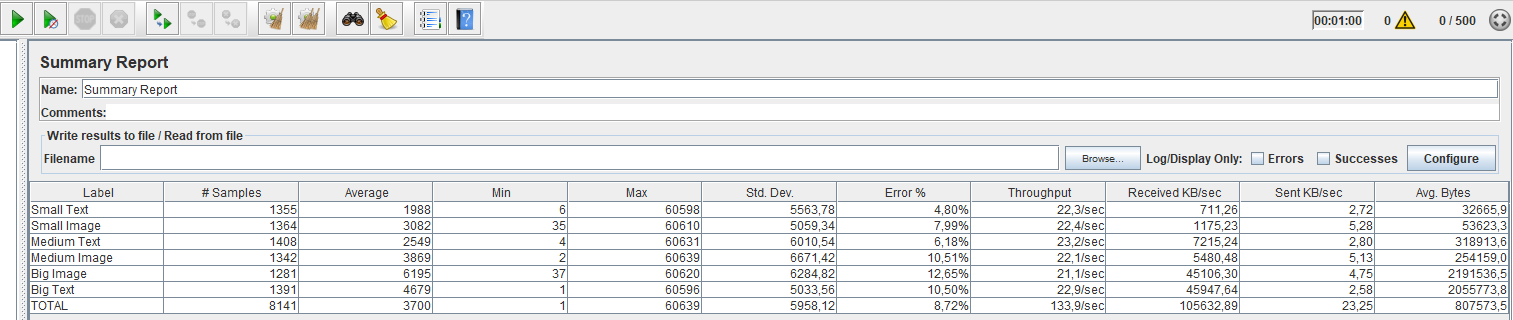
\includegraphics[width=\linewidth]{jmeter_analisi_500thread}
    \end{figure}
  \end{minipage}
  \begin{minipage}{1\linewidth}
    \begin{figure}[H]
      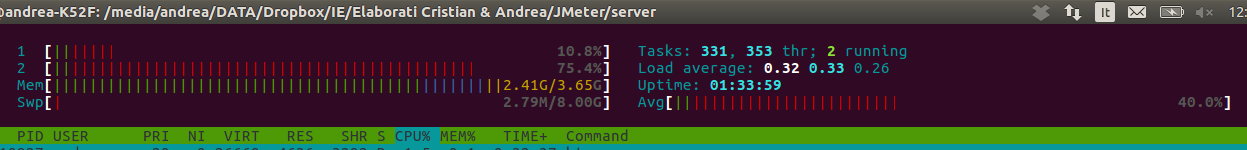
\includegraphics[width=\linewidth]{500_thread_server}
    \end{figure}
  \end{minipage}
\end{minipage}

\subsubsection{Esperimento con 1000 Thread Group}
\begin{minipage}{\linewidth}
  \centering
  \begin{minipage}{1\linewidth}
    \begin{figure}[H]
      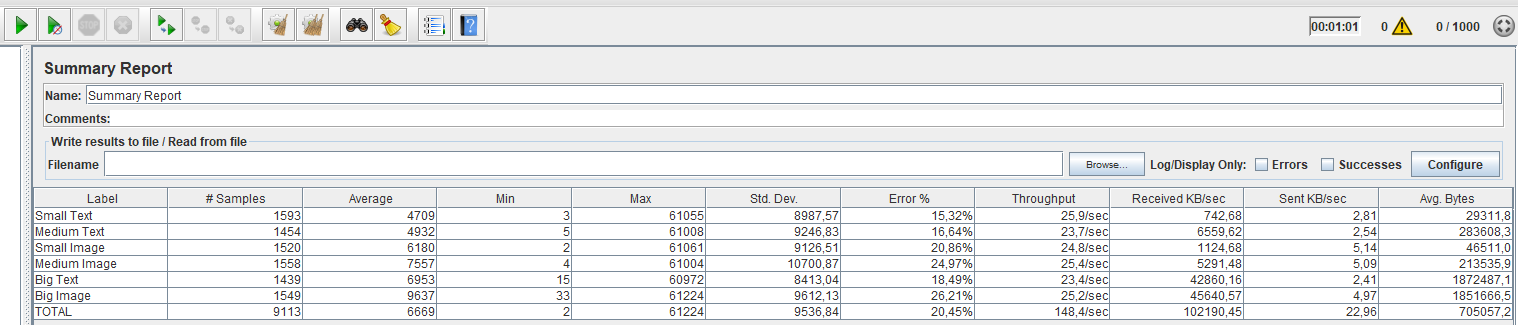
\includegraphics[width=\linewidth]{jmeter_analisi_1000thread}
    \end{figure}
  \end{minipage}
  \begin{minipage}{1\linewidth}
    \begin{figure}[H]
      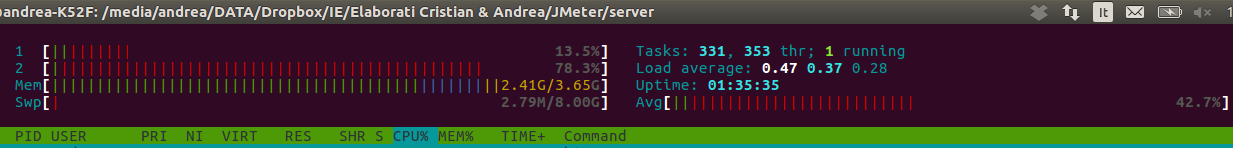
\includegraphics[width=\linewidth]{1000_thread_server}
    \end{figure}
  \end{minipage}
\end{minipage}

\vspace{1cm}
Il parametro Thread Group indica il numero di clients che effettuano continuamente
richieste HTTP al server.\\
Ovviamente questo numero di Threads è simulato dall'unica macchina client utilizzata,
tramite il tool JMeter.\\
Come si può osservare dalle immagini riportate, essendoci una sola macchina fisica,
al crescere del numero di richieste aumenta il numero di errori.\\
Questi errori però non sono da individuare nell'incapacità del server di gestire
la mole di richieste(infatti la CPU è mediamente occupata a circa il 40\% mentre
la RAM al 65\%), bensì nell'infrastruttura di rete(scheda di rete e cavo Ethernet),
limitata ad \textbf{1Gb/s}.\\

In \figurename~\ref{webserver_bottleneck_rete} è riportato l'utilizzo dell'I/O di rete,
raffigurante, in alcuni punti, il raggiungimento del limite fisico(1Gb/s).\\
\begin{figure}[!htbp]
  \centering
  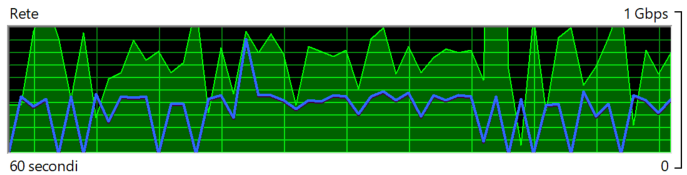
\includegraphics[width=1\linewidth, keepaspectratio]{client_rete_bottleneck}
  \caption{Infrastruttura di Rete - Bottleneck}
  \label{webserver_bottleneck_rete}
\end{figure}

\clearpage

\subsection{Analisi Alto Livello (Client)}
\subsubsection*{Impostazioni Client (JMeter)}
Prima di effettuare gli esperimenti, è stato necessario configurare alcuni parametri
nel Test Plan di JMeter, riportati in \figurename~\ref{webserver_conf_jmeter}

\begin{figure}[!htbp]
  \centering
  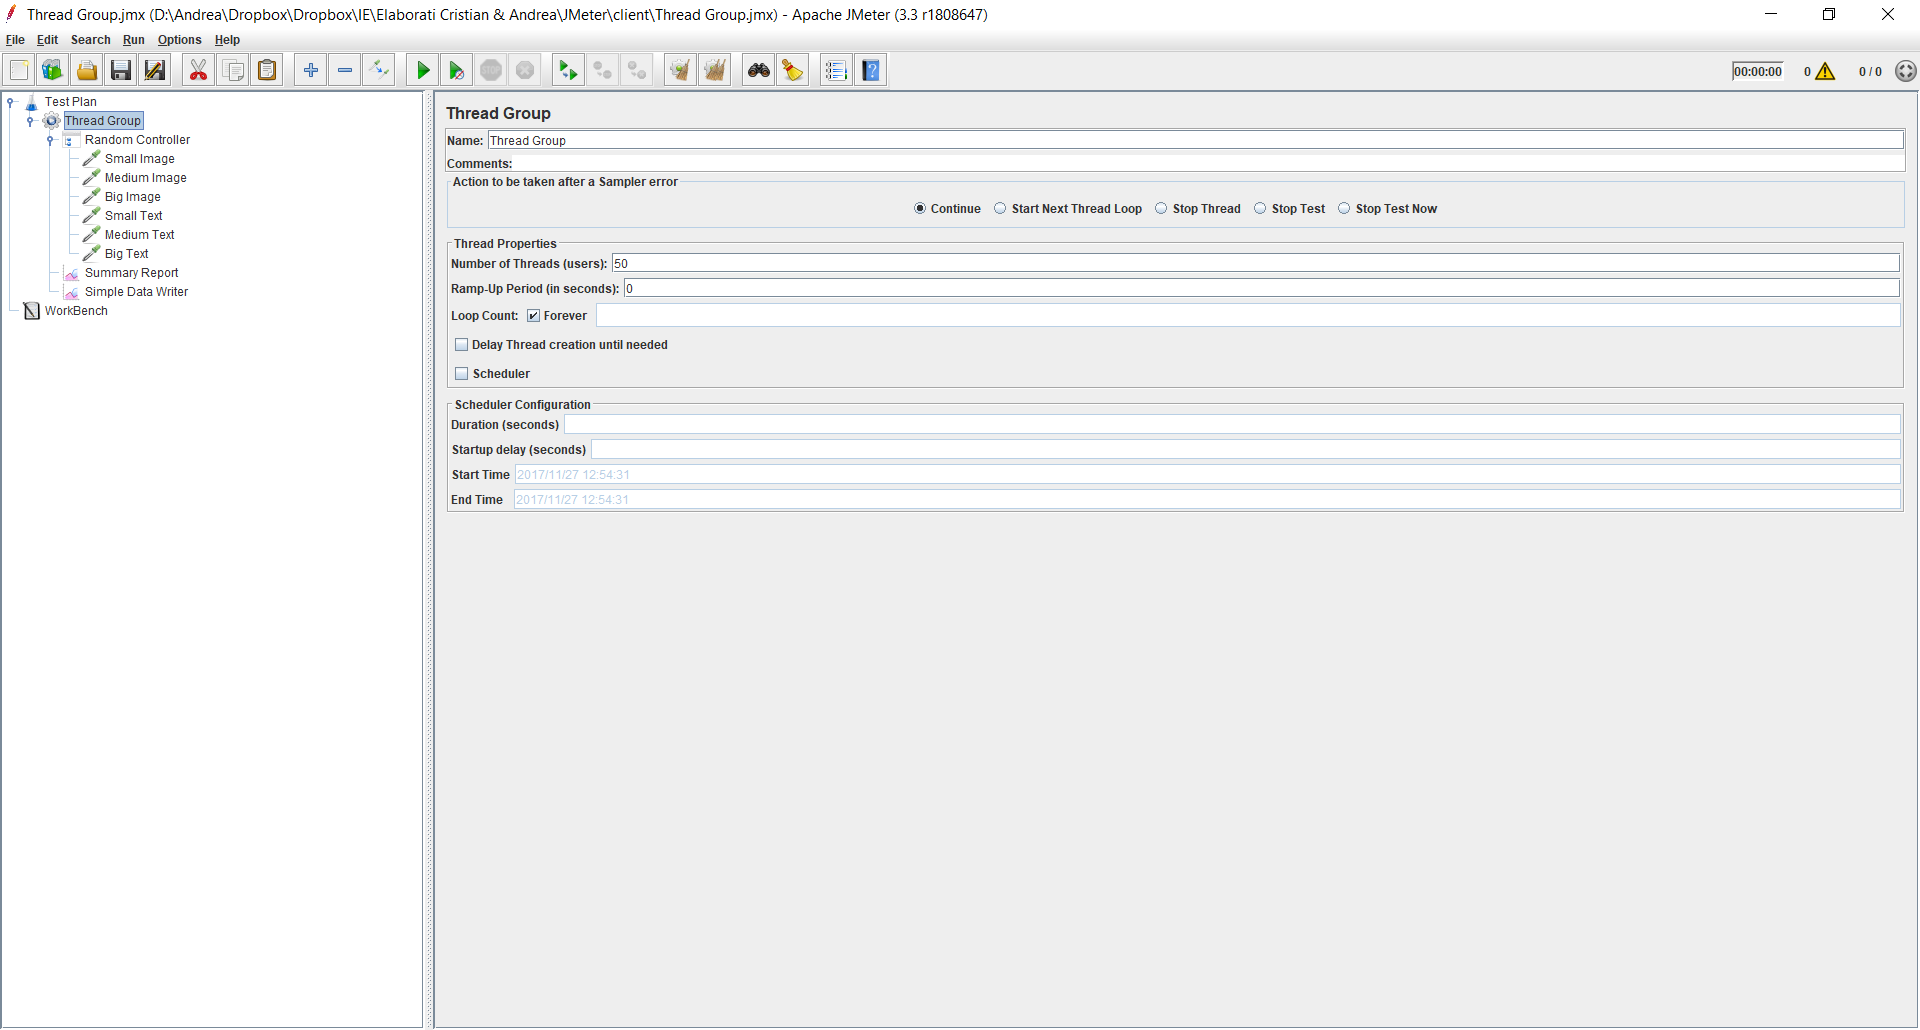
\includegraphics[width=1\linewidth, keepaspectratio]{conf_thread_group}
  \caption{}
  \label{webserver_conf_jmeter}
\end{figure}

In particolare, si evince che il Test Plan è stato caratterizzato dai seguenti
componenti:

\begin{itemize}
  \item \textbf{\textit{Random Controller}} - per generare richieste tra le possibili
  pagine in maniera randomica ed uniforme;
  \item \textbf{\textit{HTTP Request}} - una per pagina, serve per generare una
  richiesta HTTP;
  \item \textbf{\textit{Summary Report}} - genera un report immediato degli esperimenti
  in esecuzione.
  \item \textbf{\textit{Simple Data Writer}} - scrive i risultati degli esperimenti
  in un file .csv
\end{itemize}

JMeter è stato configurato attivando il \textbf{Keep Alive} ad ogni pagina
ed il parametro \textbf{Retrieve All Embedded Resources}(necessario per prelevare
le immagini linkate nell'html).\\
Nonostante gli esperimenti siano stati eseguiti per un tempo di 8 minuti, è stato
effettuato un filtraggio dei dati del primo ed ultimo minuto di esecuzione, al fine
di eliminare eventuali comportamenti transitivi.\\

I parametri utilizzati per la caratterizzazione del workload lato client sono:
\textbf{Latency}, \textbf{Elapsed Time}, \textbf{Bytes}.\\

In \figurename~\ref{webserver_distribuzioni_parametri} sono riportate le distribuzioni dei
tre parametri.\\

\begin{figure}[!htbp]
  \centering
  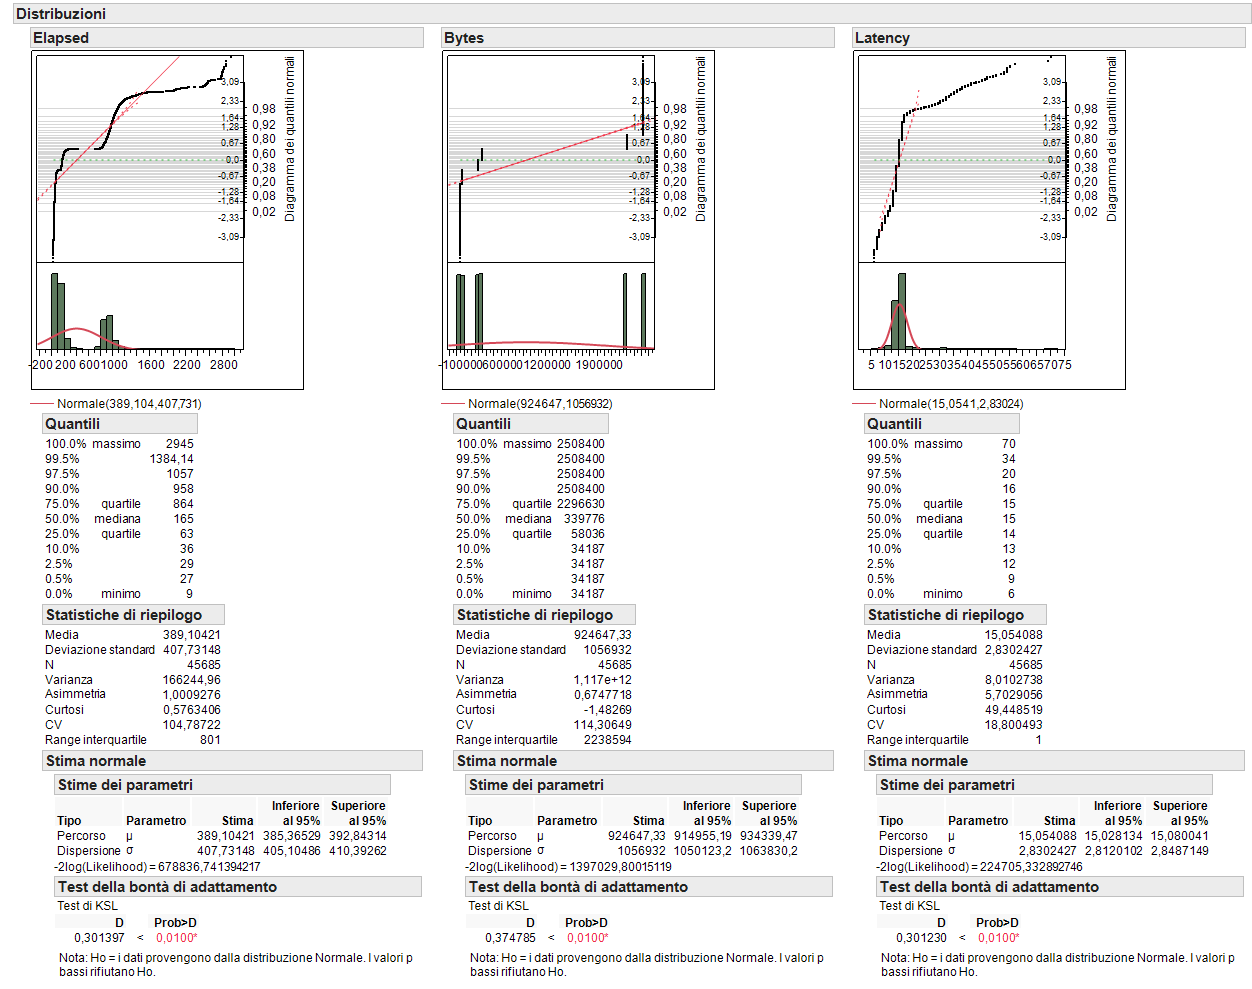
\includegraphics[width=1\linewidth, keepaspectratio]{distribuzioni_client}
  \caption{}
  \label{webserver_distribuzioni_parametri}
\end{figure}

Come si può osservare dal plot Q-Q e dal test di bontà di adattamento, le distribuzioni
non sono normali, di conseguenza, si scelgono \textit{mediana}, come indice di
tendenza centrale e \textit{SIQR}, come indice di dispersione.\\

\begin{center}
  \begin{tabular}{c|c|c|c|}
    & \textbf{Latency} & \textbf{Elapsed Time} & \textbf{Bytes} \\
    \hline
    \textbf{Mediana} & 15 & 165 & 339776 \\
    \hline
    \textbf{SIQR} & 1 & 801 & 2238594 \\
    \hline
  \end{tabular}
\end{center}

\subsubsection*{Correlazione Parametri}
Nella seguente fase vengono studiate possibili correlazioni presenti tra i tre
parametri considerati.\\
Per studiare la correlazione, non volendo fare assunzioni sulla natura delle
distribuzioni, è possibile svolgere il test non parametrico di \textbf{Kendall}.\\
Tale test assume come ipotesi nulla l'indipendenza dei fattori.\\
In particolare, si è interessati ad osservare eventuali correlazioni tra la Latency
e l'Elapsed Time, in \figurename~\ref{webserver_correlazione_elapsed_latency}.\\
\begin{figure}[!htbp]
  \centering
  \includegraphics[width=.7\linewidth, keepaspectratio]{correlazione_elapsed_latency}
  \caption{Test di Kendall tra i parametri Elapsed Time e Latency}
  \label{webserver_correlazione_elapsed_latency}
\end{figure}

In questo caso, il test di Kendall suggerisce che l'ipotesi di indipendenza è
rigettata, quindi esiste una forte dipendenza tra i parametri \textit{Latency} e
\textit{Elapsed Time}.

\subsection{Analisi Basso Livello (Server)}
Al fine di misurare il comportamento del server durante l'esperimento, si è
utilizzato il tool \textbf{collectl} simultaneamente all'avvio delle richieste
da parte del client.\\
Il comando lanciato nella bash \textit{Linux} è stato:\\
\begin{center}
  \textbf{collectl -oT -scdmn -P --sep ,}
\end{center}
in particolare:

\begin{itemize}
  \item \textbf{-oT}: aggiunge il timestamp;
  \item \textbf{-scdmn}:  permette di selezionare le periferica di cui si desidera
   monitorare i parametri di performance;
  \item \textbf{-P}: raggruppa i dati su una singola riga;
  \item \textbf{--sep ,}: utilizza la virgola come carattere separatore dei dati.
\end{itemize}

La \textbf{collectl} effettua una misurazione ogni secondo, in accordo al client
che monitora lo stato e le performance delle richieste effettuate.\\
Al fine di eliminare eventuali comportamenti anomali transitivi, l'esperimento è
stato condotto per 8 minuti, eliminando il primo e l'ultimo minuto.\\

Di seguito sono riportati i parametri considerati:
\begin{itemize}
  \item \textbf{CPU}:
  \begin{itemize}
    \item \textbf{\textit{Tot\%}}: percentuale di utilizzo della CPU;
    \item \textbf{\textit{Idle\%}}: percentuale di idle della CPU;
    \item \textbf{\textit{Interpt/sec}}: numero di interrupt al secondo;
    \item \textbf{\textit{Ctx/sec}}: numero di context switch al secondo.
  \end{itemize}
  \item \textbf{Disco}:
  \begin{itemize}
    \item \textbf{\textit{Reads}}: numero di letture al secondo;
    \item \textbf{\textit{RKBytes}}: KiloByte letti;
    \item \textbf{\textit{Writes}}: numero di scritture al secondo;
    \item \textbf{\textit{WKBytes}}: KiloByte scritti.
  \end{itemize}
  \item \textbf{RAM}:
  \begin{itemize}
    \item \textbf{\textit{Used}}: quantità di RAM fisica utilizzata;
    \item \textbf{\textit{Free}}: quantità di RAM fisica libera;
    \item \textbf{\textit{Buffered}}: quanti di RAM fisica utilizzata
    per bufferizzare file;
    \item \textbf{\textit{Cached}}: quantità di RAM fisica utilizzata come memoria cache;
    \item \textbf{\textit{Slab}}: quantità di memoria utilizzata dal kernel come cache per
    le strutture dati, per utilizzo proprio;
    \item \textbf{\textit{Map}}: quantità di memoria utilizzata
    per mappare dispositivi, file o librerie, tramite il comando mmap.
  \end{itemize}
  \item \textbf{Rete}
  \begin{itemize}
    \item \textbf{\textit{RxPkt}}: pacchetti ricevuti;
    \item \textbf{\textit{TxPkt}}: pacchetti trasmessi;
    \item \textbf{\textit{RxKB}}: KiloByte ricevuti;
    \item \textbf{\textit{TxKB}}: KiloByte inviati.
  \end{itemize}
\end{itemize}

Per la caratterizzazione del workload sono state utilizzate le tecniche di PCA e
Clustering.\\
\clearpage
\subsubsection{PCA}
Prima di applicare la PCA è stato analizzato l'andamento temporale dei parametri.\\
Quest'ultimo ha suggerito l'eliminazione dei parametri riguardanti il disco, dal
momento che, avendo eliminato il transitorio(primo ed ultimo minuto), il disco
non effettua alcuna operazione di lettura e/o scrittura in seguito a ulteriori
richieste http.\\
L'unico istante di tempo in cui il disco effettua una lettura è all'inizio
della sessione di test, in cui i dati relativi alle pagine sono caricati in RAM.\\
Nella seguente figura è riportato il primo minuto di test,
durante il quale si osserva un picco letture, con una notevole crescita della
memoria RAM utilizzata.\\

\begin{figure}[!htbp]
  \centering
  \includegraphics[width=\linewidth, keepaspectratio]{transitorio}
  \caption{Transitorio RAM/DISCO}
  \label{webserver_transitorio}
\end{figure}

\clearpage

Un'ulteriore analisi è stata fatta sul coefficiente di variazione,
per stabilire la presenza di parametri trascurabili, con \textit{CV} nullo.\\
Di seguito è riportato il coefficiente di variazione per ogni parametro.\\

\begin{figure}[!htbp]
  \centering
  \includegraphics[width=.4\linewidth, keepaspectratio]{cv}
  \caption{CV parametri CPU e RAM}
  \label{webserver_cv1}
\end{figure}
\clearpage
Sfortunatamente non è stato possibile eliminare alcun parametro, poiché non
presentano CV nullo, quindi è stata applicata direttamente la PCA all'intero
workload reale.\\
In \figurename~\ref{webserver_pca} è riportata il risultato ottenuto in JMP.\\

\begin{figure}[!htbp]
  \centering
  \includegraphics[width=1\linewidth, keepaspectratio]{pca}
  \caption{PCA}
  \label{webserver_pca}
\end{figure}

\begin{figure}[!htbp]
  \centering
  \includegraphics[width=1\linewidth, keepaspectratio]{autovalori}
  \caption{Autovalori PCA}
  \label{webserver_autovalori}
\end{figure}
\clearpage

\begin{figure}[!htbp]
  \centering
  \includegraphics[width=.8\linewidth, keepaspectratio]{scree_pca}
  \caption{Grafico Scree}
  \label{webserver_scree_pca}
\end{figure}

Osservando le Figure \ref{webserver_autovalori} e \ref{webserver_scree_pca} si è scelto di considerare
7 componenti principali conservando il 94,680\% di varianza.

\clearpage

\subsubsection{Clustering}
Dopo aver scelto il numero di componenti principali è stato applicato il clustering
per ridurre il numero di righe del workload reale.\\
In \figurename~\ref{webserver_clustering} è riportato il dendrogramma risultante dal
clustering gerarchico con la relativa curva di clustering, ottenuta in JMP.\\

\begin{figure}[!htbp]
  \centering
  \includegraphics[width=1\linewidth, keepaspectratio]{clustering}
  \caption{Clustering}
  \label{webserver_clustering}
\end{figure}
\clearpage

Osservando le figure \ref{webserver_clustering},
Infatti aggiungendo un ulteriore cluster, il guadagno ottenuto, in termini di varianza,
sarebbe stato trascurabile.\\

\begin{minipage}{\linewidth}
  \centering
  \begin{minipage}{0.48\linewidth}
    \begin{figure}[H]
      \includegraphics[width=0.9\linewidth]{gerarchia_cluster}
    \end{figure}
  \end{minipage}
  \begin{minipage}{0.48\linewidth}
    \begin{figure}[H]
      \includegraphics[width=.9\linewidth]{ccc}
    \end{figure}
  \end{minipage}
\end{minipage}
\captionof{figure}{Gerarchia di clustering e Criterio di Clusterizzazione Cubica}
\label{webserver_clustering}

\clearpage

\subsubsection{Caratterizzazione Cluster}
Per caratterizzare ogni cluster, ovvero per individuare quale stato del sistema
esso rappresentasse, sono state analizzate le figure \ref{webserver_autovettori}, \ref{webserver_graph}
e \ref{webserver_cluster_time}.\\
La figura \ref{webserver_autovettori} mostra gli autovettori delle 7 componenti principali,
dai quali è facile individuare i parametri del workload reale che maggiormente
incidono su ognuna di esse.\\
\begin{figure}[!htbp]
  \centering
  \includegraphics[width=.9\linewidth, keepaspectratio]{autovettori}
  \caption{Autovettori PCA}
  \label{webserver_autovettori}
\end{figure}

In particolare:

\begin{itemize}
  \item \textbf{\textit{Principale 1}}: influenzata maggiormente da parametri
  riguardanti la RAM.\\
  Nello specifico si nota che \textit{Used} e \textit{Free} si comportano in maniera duale;
  \item \textbf{\textit{Principale 2}}: influenzata maggiormente dai parametri
  di rete, \textit{Intrpt/sec} e \textit{Idle\%};
  \item \textbf{\textit{Principale 3}}: influenzata da \textit{Totl\%} e \textit{Idle\%};
  \item \textbf{\textit{Principale 4}}: influenzata da \textit{Map} e \textit{TxPktTot};
  \item \textbf{\textit{Principale 5}}: influenzata da \textit{Ctx/sec} e \textit{TxPktTot};
  \item \textbf{\textit{Principale 6}}: influenzata da \textit{Ctx/sec}, \textit{Map},
  \textit{RxPktTot}, \textit{TxPktTot} e \textit{RxKBTot};
  \item \textbf{\textit{Principale 7}}: influenzata da \textit{Buf} e \textit{Slab};
\end{itemize}

\clearpage

La figura \ref{webserver_graph} mostra quali sono le componenti principali che hanno contribuito
maggiormente alla creazione dei cluster.\\

\begin{figure}[!htbp]
  \centering
  \includegraphics[width=0.8\linewidth, keepaspectratio]{graph}
  \caption{}
  \label{webserver_graph}
\end{figure}
La figura \ref{webserver_cluster_time} mostra la composizione dei cluster rispetto al tempo.\\
\begin{figure}[!htbp]
  \centering
  \includegraphics[width=.8\linewidth, keepaspectratio]{cluster_time}
  \caption{}
  \label{webserver_cluster_time}
\end{figure}

\clearpage

Di seguito è riportata la caratterizzazione dei singoli cluster ed una loro
rappresentazione grafica 3D, in funzione di tre componenti principali.\\
In questi grafici i campioni plottati hanno una sfumatura dal blu al rosso, in
funzione del tempo, in cui il blu rappresenta il primo minuto del test ed il
rosso l'ultimo.\\

\begin{itemize}

  \begin{figure}[!htbp]
    \centering
    \includegraphics[width=.45\linewidth, keepaspectratio]{cluster1}
    \caption{Grafico 3D del Cluster 1}
    \label{webserver_cluster1}
  \end{figure}

  \item \textbf{Cluster 1}: influenzato maggiormente da valori negativi della
  1 e 2 componente principale e positivi della 6.\\
  In particolare, osservando la figura \ref{webserver_cluster_time} e \ref{webserver_cluster1}, i campioni contenuti
  in questo cluster appartengono alla prima metà dell'esperimento.\\
  Analizzando più approfonditamente la cause della creazione di tale cluster si
  identifica quale stato del sistema esso rappresenta.\\
  A causa di valori negativi della prima componente principale esso
  rappresenta uno stato del sistema con bassa occupazione della memoria RAM,
  in quanto il valore della parametro \textit{Free} nei campioni del cluster 1,
  essendo negativo in corrispondenza della principale 1 in figura \ref{webserver_autovettori},
  fornisce sicuramente un impatto maggiore rispetto agli altri parametri.\\
  Inoltre si può affermare che a causa della seconda componente principale negativa
  l'attività di rete è bassa, in quanto nella figura \ref{webserver_autovettori} si osserva
  che i parametri di rete influenzano positivamente la principale due, di conseguenza
  per assumere valori negativi, i parametri di rete devono assumere valori bassi.

  \clearpage

  \begin{figure}[!htbp]
    \centering
    \includegraphics[width=.45\linewidth, keepaspectratio]{cluster2}
    \caption{Cluster 2}
    \label{webserver_cluster2}
  \end{figure}

  \item \textbf{Cluster 2}: influenzato maggiormente da valori negativi della
  1 e positivi della 2 e 4 componente principale.\\
  In particolare, osservando la figura \ref{webserver_cluster_time} e \ref{webserver_cluster1}, i campioni contenuti
  in questo cluster appartengono alla prima metà dell'esperimento.\\
  Analizzando più approfonditamente la cause della creazione di tale cluster si
  identifica quale stato del sistema esso rappresenta.\\
  In particolare il cluster rappresenta uno stato del sistema in cui la quantità di RAM occupata
  è bassa, comportamento verificato nel primo cluster, ma in maniera opposta,
  essendo positiva la principale due e presentando un'attività di rete più intensa.

  \clearpage

  \begin{figure}[!htbp]
    \centering
    \includegraphics[width=0.45\linewidth, keepaspectratio]{cluster3}
    \caption{Cluster 3}
    \label{webserver_cluster3}
  \end{figure}

  \item \textbf{Cluster 3}: influenzato maggiormente da valori negativi della
  1 e 7 principale, e positivi della 5.\\
  In particolare, osservando la figura \ref{webserver_cluster_time} e \ref{webserver_cluster1}, i campioni contenuti
  in questo cluster appartengono ad un intervallo temporale centrale dell'esperimento.\\
  Analizzando più approfonditamente la cause della creazione di tale cluster si
  identifica quale stato del sistema esso rappresenta.\\
  In particolare il cluster rappresenta uno stato in cui la quantità di RAM occupata
  è bassa, comportamento verificato nel primo cluster, con attività di rete in trasmissione
  bassa e aumento delle memoria RAM dedicata al buffering dei file.

  \clearpage

  \begin{figure}[!htbp]
    \centering
    \includegraphics[width=.45\linewidth, keepaspectratio]{cluster4}
    \caption{Cluster 4}
    \label{webserver_cluster4}
  \end{figure}

  \item \textbf{Cluster 4}: presenta valori delle componenti principali per cui non
  è possibile una corretta caratterizzazione.\\
  Per poter essere ugualmente analizzato, il cluster è stato suddiviso in due
  sotto-cluster, utilizzando la cronologia di clusterizzazione mostrata in
  precedenza.\\
  In figura \ref{webserver_cluster_4_diviso} è riportata l'incidenza delle componenti
  principali sui due sotto-cluster.\\

  \begin{figure}[!htbp]
    \centering
    \includegraphics[width=.6\linewidth, keepaspectratio]{cluster_4_diviso}
    \caption{}
    \label{webserver_cluster_4_diviso}
  \end{figure}

  Dalla figura \ref{webserver_cluster_4_diviso} si possono caratterizzare i cluster 4.1 e 4.2.\\
  Il cluster 4.1 risulta influenzato  negativamente dalle principali 1 e 4
  e positivamente dalla principale 2, quindi c'è un alta attività di rete
  e una bassa quantità di memoria RAM occupata.\\
  Il cluster 4.2 risulta influenzato negativamente dalle principali 6 e 4,
  e positivamente dalla principale 1.\\
  Dunque si evince un'alta attività di rete ed un'elevata occupazione di memoria
  RAM.\\

  \begin{figure}[!htbp]
    \centering
    \includegraphics[width=.45\linewidth, keepaspectratio]{cluster41}
    \caption{Cluster 4.1}
    \label{webserver_cluster41}
  \end{figure}

  \begin{figure}[!htbp]
    \centering
    \includegraphics[width=.45\linewidth, keepaspectratio]{cluster42}
    \caption{Cluster 4.2}
    \label{webserver_cluster42}
  \end{figure}

  \clearpage

  \begin{figure}[!htbp]
    \centering
    \includegraphics[width=.4\linewidth, keepaspectratio]{cluster5}
    \caption{Cluster 5}
    \label{webserver_cluster5}
  \end{figure}

  \item \textbf{Cluster 5}: tale cluster è formato da un solo campione, essendo
  esso un outlier, necessita di essere analizzato per capire se è possibile eliminarlo.\\
  La creazione di tale cluster è attribuita maggiormente alla principale
  2, condizionata a sua volta dai parametri \textbf{RxPktTot} e \textbf{RxKBTot}.\\
  Analizzando il grafico in figura \ref{webserver_cluster5_temp_analisi}, il quale riporta
  l'andamento temporale di \textbf{RxKBTot}, si osserva che in corrispondenza del
  cluster 5 c'è un picco negativo il quale può essere attribuito ad una riduzione
  della velocità di trasmissione del client.\\
  Quindi è stato deciso di non considerare tale cluster nella fase finale di
  generazione del workload sintetico.\\

  \begin{figure}[!htbp]
    \centering
    \includegraphics[width=.5\linewidth, keepaspectratio]{cluster5_temp_analisi}
    \caption{Andamento temporale di RxPktTot}
    \label{webserver_cluster5_temp_analisi}
  \end{figure}

  \clearpage

  \begin{figure}[!htbp]
    \centering
    \includegraphics[width=0.45\linewidth, keepaspectratio]{cluster6}
    \caption{Cluster 6}
    \label{webserver_cluster6}
  \end{figure}

  \item \textbf{Cluster 6}: la formazione di tale cluster è attribuita alle
  componenti principali 2,3 e 5, le quali sono state influenzate maggiormente
  da \textit{RxPktTot}, \textit{Tot\%}, \textit{TxPktTot} e \textit{Ctx/s}.\\
  Analizzando la figura \ref{webserver_analisi_temp_cluster_6}, la quale riporta l'andamento
  temporale dei parametri sopra descritti, si nota che tali campioni sono consecutivi
  e individuano un picco di \textit{Ctx/s}, il quale può essere attributo all'esecuzione
  di altri processi presenti nel server.\\
  A tal proposito si può ritenere irrilevante tale cluster ai fini della
  caratterizzazione del workload sintetico.\\

  \begin{figure}[!htbp]
    \centering
    \includegraphics[width=0.6\linewidth, keepaspectratio]{analisi_temp_cluster_6}
    \caption{Analisi temporale \textit{RxPktTot}, \textit{Tot\%}, \textit{TxPktTot} e \textit{Ctx/s}}
    \label{webserver_analisi_temp_cluster_6}
  \end{figure}

  \clearpage

  \begin{figure}[!htbp]
    \centering
    \includegraphics[width=.45\linewidth, keepaspectratio]{cluster7}
    \caption{Cluster 7}
    \label{webserver_cluster7}
  \end{figure}

  \item \textbf{Cluster 7}: la formazione di tale cluster è attribuibile maggiormente
  alla 3 componente principale, la quale è stata influenza dal parametro \textit{Tot\%}.\\
  Analizzando il comportamento temporale di tale parametro, in figura \ref{webserver_analisi_temp_cluster_7},
  si osserva che tale cluster contiene picchi di utilizzo della CPU, ad ogni
  occorrenza del primo secondo di ogni minuto di test.\\
  \'E stato monitorato il sistema server anche in assenza di esecuzione del workload,
  e tale fenomeno ha continuato a manifestarsi, dimostrandosi inerente al
  comportamento del sistema operativo.\\
  Per questo motivo questo cluster non è stato considerato ai fini della
  caratterizzazione del workload sintetico.\\

  \begin{figure}[!htbp]
    \centering
    \includegraphics[width=0.6\linewidth, keepaspectratio]{analisi_temp_cluster_7}
    \caption{Analisi temporale \textit{Tot\%}}
    \label{webserver_analisi_temp_cluster_7}
  \end{figure}

  \clearpage

  \begin{figure}[!htbp]
    \centering
    \includegraphics[width=.45\linewidth, keepaspectratio]{cluster8}
    \caption{Cluster 8}
    \label{webserver_cluster8}
  \end{figure}

  \item \textbf{Cluster 8}: rappresenta la parte finale dell'esperimento.\\
  Lo stato del sistema che esso rappresenta è dato da un'elevata occupazione
  di RAM ed una bassa attività di rete, risultando essere il duale del \textit{cluster 1}.\\

\end{itemize}
\clearpage
Scegliendo come punti rappresentanti ogni cluster il loro centroide, il Workload
Sintetico ottenuto è il seguente.
\begin{figure}[!htbp]
  \centering
  \includegraphics[width=1\linewidth, keepaspectratio]{centroidi}
  \caption{Workload Sintetico}
  \label{webserver_centroidi}
\end{figure}

La percentuale di devianza persa approssimando il workload reale con quello
sintetico è il \textbf{33,27\%}.

\begin{minipage}{\linewidth}
  \centering
  \begin{minipage}{0.48\linewidth}
    \begin{figure}[H]
      \includegraphics[width=0.9\linewidth]{devianza}
    \end{figure}
  \end{minipage}
  \begin{minipage}{0.48\linewidth}
    \begin{figure}[H]
      \includegraphics[width=.9\linewidth]{significativita_workload}
    \end{figure}
  \end{minipage}
\end{minipage}

\clearpage

\section{Capacity Test}
Questa sezione è dedicata allo studio della capacità di carico del sistema.\\
Il capacity test è attuato sulla base del workload caratterizzato in precedenza,
in funzione della tipologia di richieste effettuate al server(pagine di
piccola, media e grande dimensione).\\
I parametri di interesse nel capacity test sono le \textit{Richieste al minuto(Req/min)},
il \textit{Throughput} e l'\textit{Elapsed Time}.\\
Il test procede incrementando le Req/min ed osservando i 2 parametri di risposta
del sistema.\\
Plottando i risultati ottenuti è possibile individuare due punti di funzionamento
del sistema, noti come:
\begin{itemize}
  \item \textbf{Knee Capacity} - punto di funzionamento in cui il sistema ha un
  buon throughput e dei tempi di risposta bassi;
  \item \textbf{Usable Capacity} - punto di funzionamento limite in cui il sistema
  ha un ottimo throughput, ma oltre il quale c'è un degrado notevole nelle prestazioni.
\end{itemize}

Per il test effettuato con il tool JMeter, è stato scelto di di simulare 50 Threads
attivi.\\

\subsection{Test pagine HTML piccole}
In questo caso sono state utilizzate esclusivamente le richieste HTTP per le pagine
\textit{small\_text} e \textit{small\_image}.\\
In \figurename~\ref{webserver_small_page_summary_report} sono presenti gli esiti del
Summary Report di JMeter.\\

\begin{figure}[!htbp]
  \centering
  \includegraphics[width=.4\linewidth, keepaspectratio]{capacitytest_small}
  \caption{Test pagine HTML piccole}
  \label{webserver_small_page_summary_report}
\end{figure}

Utilizzando il costruttore di Grafici di \textit{JMP} sono stati analizzati i plot
di Throughput ed Elapsed Time, e definiti i punti di \textit{Knee Capacity} e
\textit{Usable Capacity}.\\

\begin{figure}[!htbp]
  \centering
  \includegraphics[width=\linewidth, keepaspectratio]{usable_knee_small}
  \caption{Capacity: Knee (15000 Req/min) / Usable (60000 Req/min)}
\end{figure}

\subsection{Test pagine HTML medie}
In questo caso sono state utilizzate esclusivamente le richieste HTTP per le pagine
\textit{medium\_text} e \textit{medium\_image}.\\
In \figurename~\ref{webserver_medium_page_summary_report} sono presenti gli esiti del
Summary Report di JMeter.\\

\begin{figure}[!htbp]
  \centering
  \includegraphics[width=.4\linewidth, keepaspectratio]{capacitytest_medium}
  \caption{Test pagine HTML medie}
  \label{webserver_medium_page_summary_report}
\end{figure}

Utilizzando il costruttore di Grafici di \textit{JMP} sono stati analizzati i plot
di Throughput ed Elapsed Time, e definiti i punti di \textit{Knee Capacity} e
\textit{Usable Capacity}.\\

\begin{figure}[!htbp]
  \centering
  \includegraphics[width=\linewidth, keepaspectratio]{usable_knee_medium}
  \caption{Capacity: Knee (2000 Req/min) / Usable (30000 Req/min)}
\end{figure}

\clearpage

\subsection{Test pagine HTML grandi}
In questo caso sono state utilizzate esclusivamente le richieste HTTP per le pagine
\textit{big\_text} e \textit{big\_image}.\\
In \figurename~\ref{webserver_big_page_summary_report} sono presenti gli esiti del
Summary Report di JMeter.\\

\begin{figure}[!htbp]
  \centering
  \includegraphics[width=.4\linewidth, keepaspectratio]{capacitytest_big}
  \caption{Test pagine HTML grandi}
  \label{webserver_big_page_summary_report}
\end{figure}

Utilizzando il costruttore di Grafici di \textit{JMP} sono stati analizzati i plot
di Throughput ed Elapsed Time, e definiti i punti di \textit{Knee Capacity} e
\textit{Usable Capacity}.\\

\clearpage

\begin{figure}[!htbp]
  \centering
  \includegraphics[width=\linewidth, keepaspectratio]{usable_knee_big}
  \caption{Capacity: Knee (1500 Req/min) / Usable (3000 Req/min)}
\end{figure}

\subsection{Test Random}
Finora sono state studiate le capacità di carico del sistema in presenza delle
tre differenti tipologie di pagine HTML disponibili.\\
Dai test effettuati è possibile ricavare il caso medio e il caso peggiore per
ognuno dei punti di funzionamento considerati:
\begin{itemize}
  \item Caso Medio:
  \begin{itemize}
    \item \textbf{Knee Capacity} - 6167
    \item \textbf{Usable Capacity} - 31000
  \end{itemize}
  \item Caso Peggiore:
  \begin{itemize}
    \item \textbf{Knee Capacity} - 1500
    \item \textbf{Usable Capacity} - 3000
  \end{itemize}
\end{itemize}

Come era possibile aspettarsi, il caso peggiore corrisponde esattamente all'uso
delle pagine HTML grandi.\\

Per verificare il reale comportamento del sistema, è stato effettuato un ulteriore
capacity test per definire i punti di funzionamento nel caso di un Random Controller
che genera, in maniera uniforme, richieste HTTP relative a tutte le tipologie di
pagine.\\

In \figurename~\ref{webserver_random_page_summary_report} sono presenti gli esiti del
Summary Report di JMeter.\\

\begin{figure}[!htbp]
  \centering
  \includegraphics[width=.4\linewidth, keepaspectratio]{capacitytest_random}
  \caption{Test pagine random}
  \label{webserver_random_page_summary_report}
\end{figure}

Utilizzando il costruttore di Grafici di \textit{JMP} sono stati analizzati i plot
di Throughput ed Elapsed Time, e definiti i punti di \textit{Knee Capacity} e
\textit{Usable Capacity}.\\

\begin{figure}[!htbp]
  \centering
  \includegraphics[width=\linewidth, keepaspectratio]{usable_knee_random}
  \caption{Capacity: Knee (2000 Req/min) / Usable (8000 Req/min)}
\end{figure}

\clearpage

\section{Design of Experiments}
Scopo ultimo del DOE è riuscire ad ottenere un design tale da
massimizzare le informazioni ottenute, minimizzando il numero di esperimenti
necessari.\\
Una corretta analisi degli esperimenti aiuta anche a separare gli effetti dei
vari fattori che potrebbero influenzare le prestazioni, determinando se un fattore
è \textit{significativo} oppure se le differenze osservate dipendono semplicemente
da variazioni casuali dovute ad errori di misura e/o parametri non controllabili.\\
Inoltre, il design of experiments è fondamentale anche per ridurre il numero di
esperimenti, quindi il costo, necessari al testing del sistema.\\
Per fare ciò è stata utilizzata la funzionalità \textit{Piano Fattoriale Completo},
resa disponibile dal tool JMP e configurata come in figura \ref{webserver_piano_fattoriale_completo}.\\

\begin{figure}[!htbp]
  \centering
  \includegraphics[width=.9\linewidth, keepaspectratio]{doe_setup}
  \caption{Piano Fattoriale Completo}
  \label{webserver_piano_fattoriale_completo}
\end{figure}

\clearpage

Nel piano fattoriale completo sono stati utilizzati come risposta di interesse,
l'\textit{Average Response Time}(tempo medio di risposta), come fattori il
\textit{Page Size}(categorico a 3 livelli) ed il \textit{Request Rate}(categorico
 a 4 livelli).\\
Il request rate è stato calcolato in funzione della dimensione della pagina,
ed è in particolare definito su 4 livelli:
\begin{itemize}
  \item \textbf{Low} - 20\% della usable capacity
  \item \textbf{Low-Mid} - 40\% della usable capacity
  \item \textbf{High-Mid} - 60\% della usable capacity
  \item \textbf{High} - 80\% della usable capacity
\end{itemize}

In figura \ref{webserver_fattori} sono riportate le capacità usate per ogni dimensione di
pagina e per ogni categoria di carico.\\

\begin{figure}[!htbp]
  \centering
  \includegraphics[width=.7\linewidth, keepaspectratio]{fattori}
  \caption{Req/min al variare del carico e della tipologia di pagina}
  \label{webserver_fattori}
\end{figure}

\clearpage

\subsection{Modello}
In seguito ai 120 esperimenti effettuati è possibile stimare il modello ottenuto.\\
Fare ciò in JMP è molto semplice grazie alla funzionalità \textit{Stima Modello},
riportata in figura \ref{webserver_stima_modello}

\begin{figure}[!htbp]
  \centering
  \includegraphics[width=.6\linewidth, keepaspectratio]{stima_modello}
  \caption{Stima del modello ottenuto}
  \label{webserver_stima_modello}
\end{figure}

Osservando il \textbf{coefficiente di determinazione}($R^{2}$) è possibile
immediatamente affermare che il modello effettua un ottimo fitting dei dati.\\
Infatti il modello spiega circa il 99.8\% della devianza totale.\\
Nell'analisi della varianza riportata in figura \ref{webserver_stima_modello} è possibile anche
osservare che il modello ottenuto è significativo con un livello di confidenza
del 95\%, essendo il test di Fisher rigettato con un $p-value<0.001$.\\

\subsection{Importanza e Significatività Statistica dei fattori}
Importanza e Significatività sono 2 concetti utili e distinti per l'analisi dei
fattori ed entrambi appartengono alla categoria di tecniche
\textbf{ANOVA}(ANalysis Of VAriance).\\
Un fattore è tanto più \textit{importante} quanto ha un rapporto $\frac{SSA}{SST}$
elevato.\\
Un fattore importante non necessariamente è significativo, infatti nella significatività
entrano in gioco anche i \textbf{gradi di libertà}.\\
La significatività di un fattore può anche essere vista come la robustezza del
modello rispetto all'errore e può essere studiata utilizzando un test sulla
varianza.\\

\subsubsection{Importanza}
In figura \ref{webserver_importanza_fattori} sono riportati i valori di importanza dei due
fattori in studio.

\begin{figure}[!htbp]
  \centering
  \includegraphics[width=.9\linewidth, keepaspectratio]{importanza_fattori}
  \caption{Importanza dei Fattori}
  \label{webserver_importanza_fattori}
\end{figure}

Come si evince dalla tabella, il fattore più importante è il \textbf{Page Size},
essendo quello che incide maggiormente sull'elapsed time.\\
Inoltre l'errore risulta essere molto basso, a verifica di quanto affermato dal
coefficiente di determinazione.\\

\clearpage

\subsubsection{Significatività Statistica}
L'analisi della significatività statistica dei fattori basata su ANOVA richiede
che due forti assunzioni siano soddisfatte: \textbf{Normalità} ed
\textbf{Omoschedasticità}.\\
Nel caso in cui una delle due, o entrambe le assunzioni, non siano soddisfatte, è
possibile fare ausilio di ulteriori tecniche e test non parametrici per analizzare
la significatività dei fattori.\\

\subsubsection*{Normalità}
La normalità è studiata sui residui relativi al modello, ottenibili semplicemente
in JMP dalla scheda di \textit{Stima del Modello}.\\
In figura \ref{webserver_normalita} è riportata la distribuzione dei residui ed il test
di \textit{Shapiro-Wilk} per la normalità su un campione di $N<2000$ esperimenti.\\
Il test suggerisce un $p-value<0.001$, quindi l'ipotesi di normalità è rigettata
con il 95\% di confidenza.\\

\begin{figure}[!htbp]
  \centering
  \includegraphics[width=\linewidth, keepaspectratio]{normalita}
  \caption{Normalità dei residui del modello stimato}
  \label{webserver_normalita}
\end{figure}

\clearpage

\subsubsection*{Omoschedasticità}
L'omoschedasticità è studiata sui residui del modello un fattore per volta,
essendo essa la proprietà di costanza della varianza, al variare dei livelli di
ogni singolo fattore.\\
Per fare ciò in JMP, non è studiata la distribuzione dei residui,
ma è effettuata una \textit{Stima Y rispetto X}, per ciascun fattore.\\
In figura \ref{webserver_omoschedasticita} è possibile osservare che il test di \textbf{Levene},
scelto per analizzare l'omoschedasticità dei residui rispetto ai singoli fattori,
dà risultato negativo, rigettando l'ipotesi nulla in entrambi i casi.\\
\'E stato scelto in particolare il test di Levene e non altri per la sua
robustezza a situazioni di non normalità dei dati.\\

\begin{figure}[!htbp]
  \centering
  \includegraphics[width=\linewidth, keepaspectratio]{omoschedasticita}
  \caption{Omoschedasticità dei residui rispetto ai fattori}
  \label{webserver_omoschedasticita}
\end{figure}

\clearpage

Avendo stabilito che il modello stimato non soddisfa le assunzioni di normalità e
omoschedasticità, non è possibile utilizzare l'ANOVA classico con il Fisher-Test
per studiare la significatività dei fattori, bensì il \textit{Kruskal-Wallis Test}.\\

In figura \ref{webserver_kruskal_wallis_significativita} si osservano gli esiti del test
di significatività effettuato su entrambi i fattori.\\
Come da attesa, il fattore \textit{Page Size} è molto significativo,
essendo l'ipotesi nulla pienamente rigettata.\\
Il fattore \textit{Request Rate}, viceversa, è meno significativo
del Page Size, non potendo essere rigettata l'ipotesi nulla con il 95\% di
confidenza, ma solo con il 90\% circa.\\

\begin{figure}[!htbp]
  \centering
  \includegraphics[width=\linewidth, keepaspectratio]{kruskal_wallis_significativita}
  \caption{Kruskal-Wallis Test per la significatività dei fattori}
  \label{webserver_kruskal_wallis_significativita}
\end{figure}

	% !TEX root = ./main.tex
% !TEX encoding = UTF-8 Unicode
% !TEX program = pdflatex
% !TeX spellcheck = it_IT

\graphicspath{{Immagini/},{Immagini/android_aging/}}

\chapter{Software Aging on Android 7}

\section{Traccia}
Verificare se \textbf{Android} è soggetto ad \textbf{\textit{aging}}.\\

\section{System Under Test}
Il dispositivo utilizzato è un \textbf{Huawei P9 Lite}, con le seguenti caratteristiche:

\begin{itemize}
  \item \textbf{Chipset: }Kirin 650 (4 x 2,0GHz + 4 x 1,7GHZ) 64 bit
  \item \textbf{Memoria: } 3GB RAM, 16GB EMMC Flash ROM
  \item \textbf{Sistema Operativo: }Android 7.0
\end{itemize}

\section{Experimental Plan}

Per verificare il fenomeno dell'\textbf{Aging} sarà analizzato il \textbf{Lunch Time(LT)},
misura del tempo tra il click sull'icona dell'applicazione e l'avvio della stessa,
in quanto il fenomeno dell'aging, dal punto di vista dell'utente, è percepito
come una bassa reattività del dispositivo.\\
Gli indicatori di aging del sistema sono invece parametri che riguardano la \textit{memoria},
la \textit{Garbage Collection} ed il \textit{Task-Level}.\\

\section{Experimental Setup}

Gli esperimenti sono stati eseguiti su uno smartphone \textit{Huawei P9 Lite}, descritto
in precedenza, utilizzando il tool \textit{\textbf{ADB(Android Debug Bridge)}}.\\
La generazione del workload è stata effettuata tramite il tool
\textit{\textbf{Monkey WL generator}}, mentre la raccolta dei dati tramite le
utility \textit{\textbf{dumpsys}} e \textit{\textbf{logcat}}.\\
In figura \ref{and_setup} è riportato lo schema di connessione con il quale sono stati
eseguiti gli esperimenti.\\
La connessione tra PC e smartphone è stata realizzata tramite WiFi, quindi è
stato generato il workload tramite \textit{\textbf{Monkey WL generator}}, inviato
tramite WiFi al dispositivo mobile ed infine i dati sono stati raccolti
utilizzando \textit{\textbf{dumpsys}} e \textit{\textbf{logcat}}.\\

\begin{figure}[!htbp]
  \centering
  \includegraphics[width=\linewidth, keepaspectratio]{setup}
  \caption{Setup esperimenti}
  \label{and_setup}
\end{figure}

In totale sono stati eseguiti due test:
\begin{itemize}
  \item \textbf{Workload Fisso};
  \item \textbf{Workload Variabile}.
\end{itemize}

Il primo esperimento è un test di durata di 6 ore, cui obiettivo è stressare il
dispositivo effettuando un'operazione ogni 100ms.\\
Il secondo esperimento è un test che punta ad osservare il comportamento del dispositivo
in un utilizzo normale, con il tipico carico di un utente medio, effettuando
delle operazioni ad intervallo di tempo variabile(500ms, 1500ms e 2500ms).\\
Questo secondo test a workload variabile, sovraccaricando meno il sistema, ha una
durata complessiva di 12 ore.\\
In generale, in entrambi i test, il workload genera i seguenti movimenti
\begin{itemize}
  \item \textbf{Touch, Motion and Trackballs (33\%)};
  \item \textbf{(minor and major) Navigation (33\%)};
  \item \textbf{AppSwitch (34\%)}.
\end{itemize}
Le applicazioni utilizzate per gli esperimenti, riportate nella tabella in figura
\ref{and_applicazioni}, sono state ottenute lanciando il comando
\textit{adb shell pm list packages}.\\

\begin{figure}[!htbp]
  \centering
  \includegraphics[width=\linewidth, keepaspectratio]{applicazioni}
  \caption{Applicazioni Workload}
  \label{and_applicazioni}
\end{figure}

L'esecuzione degli esperimenti è stata effettuata lanciando lo script bash
\textit{\textbf{runtest.sh}} il quale richiama i seguenti script:
  \begin{itemize}
    \item \textit{\textbf{logcat\_art.sh}}: raccoglie i dati relativi al \textit{Garbage Collector};
    \item \textit{\textbf{dumpTask.sh}}: raccoglie i dati relativi ai task;
    \item \textit{\textbf{dumpOnlyMeminfo.sh}}: raccoglie i dati relativi alla memoria;
    \item \textit{\textbf{loagcat\_displayed.sh}}: raccoglie i dati relativi al LT;
    \item \textit{\textbf{kill\_after\_time.sh}}: permette di definire il tempo di
    sperimentazione ed esegue il reboot in modalità recovery del dispositivo;
    \item \textit{\textbf{LaunchTimeMeasurement.sh}}: esegue lo stress test del dispositivo;
    \item \textit{\textbf{WorkloadFixed.sh o WorkloadVariable.sh}}: il primo definisce le applicazioni del
    workload fisso, il secondo definisce l'esecuzione del workload variabile, richiamando
    a sua volta ulteriori 3 script, nei quali sono definite le applicazioni da lanciare.
  \end{itemize}

\section{Data Analysis}

L'esecuzione dello script \textbf{\textit{runtest.sh}} genera diversi file di log
tra cui \textit{\textbf{Displyed.txt}} e \textit{\textbf{meminfo.txt}}, i quali
contengono rispettivamente i dati relativi ai tempi di lancio delle activity ed
i dati relativi all'utilizzo della memoria.\\
L'analisi relativa ai tempi di lancio è effettuata tramite lo script \textbf{\textit{generate\_Time\_data.sh}},
il quale estrae una serie temporale per ogni activity, sulla quale effettua,
tramite un script R, il \textbf{\textit{Mann Kendall test}} con intervallo
di confidenza al 90\%.\\
Il \textbf{\textit{Mann Kendall test}} è un test che mira a verificare l'esistenza
di un trend nei dati.\\
Valori bassi del p-value rifiutano $H_0$, ovvero l'esistenza del trend.\\
Inoltre lo script genera i plot per ogni activity.\\
L'analisi relativa alla memoria è effettuata tramite i seguenti script:
\begin{itemize}
  \item \textit{\textbf{generate\_Meminfo\_data.sh}}:
  \item \textit{\textbf{generate\_Global\_Meminfo\_data.sh}}: genera le statistiche
  globali per i parametri di memoria RAM e i relativi plot temporali;
  \item \textit{\textbf{generate\_Meminfo\_data\_Slopes.sh}}: esegue il \textbf{\textit{Mann Kendal test}}
  per ogni task attivo sul dispositivo;
\end{itemize}

\clearpage

\subsection{Launch Time Analysis(Worklaod Fixed)}
Dopo aver analizzato i valori di \textit{slope}(pendenza della retta) e
\textit{p-value}(relativo al Mann Kendall test), si osserva, in figura \ref{and_analisi_trend_lt_activity_1},
che alcune activity presentano un trend positivo, anche se la crescita
del loro LT non è significativa poiché il valore slope non è sufficientemente
alto.\\
Quanto affermato è validato dai i plot ottenuti eseguendo lo script
\textit{\textbf{generate\_Meminfo\_data.sh}}.

\begin{figure}[!htbp]
  \centering
  \includegraphics[width=\linewidth, keepaspectratio]{analisi_trend_lt_activity_1}
  \caption{Trend Activity Workload Fixed}
  \label{and_analisi_trend_lt_activity_1}
\end{figure}

\clearpage

\subsection{Launch Time Analysis(Worklaod Variable)}
Dopo aver analizzato i valori di \textit{slope}(pendenza della retta) e
\textit{p-value}(relativo al Mann Kendall test), si osserva, in figura \ref{and_analisi_trend_lt_activity_2},
che alcune activity presentano un trend positivo, anche se la crescita
del loro LT non è significativa poiché il valore slope non è sufficientemente
alto.\\
Quanto affermato è validato dai i plot ottenuti eseguendo lo script
\textit{\textbf{generate\_Meminfo\_data.sh}}.

\begin{figure}[!htbp]
  \centering
  \includegraphics[width=\linewidth, keepaspectratio]{analisi_trend_lt_activity_2}
  \caption{Trend Activity Workload Fixed}
  \label{and_analisi_trend_lt_activity_2}
\end{figure}

\clearpage

\subsection{Memory Analysis(Worklaod Fixed)}

Nell'analisi a basso livello verrà considerato il parametro PSS(Proportional Set Size)
dei processi \textit{system}, \textit{systemui}, \textit{mediaserver} e
\textit{surfaceflinger}, per i quali sarà verificata l'esistenza di un trend.\\

\begin{figure}[!htbp]
  \centering
  \includegraphics[width=.3\linewidth, keepaspectratio]{pvalue_memoria_1}
  \caption{System}
  \label{and_pvalue_memoria_1}
\end{figure}

Nella tabella in figura \ref{and_pvalue_memoria_1} sono riportati i p-value associati
al \textit{Mann Kendall test}.\\
Quest'ultimo suggerisce che può essere rigettata l'ipotesi nulla, dimostrando
che in tutte le serie temporali esiste un trend.\\
In particolare, osservando le immagini in figura \ref{and_minipage_trends}, si verifica che effettivamente
tutti i processi presentano un trend, in particolare \textit{mediaserver},
il quale presenta un trend negativo.\\
Il trend più significativo è verificato nei processi \textit{system} e \textit{systemui}.

\begin{minipage}{\linewidth}
  \centering
  \begin{minipage}{0.49\linewidth}
    \begin{figure}[H]
      \includegraphics[width=\linewidth]{system_1}
    \end{figure}
  \end{minipage}
  \begin{minipage}{0.49\linewidth}
    \begin{figure}[H]
      \includegraphics[width=\linewidth]{systemui_1}
    \end{figure}
  \end{minipage}
  \begin{minipage}{0.49\linewidth}
    \begin{figure}[H]
      \includegraphics[width=\linewidth]{mediaserver_1}
    \end{figure}
  \end{minipage}
  \begin{minipage}{0.49\linewidth}
    \begin{figure}[H]
      \includegraphics[width=\linewidth]{surfaceflinger_1}
    \end{figure}
  \end{minipage}
\end{minipage}
\captionof{figure}{Trends in system, systemui, mediaserver, surfaceflinger}
\label{and_minipage_trends}

\clearpage
\subsection{Memory Analysis(Worklaod Variable)}

Nell'analisi a basso livello verrà considerato il parametro PSS dei processi \textit{system},
\textit{systemui}, \textit{mediaserver} e \textit{surfaceflinger}, dei quali
sarà verificata l'esistenza di un trend.\\

\begin{figure}[!htbp]
  \centering
  \includegraphics[width=.3\linewidth, keepaspectratio]{pvalue_memoria_1}
  \caption{System}
  \label{and_pvalue_memoria_1}
\end{figure}

Nella tabella in figura \ref{and_pvalue_memoria_1} sono riportati i p-value associati
al \textit{Mann Kendall test}.\\
Quest'ultimo suggerisce che può essere rigettata l'ipotesi nulla, dimostrando
che in tutte le serie temporali esiste un trend.\\
In particolare, osservando le immagini in figura \ref{and_minipage_trends2}, si verifica che effettivamente
tutti i processi presentano un trend, in particolare \textit{mediaserver},
il quale presenta un trend negativo.\\
Il trend più significativo è verificato nei processi \textit{system} e \textit{systemui}.

\begin{minipage}{\linewidth}
  \centering
  \begin{minipage}{0.49\linewidth}
    \begin{figure}[H]
      \includegraphics[width=\linewidth]{system_2}
    \end{figure}
  \end{minipage}
  \begin{minipage}{0.49\linewidth}
    \begin{figure}[H]
      \includegraphics[width=\linewidth]{systemui_2}
    \end{figure}
  \end{minipage}
  \begin{minipage}{0.49\linewidth}
    \begin{figure}[H]
      \includegraphics[width=\linewidth]{mediaserver_2}
    \end{figure}
  \end{minipage}
  \begin{minipage}{0.49\linewidth}
    \begin{figure}[H]
      \includegraphics[width=\linewidth]{surfaceflinger_2}
    \end{figure}
  \end{minipage}
\end{minipage}
\captionof{figure}{Trends in system, systemui, mediaserver, surfaceflinger}
\label{and_minipage_trends2}

\clearpage

\section{Relazione causa-effetto}

Per studiare le relazioni causa-effetto tra i KPI della Memoria e il crescere
del PSS del processo \textit{system}, si utilizza la regressione multi-lineare.\\
Saranno analizzate due tecniche:

\begin{itemize}
  \item \textbf{Stepwise Regression}: crea un modello di regressione aggiungendo
  un predittore per volta(forward), oppure iniziando con tutti i predittori
  ed eliminandone uno per volta (backward), esiste anche un approccio misto.\\
  Non elimina la dipendenza lineare, ma conserva i predittori originali;
  \item \textbf{PCA-Based regression}: simile alla precedente, effettua
  una PCA preliminare sui predittori.\\
  Elimina la dipendenza lineare, ma non conserva i predittori originali.
\end{itemize}

\clearpage

\subsection{Stepwise Regression Workload Fixed}

Di seguito è riportato il risultato ottenuto in \textbf{\textit{JMP}} per
la \textit{Stepwise Regression}.\\

\begin{figure}[!htbp]
  \centering
  \includegraphics[width=\linewidth, keepaspectratio]{stepwise_1}
  \caption{Stepwise Regression}
  \label{and_stepwise_1}
\end{figure}
\clearpage
Analizzando la figura \ref{and_stepwise_analisi_1}, si osserva che si ha un R-quadro
abbastanza basso, il che significa che la retta di regressione non fitta troppo
bene i dati, mentre l'analisi della varianza(ANOVA) restituisce un p-value basso,
quindi il modello risulta essere significativo.\\
Per quanto riguarda i parametri, si ha che l'intercetta e \textit{Used\_buffer}
sono i parametri più significativi del modello.\\
Questo stesso risultato è visibile anche nel test degli effetti, dove si osserva
che il parametro \textit{Used\_buffer} risulta avere un grande impatto sul modello.\\
\begin{figure}[!htbp]
  \centering
  \includegraphics[width=0.7\linewidth, keepaspectratio]{stepwise_analisi_1}
  \caption{Analisi Stepwise Regression}
  \label{and_stepwise_analisi_1}
\end{figure}

\clearpage

\subsection{PCA-Based Regression Workload Fixed}

Per effettuare una \textit{PCA-Based Regression} bisogna applicare la PCA.\\
Di seguito sono riportati i risultati ottenuti in \textbf{\textit{JMP}}.\\

\begin{figure}[!htbp]
  \centering
  \includegraphics[width=0.85\linewidth, keepaspectratio]{pca_1}
  \caption{Analisi PCA-Based Regression}
  \label{and_pca_1}
\end{figure}

\begin{figure}[!htbp]
  \centering
  \includegraphics[width=0.7\linewidth, keepaspectratio]{autovalori_1}
  \caption{Analisi PCA-Based Regression}
  \label{and_autovalori_1}
\end{figure}

A valle dell'analisi effettuata in JMP si è scelto di considerare 5 componenti
principali.\\

\clearpage

Di seguito è riportato il risultato ottenuto in \textbf{\textit{JMP}} per
la \textit{PCA-Based Regression}.\\

\begin{figure}[!htbp]
  \centering
  \includegraphics[width=\linewidth, keepaspectratio]{pca_based_1}
  \caption{Analisi PCA-Based Regression}
  \label{and_pca_based_1}
\end{figure}

\clearpage

Analizzando la figura \ref{and_pca_based_analisi_1}, si osserva che si ha un R-quadro
abbastanza basso, il che significa che la retta di regressione non fitta troppo
bene i dati, mentre l'analisi della varianza(ANOVA) restituisce un p-value basso,
quindi il modello risulta essere significativo.\\
In questo caso tutti i parametri sono significativi del modello.\\
Questo stesso risultato è visibile anche nel test degli effetti, dove si osserva
che tutti i parametri risultano avere un grande impatto sul modello.\\

\begin{figure}[!htbp]
  \centering
  \includegraphics[width=0.7\linewidth, keepaspectratio]{pca_based_analisi_1}
  \caption{Analisi PCA-Based regression}
  \label{and_pca_based_analisi_1}
\end{figure}

\clearpage

\subsection{Stepwise Regression Workload Variable}

Di seguito è riportato il risultato ottenuto in \textbf{\textit{JMP}} per
la \textit{Stepwise Regression}, nel caso di workload variabile.\\

\begin{figure}[!htbp]
  \centering
  \includegraphics[width=\linewidth, keepaspectratio]{stepwise_2}
  \caption{Stepwise Regression}
  \label{and_stepwise_2}
\end{figure}
\clearpage
Analizzando la figura \ref{and_stepwise_analisi_2}, si osserva che si ha un R-quadro
abbastanza basso, il che significa che la retta di regressione non fitta troppo
bene i dati, mentre l'analisi della varianza(ANOVA) restituisce un p-value basso,
quindi il modello risulta essere significativo.\\
Per quanto riguarda i parametri, si ha che tutti i parametri risultano essere
significativi, a meno di intercetta e \textit{ZRAMinSWAP}.\\
Questo stesso risultato è visibile anche nel test degli effetti, dove si osserva
che tutti i parametri risultano avere un grande impatto sul modello, eccezion
fatta per \textit{ZRAMinSWAP}.\\
\begin{figure}[!htbp]
  \centering
  \includegraphics[width=0.7\linewidth, keepaspectratio]{stepwise_analisi_2}
  \caption{Analisi Stepwise Regression}
  \label{and_stepwise_analisi_2}
\end{figure}

\clearpage

\subsection{PCA-Based Regression Workload Fixed}

Per effettuare la \textit{PCA-Based Regression} bisogna applicare la PCA.\\

\begin{figure}[!htbp]
  \centering
  \includegraphics[width=0.85\linewidth, keepaspectratio]{pca_1}
  \caption{Analisi PCA-Based Regression}
  \label{and_pca_2}
\end{figure}

\begin{figure}[!htbp]
  \centering
  \includegraphics[width=0.7\linewidth, keepaspectratio]{autovalori_1}
  \caption{Analisi PCA-Based Regression}
  \label{and_autovalori_2}
\end{figure}

A valle dell'analisi effettuata in JMP si è scelto di considerare 7 componenti
principali.\\

\clearpage

Di seguito è riportato il risultato ottenuto in \textbf{\textit{JMP}} per
la \textit{PCA-Based Regression}.\\

\begin{figure}[!htbp]
  \centering
  \includegraphics[width=\linewidth, keepaspectratio]{pca_based_2}
  \caption{Analisi PCA-Based Regression}
  \label{and_pca_based_2}
\end{figure}

\clearpage

Analizzando la figura \ref{and_pca_based_analisi_2}, si osserva che si ha un R-quadro
abbastanza basso, il che significa che la retta di regressione non fitta troppo
bene i dati, mentre l'analisi della varianza(ANOVA) restituisce un p-value basso,
quindi il modello risulta essere significativo.\\
In questo caso tutti i parametri sono significativi del modello.\\
Questo stesso risultato è visibile anche nel test degli effetti, dove si osserva
che tutti i parametri risultano avere un grande impatto sul modello.\\

\begin{figure}[!htbp]
  \centering
  \includegraphics[width=0.7\linewidth, keepaspectratio]{pca_based_analisi_2}
  \caption{Analisi PCA-Based Regression}
  \label{and_pca_based_analisi_2}
\end{figure}

	% !TEX root = ./main.tex
% !TEX encoding = UTF-8 Unicode
% !TEX program = pdflatex
% !TeX spellcheck = it_IT

\graphicspath{{Immagini/},{Immagini/dependability/}}

\chapter{Esercizi Dependability}
\section{Esercizio 1}
\subsection{Traccia}
\textit{Find the R(t) and MMTF for the system whose reliability diagram is given
below. In calculating. MTTF, assume all components are identical and fail
randomly with failure rate $\lambda$.}

\begin{figure}[!htbp]
  \centering
  \includegraphics[width=\linewidth]{esercizio1}
  % \caption{}
  % \label{}
\end{figure}

\clearpage
\subsection{Soluzione}
In presenza di un \textit{Non-Series-Parallel-Systems} è possibile esplorare due
differenti approcci risolutivi:
\begin{itemize}
  \item \textbf{Teorema dell'\textit{Upper Bound}}: utilizzando la seguente formula è
  possibile stimare un upper bound della reliability del sistema.\\
  $$R_{sys} \leq 1-\prod_{i} f(i)$$
  In pratica, la tecnica prevede di considerare il parallelo tra tutti i possibili
  \textbf{success path} e calcolarne la reliability.\\
  Il risultato ottenuto è un upper bound della reliability effettiva del sistema.\\

  \item \textbf{Tecnica dell'espansione attorno ad un singolo nodo}: scegliendo
  un nodo del block diagram, è possibile studiare due casistiche:
  \begin{itemize}
    \item \textbf{Nodo Funzionante} - il nodo è sostituito con un circuito chiuso;
    \item \textbf{Nodo Fallente} - il nodo è sostituito con un circuito aperto.
  \end{itemize}
  In questo modo si studiano due sottosistemi effettivamente serie/parallelo,
  oppure, in caso contrario, si itera nuovamente il procedimento.\\
  Dopo aver calcolato la reliability dei due sottosistemi indipendentemente,
  applicando la \textit{Formula di Bayes}, si ottiene la reliability del sistema
  totale.\\
  $$R_{sys} = R_m \cdot P(system\ works \mid m\ works) + (1-R_m)\cdot P(system\ works \mid m\ fails)$$
\end{itemize}

\clearpage

\subsubsection{Caso 1 - Upper Bound}
In figura \ref{upperbound} è riportato il block diagram dei success path.

\begin{figure}[!htbp]
  \centering
  \includegraphics[width=.55\linewidth]{upperbound}
  \caption{Success Path}
  \label{upperbound}
\end{figure}

Calcolando la reliability del parallelo:
$$R_{sys} = 1-(1-R_1R_2) \cdot (1-R_1R_3) \cdot (1-R_4R_2) \cdot (1-R_4R_3) \cdot (1-R_4R_5)$$
Supponendo che ogni nodo ha stessa reliability: $$R_i = R$$
Si ottiene: $$R_{sys} = 1-(1-R^2)^5$$

\clearpage

\subsubsection{Caso 2 - Espansione del Nodo 4}
La Reliability del sistema, supponendo di espandere il nodo 4, sarà calcolata
utilizzando la seguente formula:
$$R_{sys} = R_4 \cdot P(system\ works \mid 4\ works) + (1-R_4)\cdot P(system\ works \mid 4\ fails)$$
ovvero:
$$R_{sys} = R_4 \cdot R_{4\ WORKS} + (1-R_4)\cdot R_{4\ FAILS}$$
dove $R_{4\ WORKS}$ e $R_{4\ FAILS}$ sono le reliability dei due sottosistemi,
definiti e studiati di seguito.\\
\subsubsection*{Nodo 4 Funzionante (works!)}
Nel caso in cui il nodo 4 funzioni, è possibile osservare che si creano
due differenti percorsi, nel sistema, per giungere al parallelo tra i nodi 2 e 3.\\
Un primo percorso attraverso il nodo 1, ed un secondo percorso diretto.\\
La presenza di un percorso diretto rende il calcolo della reliability del
sottosistema totalmente trasparente alla presenza del nodo 1.\\
Quindi, come mostrato in figura \ref{nodo1_eliminato}, il nodo 1 può non essere
considerato.\\
\begin{figure}[!htbp]
  \centering
  \includegraphics[width=.7\linewidth]{nodo1_eliminato}
  \caption{Eliminazione Nodo 1 a causa del percorso diretto}
  \label{nodo1_eliminato}
\end{figure}

\clearpage

\begin{figure}[!htbp]
  \centering
  \includegraphics[width=.7\linewidth]{nodo4_funzionante}
  \caption{Sottosistema Risultante - Nodo 4 Funzionante}
  \label{nodo4_funzionante}
\end{figure}

Calcolo di $R_{4\ WORKS}$:
$$R_{4\ WORKS} = 1-(1-R_5)\cdot(1-R_{23})$$
dove:
$$R_{23} = 1-(1-R_2)\cdot(1-R_3)$$

Supponendo che tutti i nodo abbiano stessa reliability \textbf{R}, si ottiene:
$$R_{23} = 1-(1-R)^2$$
$$R_{4\ WORKS} = 1-(1-R)\cdot(1-R_{23})$$

\clearpage

\subsubsection*{Nodo 4 Fallente (not works!)}

\begin{figure}[!htbp]
  \centering
  \includegraphics[width=.7\linewidth]{nodo4_eliminato}
  \caption{Eliminazione Nodo 4}
  \label{nodo4_eliminato}
\end{figure}

L'eliminazione del nodo 4 crea una spaccatura nel sistema, rendendo il nodo 5
irraggiungibile.\\

\begin{figure}[!htbp]
  \centering
  \includegraphics[width=.6\linewidth]{nodo4_fallente}
  \caption{Sottosistema Risultante - Nodo 4 Fallente}
  \label{nodo4_fallente}
\end{figure}

Calcolo di $R_{4\ FAILS}$:
$$R_{4\ FAILS} = R_1 \cdot R_{23} = R_1 \cdot (1-(1-R_2)\cdot(1-R_3))$$

Supponendo che tutti i nodo abbiano stessa reliability \textbf{R}, si ottiene:
$$R_{4\ FAILS} = R \cdot (1-(1-R)^2)$$

\clearpage

\subsubsection{Calcolo $R_{sys}$ del sistema}
Dopo aver calcolato separatamente $R_{4\ WORKS}$ e $R_{4\ FAILS}$, è possibile
proseguire con il calcolo della reliability totale del sistema, supponendo che
tutti i nodo abbiano stessa reliability \textbf{R}:
$$R_{sys} = R \cdot R_{4\ WORKS} + (1-R)\cdot R_{4\ FAILS} =$$
$$= R(1-(1-R)(1-1+(1-R)^2)) + R(1-R)(1-(1-R)^2) =$$
$$= 5R^2-6R^3+2R^4$$

Per quanto riguarda il \textbf{MTTF}, in seguito sono riportati
i calcoli dell'integrale:
$$R(t) = e^{-\lambda t}$$
$$\int_0^{+\infty} R_{sys}(t)\ dx =
\int_0^{+\infty} (5e^{-2\lambda t}-6e^{-3\lambda t}+2e^{-4\lambda t}) \ dx =
\frac{5}{2\lambda} - \frac{2}{\lambda} + \frac{1}{2\lambda} =
\frac{1}{\lambda}$$

\clearpage

\section{Esercizio 2}
\subsection{Traccia}
\textit{We want to compare two different schemes of increasing reliability of a
system using redundancy. Suppose that the system needs s identical components
in series for proper operation. Further suppose that we are given (m x s)
components. Out of the two schemes shown in the figure below, which one will
provide a higher reliability? Given that the reliability of an individual
component is r, derive the expressions for the reliabilities of two configurations.
For m = 5 and s = 2, compare the two expressions.}

\begin{figure}[!htbp]
  \centering
  \includegraphics[width=\linewidth]{esercizio2}
  % \caption{}
  % \label{}
\end{figure}

\clearpage
\subsection{Soluzione}

\subsubsection{Schema A}

\begin{figure}[!htbp]
  \centering
  \includegraphics[width=.7\linewidth]{parallelo_serie}
  \caption{Paralleli di Serie}
  \label{parallelo_serie}
\end{figure}

Nel primo schema riportato in figura \ref{parallelo_serie} si osserva una
struttura composta da 5 paralleli, ciascuno di 2 nodi posti in serie.\\
La reliability totale del sistema, in questo caso, si calcola facilmente:
$$R_{sys\ A} = 1-(1-R_1R_2)\cdot(1-R_3R_4)\cdot(1-R_5R_6)\cdot(1-R_7R_8)\cdot(1-R_9R_{10})$$
supponendo identiche le reliability di ciascun nodo:
\begin{align}
  R_{sys\ A} = 1-(1-R^2)^5
 \label{eq1}
\end{align}
Ricordando che da specifica erano $s=2$ e $m=5$, è possibile generalizzare la
formula come segue:
$$R_{sys\ A} = 1-(1-R^s)^m$$

\clearpage

\subsubsection{Schema B}

\begin{figure}[!htbp]
  \centering
  \includegraphics[width=.7\linewidth]{serie_parallelo}
  \caption{Serie di Paralleli}
  \label{serie_parallelo}
\end{figure}

Nel secondo schema riportato in figura \ref{serie_parallelo} si osserva una
struttura composta da 5 serie, ciascuna di 2 nodi posti in parallelo.\\
La reliability totale del sistema, in questo caso, si calcola facilmente:
$$R_{sys\ B} = [1-(1-R_1)(1-R_3)(1-R_5)(1-R_7)(1-R_9)]\cdot[1-(1-R_2)(1-R_4)(1-R_6)(1-R_8)(1-R_{10})]$$
supponendo identiche le reliability di ciascun nodo:
\begin{align}
  R_{sys\ B} = [1-(1-R)^5]^2
 \label{eq2}
\end{align}
Ricordando che da specifica erano $s=2$ e $m=5$, è possibile generalizzare la
formula come segue:
$$R_{sys\ B} = [1-(1-R)^m]^s$$

\clearpage

\subsubsection{Confronto $R_{sys}$ dei due schemi}
Per confrontare le reliability nei due casi, conviene espandere le espressioni
calcolate in  \eqref{eq1} e \eqref{eq2}.
$$R_{sys\ A} = 1-(1-R^2)^5 = 5R^2-10R^4+10R^6-5R^8+R^{10}$$
$$R_{sys\ B} = [1-(1-R)^5]^2 = 25R^2-100R^3+200R^4-250R^5+210R^6-120R^7+45R^8-10R^9+R^{10}$$
\vspace{0.3cm}

Supponendo $R_{sys\ B} > R_{sys\ A}$ e semplificando la disequazione, si ottiene:
$$R^3<R^2 \ \ \ \ per \ 0<R<1$$
Quest'assunzione è sempre vera, essendo la reliability una probabilità.\\
Quindi è possibile concludere che la reliability del sistema B è sempre
maggiore a quella del sistema A, come mostrato anche dal plot in figura \ref{confronto_reliability}.\\

\begin{figure}[!htbp]
  \centering
  \includegraphics[width=\linewidth]{confronto_reliability}
  \caption{Plot Reliability Sistema A Vs Sistema B}
  \label{confronto_reliability}
\end{figure}

\clearpage

\section{Esercizio 3}
\subsection{Traccia}
\textit{The architecture of a network of computers in a banking system is shown
below. The architecture is called a skip-ring network and is designed to allow
processors to communicate even after node failures have occurred. For example,
if node 1 fails, node 8 can bypass the failed node by routing data over the
alternative link connecting nodes 8 and 2. Assuming the links are perfect and
the nodes each have a reliability of Rm, derive and expression for the reliability
of the network. If Rm obeys the exponential failure law and the failure rate of
each node is 0.005 failures per hour, determine the reliability of the system
at the end of a 48-hour period.}
\begin{figure}[!htbp]
  \centering
  \includegraphics[width=.7\linewidth]{esercizio3}
  % \caption{}
  % \label{}
\end{figure}

\clearpage
\subsection{Soluzione}

La rete presentata è in grado di funzionare con un massimo di 4 fallimenti.\\
Può essere ricondotta ad un modello \textbf{M-out-of-N Systems}, con M uguale 4
ed N uguale 8.\\
Dunque la reliability è data dalla seguente espressione:
$$ R = \sum_{i=0}^{4}{\binom{8}{i}R_m^{8-i}(1-R_m)^i}$$

Osservando che:
\begin{itemize}
  \item \textbf{\textit{i=0}}: il sistema non fallisce;
  \item \textbf{\textit{i=1}}: il sistema non fallisce poichè la condizione necessaria
  è che falliscano due nodi consecutivi;
  \item \textbf{\textit{i=2}}: il sistema fallisce solo in 8 casi, quindi
  nella formula va utilizzato il coefficiente binomiale meno le 8 combinazioni che
  portano il sistema al fallimento;
  \item \textbf{\textit{i=3}}: il sistema fallisce in 40 casi, ovvero 8 combinazioni
  consecutive e tutte le combinazioni a 2( ovvero 8) più un nodo non adiacente( i
  possibili nodi non adiacenti sono 4 poichè due sono già considerati e 2 sono adiacenti);
  \item \textbf{\textit{i=4}}: il sistema non fallisce solo in due casi ovvero (1, 3, 5,7) e (2, 4, 6, 8);
  \item \textbf{\textit{i=5, i=6, i=7}}: il sistema fallisce sempre, poichè essendo più della
  metà dei nodi a fallire due saranno sempre consecutivi;
  \item \textbf{\textit{i=8}}: il sistema fallisce poichè tutti i nodi falliscono.
\end{itemize}

\begin{tabular}{c||c|c|}

\textbf{Nodi falliti}& \textbf{P(nodi falliti)} & \textbf{P(fallimento sistema $\mid$ n nodi falliti)}\\
\hline
\hline
0 & $r^8$ & 0 \\
\hline
1 & $8(1-r)r^7$ & 0 \\
\hline
2 & $28(1-r)^2r^6$ & $8/28$ \\
\hline
3 & $56(1-r)^3r^5$ & $40/56$ \\
\hline
4 & $70(1-r)^4r^4$ & $68/70$ \\
\hline
5 & $56(1-r)^5r^3$ & $1$ \\
\hline
6 & $28(1-r)^6r^2$ & $1$ \\
\hline
7 & $8(1-r)^7r$ & $1$ \\
\hline
8 & $(1-r)^8$ & $1$ \\
\hline
\end{tabular}

\clearpage

Considerando $R_m=e^{-\lambda t}=e^{-0,005\cdot 48}=0,786627861$ si ottiene:

$$R=R_m^8+8R_m^7(1-R_m)+(28-8)R_m^6(1-R_m)^2+(56-40)R_m^5(1-R_m)^3+(70-68)R_m^4(1-R_m)^4$$
$$R=0,728880175$$

\clearpage
\section{Esercizio 4}
\subsection{Traccia}
\textit{An application requires that at least three processors from a multiprocessor
system be available with more than 99\% probability. The cost of a processor with
80\% reliability is \$1000, and each 10\% increase in reliability will cost \$800.
Determine the number of processors (n) and the reliability (p) of each processor
(assume that all processors have the same reliability) that minimize the total
system cost.}

\clearpage
\subsection{Soluzione}
Il sistema proposto nella traccia è un tipico \textbf{M-out-of-N System}.\\
In questo caso particolare, il numero minimo di processori richiesto è 3, quindi
il modello diventa un 3-out-of-N System.\\
La reliability di tale sistema si calcola semplicemente applicando la seguente
formula:
$$R_{sys} = \sum_{i=0}^{N-3} \binom{N}{i} R_m^{N-i}(1-R_m)^i$$
\vspace{0.4cm}

Il costo del singolo processore dipende dalla reliability che si desidera ottenere.\\
Un processore con 80\% di reliability costa \$1000, ogni incremento del 10\% di
reliability ha un costo di \$800 sul totale.\\
\'E stato scelto di analizzare due differenti casi:
\begin{itemize}
  \item Processore con Reliability 80\% - Costo \$1000
  \item Processore con Reliability 90\% - Costo \$1800
\end{itemize}

\clearpage

In funzione di queste due soluzioni, sono state realizzate delle tabelle che
mostrano la reliability ottenuta al prezzo $C_i$, al variare del numero di processori
e della loro tipologia.\\

\begin{figure}[!htbp]
  \centering
  \includegraphics[width=\linewidth]{costo_processori_rel80}
  \caption{Sistema nel caso di utilizzo di Processori con 80\% reliability}
  \label{costo_processori_rel80}
\end{figure}

\begin{figure}[!htbp]
  \centering
  \includegraphics[width=\linewidth]{costo_processori_rel90}
  \caption{Sistema nel caso di utilizzo di Processori con 90\% reliability}
  \label{costo_processori_rel90}
\end{figure}

Osservando i risultati tabellati, la combinazione con reliability al 99\% con
costo minore risulta essere:
\begin{itemize}
  \item \textbf{N=7} processori da 80\% di reliability, costo \$7000;
  \item \textbf{N=5} processori da 90\% di reliability, costo \$9000.
\end{itemize}

\clearpage

\section{Esercizio 5}
\subsection{Traccia}
\textit{The system shown in the figure below is a processing system for a helicopter. The system
has dual-redundant processors and dual-redundant interface units. Two buses are used in
the system, and each bus is also dual-redundant. The interesting part of the system is the
navigation equipment. The aircraft can be completely navigated using the Inertial
Navigation System (INS). If the INS fails, the aircraft can be navigated using the
combination of the Doppler and the altitude heading and reference system (AHRS). The
system contains three AHRS units, of which only one is needed. This is an example of
functional redundancy where the data from the AHRS and the Doppler can be used to
replace the INS, if the INS fails. Because of the other sensors and instrumentation, both
buses are required for the system to function properly regardless of which navigation mode
is being employed.}

\begin{figure}[!htbp]
  \centering
  \includegraphics[width=.7\linewidth]{esercizio5}
  % \caption{}
  \label{esericizo5}
\end{figure}

\begin{enumerate}
  \item Draw the reliability block diagram of the system;
  \item Draw the Fault Tree of the system and analyze the minimal cutsets;
  \item Calculate the reliability for a one-hour flight using the MTTF figures given in the table
  below. Assume that the exponential failure low applies and that the fault coverage is perfect.

  \begin{center}
  \begin{tabular}{|c|c|}
  	\hline
  	\textbf{Equipment} & \textbf{MTTF(hr)} \\
  	\hline
  	Processing Unit  & 3000 \\
  	\hline
  	Remote Terminal  & 2500 \\
  	\hline
  	AHRS & 1000 \\
  	\hline
  	INS & 1000 \\
  	\hline
  	Doppler & 500 \\
  	\hline
  	Bus & 8000 \\
  	\hline
  \end{tabular}
  \end{center}

  \item Repeat (c), but this time, incorporate a coverage factor for the fault
  detection and reconfiguration of the processing units. Using the same failure
  data, determine the approximate fault coverage value that is required to obtain
  a reliability (at the end of one hour) of 0.99999.
\end{enumerate}

\clearpage
\subsection{Soluzione}

\subsection{Quesito a: Reliable Block Diagram}

Il \textbf{Reliable Block Diagram(RBD)} è uno strumento che permette di studiare
la reliability di un sistema in modo semplice sfruttando lo schema a blocchi.\\

\begin{figure}[!htbp]
  \centering
  \includegraphics[width=\linewidth]{rdb}
  \caption{Reliable Block Diagram(RBD)}
  \label{rdb}
\end{figure}

I compoenti \textit{CPU}, \textit{Remote Terminal}, \textit{Bus(A e B)} sono
dual-redundant, quindi sono duplicati e messi in parallelo, mentre \textit{INS} e
in parallelo con la serie tra \textit{Doppler} e il parallelo dei tre \textit{AHRS},
in infine i cinque sottosistemi sono in serie.

\subsection{Quesisto b: Fault Tree and minimal cut-set}

Il \textbf{Fault Tree} è uno strumento che permette di capire a causa di quale
componenti il sistema fallisce, da esso si può ricavare il minimo numero di
componenti che porta il sistema al fallimento.

\begin{figure}[!htbp]
  \centering
  \includegraphics[width=\linewidth]{ft}
  \caption{Fault Tree}
  \label{ft}
\end{figure}

Il fault tree può essere ricavato a partire da un RDB.

\subsection{Quesito c: Reliability for one-hour flight}

Supponendo che la distribuzione dei fallimenti sia esponenziale, si ha che la
Reliability dell'i-esimo componente è:
$$R_i(t) = e^{-\lambda_i t}$$

Per il calcolo di $\lambda_i$, conoscendo la \textbf{\textit{MTTF}}, si utilizza
la relazione:
$$ MTTF = \int_{0}^{+\infty} e^{-\lambda t}\, dt = \frac{1}{\lambda}  \Longrightarrow \lambda = \frac{1}{MTTF} $$

In \figurename~\ref{reliability_es5} sono riportate le reliability per un'ora di
volo per ogni componente.\\

\begin{figure}[!htbp]
  \centering
  \includegraphics[width=0.6\linewidth]{reliability_es5}
  \caption{Reliability di ogni componente in un'ora di volo}
  \label{reliability_es5}
\end{figure}

Considerando la \figurename~\ref{rdb} si applicano le formule per il calcolo
della reliability per componenti in serie e parallelo.\\
In particolare:
\begin{itemize}
  \item \textbf{Reliability di una serie} $\rightarrow R_{serie} = \prod_{i=1}^{N}{R_i(t)}$;
  \item \textbf{Reliability di una serie} $\rightarrow R_{parallelo} = 1 - \prod_{i=1}^{N}{(1- R_i(t))}$.
\end{itemize}

Dunque la reliability del sistema è calcolata come:
$$ R_{sys} = R_{subSys_1} \cdot R_{subSys_2} \cdot R_{subSys_3} \cdot R_{subSys_4} \cdot R_{subSys_5}$$
dove:
$$R_{subSys_1} = 1 - (1 - R_{ProcessingUnit})^2$$
$$R_{subSys_2} = 1 - (1 - R_{RemoteTerminal})^2$$
$$R_{subSys_3} = 1 - (1 - R_{BusA})^2$$
$$R_{subSys_4} = 1 - (1 - R_{BusB})^2$$
$$R_{subSys_5} = 1 - (1 - R_{INS}) \cdot (1 - R_{subSys_51})$$
$$R_{subSys_51} = R_{Doppler} \cdot (1 - (1 - R_{AHRS})^3)$$

\clearpage

In \figurename~\ref{calcolo_rel} sono riportati i risultati parziali e la
reliability del sistema.\\

\begin{figure}[!htbp]
  \centering
  \includegraphics[width=0.6\linewidth]{calcolo_rel}
  \caption{Calcolo Reliability in un'ora di volo}
  \label{calcolo_rel}
\end{figure}

Quindi dopo un'ora di volo la reliability dell'intero sistema è 99,99977007\%.\\

\clearpage

\subsection{Quesito c: Reliability one-hour flight with coverage}

Per calcolare il fattore di coverage per la fault detection e la riconfigurazione
della Processing Unit al fine di ottenere una reliability di 5 nine sarà ripetuto
il procedimento del quesito precedente introducendo un fattore di coverage(c).\\
Dunque:
$$R_{subSys_1} = 1 -[ (1 - R_{ProcessingUnit}) \cdot (1-c\cdot R_{ProcessingUnit})]$$
$$R_{subSys_2} = 1 - (1 - R_{RemoteTerminal})^2$$
$$R_{subSys_3} = 1 - (1 - R_{BusA})^2$$
$$R_{subSys_4} = 1 - (1 - R_{BusB})^2$$
$$R_{subSys_5} = 1 - (1 - R_{INS}) \cdot (1 - R_{subSys_51})$$
$$R_{subSys_51} = R_{Doppler} \cdot (1 - (1 - R_{AHRS})^3)$$
Per calcolare $c$ si ha:
$$R_{subSys_1} = R_{ProcessingUnit}+c\cdot(1-R_{ProcessingUnit} )\cdot R_{ProcessingUnit}$$
$$R_{Sys-ProcessingUnit} =  R_{subSys_2} \cdot R_{subSys_3} \cdot R_{subSys_4} \cdot R_{subSys_5}$$
$$R_{Sys}=[R_{ProcessingUnit}+c\cdot(1-R_{ProcessingUnit})\cdot R_{ProcessingUnit}]\cdot R_{Sys-ProcessingUnit}$$
Volendo ottenere la reliability del sistema di 5 nine si impone $R_{Sys}=0,99999$.\\
Dunque si ottiene:
$$[R_{ProcessingUnit}+c\cdot(1-R_{ProcessingUnit})\cdot R_{ProcessingUnit}]\cdot R_{Sys-ProcessingUnit}=0,99999$$
Quindi:
$$ c = \frac{0,99999-R_{ProcessingUnit}\cdot R_{Sys-ProcessingUnit}}{(1-R_{ProcessingUnit})\cdot R_{ProcessingUnit} \cdot R_{Sys-ProcessingUnit}}$$
Sostituendo con i valori calcolati nel quesito precedente $c=0,97688$.\\


\end{document}
